\section{1. CORRIDA DOS
NÚMEROS}\label{muxf3dulo-1-corrida-dos-nuxfameros}

\coment{Neste módulo, vamos trabalhar com os alunos as habilidades referentes à
manipulação dos algarismos, de modo que o aluno consiga formar, ordenar
e utilizar alguns números, de até 3 ordens, em diversas aplicações de
contagem, ordenação e identificação.}

\colorsec{HABILIDADES DO SAEB}

\begin{itemize}
\item
  Reconhecer o que os números naturais indicam em diferentes situações:
  quantidade, ordem, medida ou código de identificação.
\item
  Identificar a posição ordinal de um objeto ou termo em uma sequência
  (1º, 2º etc.).
\item
  Escrever números naturais de até 3 ordens em sua representação por
  algarismos ou em língua materna ou associar o registro numérico de
  números naturais de até 3 ordens ao registro em língua materna.
\item
  Comparar ou ordenar quantidades de objetos (até 2 ordens).
\item
  Comparar ou ordenar números naturais de até 3 ordens com ou sem
  suporte da reta numérica.
\item
  Identificar a ordem ocupada por um algarismo ou seu valor posicional
  (ou valor relativo) em um número natural de até 3 ordens.
\end{itemize}

\colorsec{HABILIDADES DA BNCC}

\begin{itemize}
  \item EF01MA01, EF01MA03, EF01MA05.
\end{itemize}

\subsection{CONTEÚDO}\label{conteuxfado}

OS AMIGOS DO CONDOMÍNIO DE JOÃO RESOLVERAM FAZER UMA CORRIDA COM SEUS
CARRINHOS. HAVIA \textbf{QUINZE} GAROTOS, E CADA UM DELES TROUXE
\textbf{UM} CARRINHO PARA A CORRIDA. QUEM CHEGARÁ EM
\textbf{PRIMEIRO} LUGAR? QUEM CHEGARÁ EM \textbf{SEGUNDO}
LUGAR? QUEM COMPLETARÁ O PÓDIO, NO \textbf{TERCEIRO} LUGAR?
PARA MELHORAR O CONTROLE DA CORRIDA, OS MENINOS RESOLVERAM CODIFICAR
CADA CARRINHO COM UM NÚMERO. JOÃO, QUE FOI QUEM TEVE A IDEIA DA CORRIDA,
TRATOU LOGO DE ESCOLHER O NÚMERO DE SEU PILOTO FAVORITO DE FÓRMULA 1. OS
OUTROS MENINOS ESCOLHERAM NÚMEROS DE QUE ELES GOSTAVAM. UM ERA O CARRO
\textbf{44}, OUTRO ERA O CARRO \textbf{12}, POR EXEMPLO.

\textless{}Verificar a possibilidade de uso da referência:
https://br.freepik.com/vetores-gratis/cinco-criancas-correndo-em-um-carro
juntas\_19796038.htm\#query=CARRINHOS\%20DE\%20CORRIDA\&position=26\&from\_view=search\&track=ais\textgreater{}

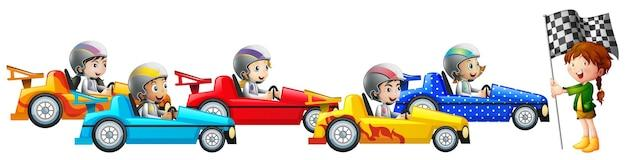
\includegraphics[width=4.15174in,height=1.06137in]{media/image1.jpg}

VOCÊ PERCEBEU COMO USAMOS OS NÚMEROS DE DIVERSAS FORMAS? ELES FORAM
ÚTEIS PARA NOS AJUDAR A CONTAR OS CARROS E A QUANTIDADE DE PARTICIPANTES
DA CORRIDA. ELES TAMBÉM NOS AJUDARAM A DEFINIR A CLASSIFICAÇÃO DOS
CORREDORES, E ATÉ NOS INDICARAM O VENCEDOR, OU SEJA, O PRIMEIRO A CRUZAR
A LINHA DE CHEGADA. ALÉM DISSO, OS NÚMEROS NÃO SERVEM SOMENTE PARA
CONTARMOS, MAS TAMBÉM PARA IDENTIFICARMOS ALGO. OS
AMIGOS CORREDORES DERAM NÚMEROS DE IDENTIFICAÇÃO A SEUS CARROS.
NOSSAS CASAS TAMBÉM TÊM NÚMEROS. ESSE É MAIS UM EXEMPLO DE
NÚMEROS IDENTIFICANDO, EM VEZ DE CONTAR.

\subsection{ATIVIDADES}\label{atividades}

\subsubsection{1. CIRCULE A FIGURA QUE CONTÉM UM NÚMERO USADO COMO
CÓDIGO DE
IDENTIFICAÇÃO.}\label{circule-a-figura-que-contuxe9m-um-nuxfamero-usado-como-cuxf3digo-de-identificauxe7uxe3o.}

\textless{}https://stock.adobe.com/br/images/id/363300782?get\_facets=1\&order=relevance\&safe\_search=1\&k=r\%C3\%A9gua\&clickref=1100lwwNzM24\&mv=affiliate\&mv2=Freepik\&as\_camptype=\&as\_channel=affiliate\&as\_source=partnerize\&as\_campaign=Freepik\&as\_content=api\&as\_audience=srp\&sdid=6WTV6YJ5;
https://stock.adobe.com/br/search?load\_type=search\&is\_recent\_search=\&search\_type=usertyped\&k=NUMERO+DE+CASA\&native\_visual\_search=\&similar\_content\_id=\&asset\_id=506848063;
https://stock.adobe.com/br/search?filters\%5Bcontent\_type\%3Aphoto\%5D=1\&filters\%5Bcontent\_type\%3Aillustration\%5D=1\&filters\%5Bcontent\_type\%3Azip\_vector\%5D=1\&filters\%5Bcontent\_type\%3Avideo\%5D=1\&filters\%5Bcontent\_type\%3Atemplate\%5D=1\&filters\%5Bcontent\_type\%3A3d\%5D=1\&filters\%5Bcontent\_type\%3Aimage\%5D=1\&order=relevance\&safe\_search=1\&limit=100\&search\_page=1\&k=1+KG\&search\_type=usertyped\&acp=\&aco=1+KG\&get\_facets=0\&asset\_id=418803262.
Inserir um diagrama com as 4 figuras, conforme modelo a seguir. É
importante que as imagens tenham um tamanho grande, para que os alunos
consigam enxergar os números.\textgreater{}

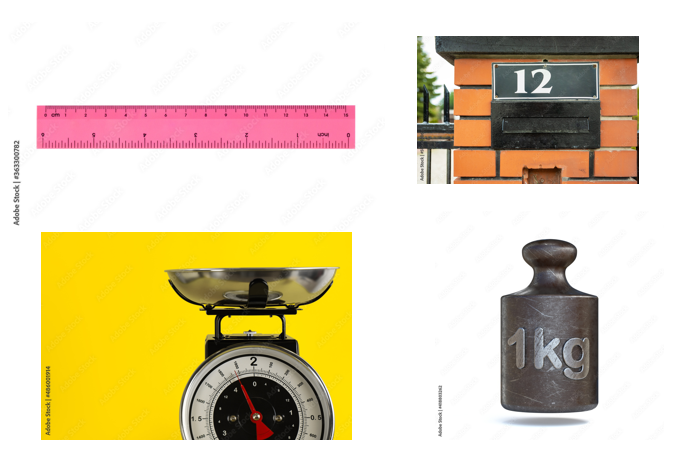
\includegraphics[width=3.98893in,height=2.65350in]{media/image2.png}

\coment{Somente na figura da caixa de correio, encontramos
um número identificador. Em todas as outras imagens, os números são usados para
quantificar medidas.}

\subsubsection{2. INDIQUE OS NÚMEROS DOS CARROS NA POSIÇÃO EM QUE
CRUZARAM A LINHA DE CHEGADA. CONSIDERE QUE NINGUÉM ULTRAPASSOU NINGUÉM.
}\label{indique-os-nuxfameros-dos-carros-na-posiuxe7uxe3o-em-que-cruzaram-a-linha-de-chegada.-ninguuxe9m-ultrapassou-ninguuxe9m}

\textless{}Inserir o diagrama a seguir conforme modelo. Licenciar a
figura:
https://br.freepik.com/vetores-gratis/no-jogo-de-corrida-de-velocidade-o-jogador-do-driver-do-monstro-da-competicao-usou-o-carro-de-alta-velocidade-para-vencer-no-jogo\_16304604.htm\#query=carros\%20com\%20n\%C3\%BAmeros\&position=11\&from\_view=search\&track=ais.\textgreater{}

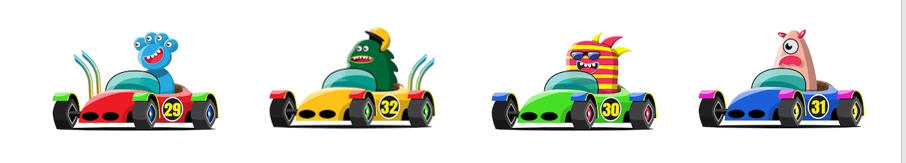
\includegraphics[width=5.90556in,height=1.06250in]{media/image3.png}

\textless{}Criar uma figura de um podium, com círculos acima das
posições, onde os alunos colocarão os números dos carros.\textgreater{}

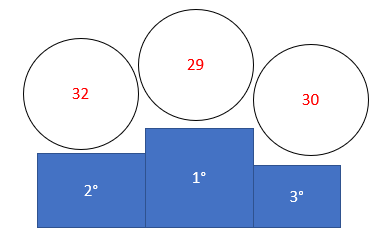
\includegraphics[width=3.92763in,height=2.54202in]{media/image4.png}

\coment{Oriente os alunos acerca das funções dos números de
identificação dos carros, destacando que eles não são os números que
indicarão a ordem de chegada deles. Oriente-os para que entendam que a
ordem se inicia da esquerda para a direita.}

\subsubsection{3. LIGUE OS NÚMEROS CORRETAMENTE.
}\label{ligue-os-nuxfameros-corretamente}

\begin{longtable}[]{@{}ll@{}}
\toprule
326 & CEM\tabularnewline
100 & CENTO E CINQUENTA E QUATRO\tabularnewline
154 & CENTO E QUARENTA\tabularnewline
451 & QUATROCENTOS E QUINZE\tabularnewline
514 & SEISCENTOS E VINTE E TRÊS\tabularnewline
140 & QUINHENTOS E CATORZE\tabularnewline
415 & TREZENTOS E VINTE E SEIS\tabularnewline
623 & QUATROCENTOS E CINQUENTA E UM\tabularnewline
\bottomrule
\end{longtable}


\subsubsection{4. ALBERTO TEM UMA COLEÇÃO DE CAMISAS DE FUTEBOL. JÚNIOR
TEM UMA COLEÇÃO DE BOLAS. QUAL DAS DUAS COLEÇÕES É A MAIOR?
}\label{alberto-tem-uma-coleuxe7uxe3o-de-camisas-de-futebol.-juxfanior-tem-uma-coleuxe7uxe3o-de-bolas.-qual-das-duas-coleuxe7uxf5es-uxe9-a-maior}

\textless{}Inserir figuras:
https://br.freepik.com/vetores-gratis/time-de-futebol-ou-jogadores-de-time-de-futebol-em-fundo-branco\_10600572.htm\#query=cole\%C3\%A7\%C3\%A3o\%20de\%20figurinhas\&position=11\&from\_view=search\&track=ais;
https://br.freepik.com/vetores-gratis/bolas-definir-ilustracao-vetorial\_4559016.htm\#query=cole\%C3\%A7\%C3\%A3o\%20de\%20bolas\&position=0\&from\_view=search\&track=ais.
Não precisa traduzir os textos em inglês, pois eles não são necessários
à resolução.\textgreater{}

\begin{quote}
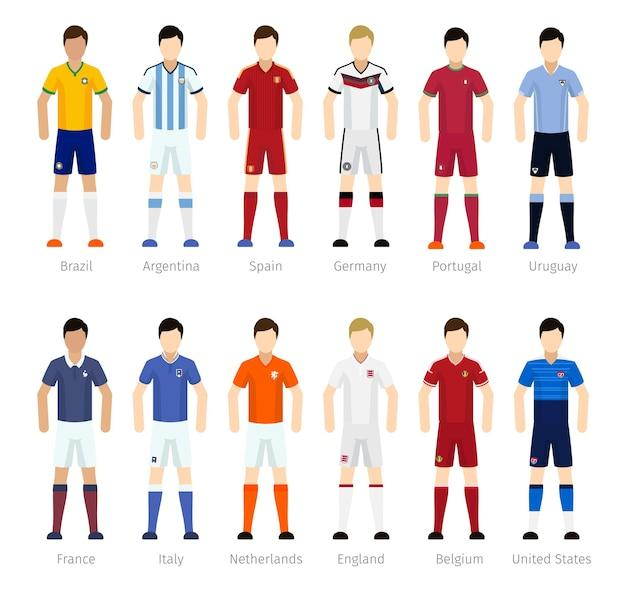
\includegraphics[width=2.90024in,height=2.77508in]{media/image5.jpg}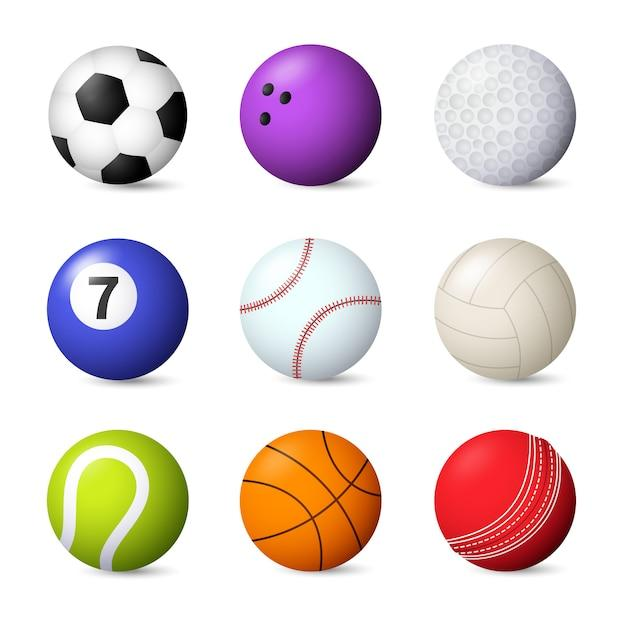
\includegraphics[width=2.59375in,height=2.59375in]{media/image6.jpg}
\end{quote}

\coment{O aluno deve contar as duas coleções e perceber que a coleção de camisas
de Alberto é maior, pois tem mais unidades do que a coleção de Júnior.}

\subsubsection{5. AINDA SOBRE A SITUAÇÃO APRESENTADA NA ATIVIDADE ANTERIOR, RESPONDA AO QUE SE PERGUNTA A SEGUIR.}\label{responda-mais-perguntas-sobre-a-atividade-anterior}

\begin{enumerate}
\def\labelenumi{\Alph{enumi})}
\item
  QUANTAS CAMISAS ALBERTO TEM? \textless{}1 linha\textgreater{}
\end{enumerate}

12 camisas.

\begin{enumerate}
\def\labelenumi{\Alph{enumi})}
\item
  QUANTAS BOLAS JÚNIOR TEM? \textless{}1 linha\textgreater{}
\end{enumerate}

9 bolas.

\begin{enumerate}
\def\labelenumi{\Alph{enumi})}
\item
  QUANTOS ITENS ALBERTO TEM EM SUA COLEÇÃO A MAIS QUE OS ITENS QUE JÚNIOR TEM EM SUA COLEÇÃO?
  \textless{}1 linha\textgreater{}
\end{enumerate}

3 itens.

\subsubsection{6. CIRCULE O CONJUNTO DE DADOS COM O MAIOR
RESULTADO.}\label{circule-o-conjunto-de-dados-com-o-maior-resultado}

\textless{} Inserir um quadro com as imagens conforme o modelo a seguir.
https://br.freepik.com/vetores-gratis/dados-isometricos-cubos-de-jogo-pretos-variantes-isolados-no-fundo-branco-coleta-de-todas-as-voltas-possiveis\_13090027.htm\#query=dice\&position=1\&from\_view=search\&track=sph.\textgreater{}

\begin{longtable}[]{@{}ll@{}}
\toprule
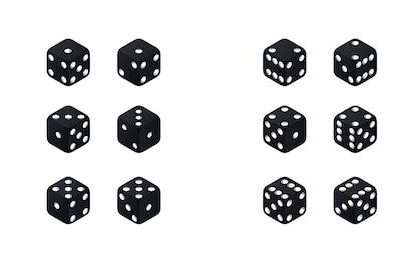
\includegraphics[width=1.85846in,height=2.68750in]{media/image7.jpg} &
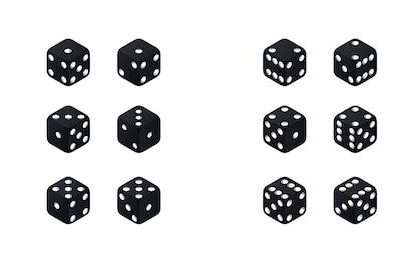
\includegraphics[width=1.57843in,height=2.68750in]{media/image7.jpg}\tabularnewline
\bottomrule
\end{longtable}

Oriente os alunos a olharem para o resultado da face
superior do dado, da mesma forma como eles fariam ao jogar um jogo
de tabuleiro. A imagem a ser circulada é a da direita,
pois a soma dos valores dos dados representados é maior do que a soma dos valores representados nos dados da imagem da esquerda.

\subsubsection{7. AINDA SOBRE A ATIVIDADE ANTERIOR, FAÇA O QUE SE PEDE A SEGUIR.}\label{aproveitando-a-atividade-anterior}

A. PINTE DE AZUL O QUADRADINHO QUE TEM O NÚMERO DA SOMA DOS DADOS DA
DIREITA.

B. PINTE DE VERDE O QUADRADINHO QUE TEM O NÚMERO DA SOMA DOS DADOS DA
ESQUERDA.

C. PINTE DE AMARELO A DIFERENÇA ENTRE AS DUAS SOMAS.

\begin{longtable}[]{@{}lllll@{}}
\toprule
12 & 24 & 30 & 40 & 10\tabularnewline
6 & 21 & 20 & 8 & 5\tabularnewline
7 & 18 & 4 & 22 & 13\tabularnewline
19 & 2 & 1 & 23 & 15\tabularnewline
25 & 11 & 9 & 17 & 32\tabularnewline
\bottomrule
\end{longtable}

O aluno deve pintar o número 18 de verde, o número 22 de azul e o número
4 de amarelo.

\subsubsection{8. ESCREVA OS SEGUINTES NÚMEROS EM ORDEM
CRESCENTE.}\label{escreva-os-seguintes-nuxfameros-em-ordem-crescente}
%PAULO: ANTES DE CADA SEQUÊNCIA DE NÚMEROS, TEM DE APARECER UMA LETRA, COMO ITENS DA ATIVIDADE.
516 -- 645 -- 215 -- 326 - 789

\begin{longtable}[]{@{}lllll@{}}
\toprule
215 & 326 & 516 & 645 & 789\tabularnewline
\bottomrule
\end{longtable}

132 -- 165 -- 112 -- 115 -- 100

\begin{longtable}[]{@{}lllll@{}}
\toprule
100 & 112 & 115 & 132 & 165\tabularnewline
\bottomrule
\end{longtable}

325 -- 854 -- 127 -- 974 -- 546

\begin{longtable}[]{@{}lllll@{}}
\toprule
127 & 325 & 546 & 854 & 974\tabularnewline
\bottomrule
\end{longtable}

415 -- 418 -- 411 -- 410 -- 417

\begin{longtable}[]{@{}lllll@{}}
\toprule
410 & 411 & 415 & 417 & 418\tabularnewline
\bottomrule
\end{longtable}

798 -- 987 -- 879 -- 897 -- 978

\begin{longtable}[]{@{}lllll@{}}
\toprule
798 & 879 & 897 & 978 & 987\tabularnewline
\bottomrule
\end{longtable}

623 -- 236 -- 362 -- 326 -- 263

\begin{longtable}[]{@{}lllll@{}}
\toprule
236 & 263 & 326 & 362 & 623\tabularnewline
\bottomrule
\end{longtable}

\subsubsection{9. ESCREVA OS SEGUINTES NÚMEROS EM ORDEM
DECRESCENTE.}\label{escreva-os-seguintes-nuxfameros-em-ordem-decrescente}

564 -- 456 -- 546 -- 645 -- 465

\begin{longtable}[]{@{}lllll@{}}
\toprule
645 & 564 & 546 & 465 & 456\tabularnewline
\bottomrule
\end{longtable}

138 -- 831 -- 318 -- 183 -- 813

\begin{longtable}[]{@{}lllll@{}}
\toprule
831 & 813 & 318 & 183 & 138\tabularnewline
\bottomrule
\end{longtable}

715 -- 517 -- 751 -- 571 -- 175

\begin{longtable}[]{@{}lllll@{}}
\toprule
751 & 715 & 571 & 517 & 175\tabularnewline
\bottomrule
\end{longtable}

833 -- 383 -- 838 -- 338 -- 388

\begin{longtable}[]{@{}lllll@{}}
\toprule
838 & 833 & 388 & 383 & 338\tabularnewline
\bottomrule
\end{longtable}

717 -- 177 -171 -- 117 -- 771

\begin{longtable}[]{@{}lllll@{}}
\toprule
771 & 717 & 177 & 171 & 117\tabularnewline
\bottomrule
\end{longtable}

100 -- 200 -- 300 - 400 -- 500

\begin{longtable}[]{@{}lllll@{}}
\toprule
500 & 400 & 300 & 200 & 100\tabularnewline
\bottomrule
\end{longtable}

\subsubsection{10. JERÔNIMO MORA NA CASA 328 DA RUA SANTOS, EM SUA
CIDADE. LIGUE CORRETAMENTE OS ALGARISMOS DO NÚMERO DA CASA ÀS ORDENS
CORRESPONDENTES.}\label{jeruxf4nimo-mora-na-casa-328-da-rua-santos-em-sua-cidade.-ligue-corretamente-os-algarismos-do-nuxfamero-da-casa-uxe0s-ordens-correspondentes}

\begin{longtable}[]{@{}ll@{}}
\toprule
3 & dezenas\tabularnewline
2 & centenas\tabularnewline
8 & unidades\tabularnewline
\bottomrule
\end{longtable}

\subsubsection{11. PINTE OS QUADRADOS COM A COR DA ORDEM CORRESPONDENTE.
}\label{pinte-os-quadrados-com-a-cor-da-ordem-correspondente}

\textless{}Criar um afigura conforme o modelo a seguir.\textgreater{}

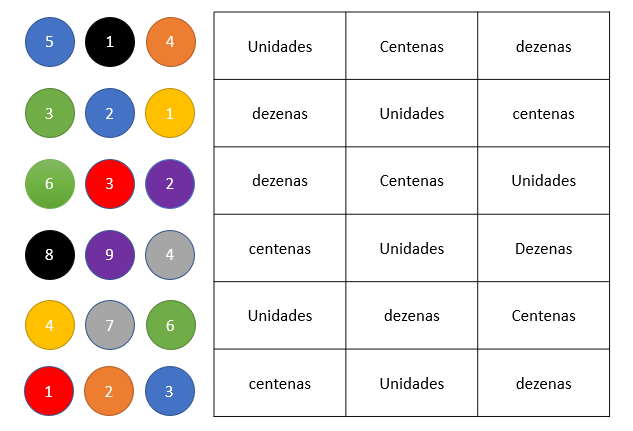
\includegraphics[width=5.90556in,height=4.02083in]{media/image8.png}

\begin{longtable}[]{@{}lll@{}}
\toprule
laranja & azul & Preto\tabularnewline
azul & amarelo & Verde\tabularnewline
vermelho & verde & Roxo\tabularnewline
preto & cinza & Roxo\tabularnewline
verde & cinza & Amarelo\tabularnewline
vermelho & azul & Laranja\tabularnewline
\bottomrule
\end{longtable}

\subsubsection{12. OS TRÊS COMPETIDORES REPRESENTADOS ESTÃO NO PÓDIO. ELES TÊM OS NOMES ESCRITOS NA CAMISETA. DESCUBRA QUAL É A PONTUAÇÃO DE CADA UM DELES E ESCREVA SEUS NOMES NA TABELA.}\label{section}

\textless{}Inserir a figura de referência:
https://br.freepik.com/vetores-gratis/podio-esportes\_1040693.htm\#query=podium\%20com\%20competidores\&position=1\&from\_view=search\&track=ais.
Acrescente os nomes dos competidores, conforme o modelo a
seguir.\textgreater{}

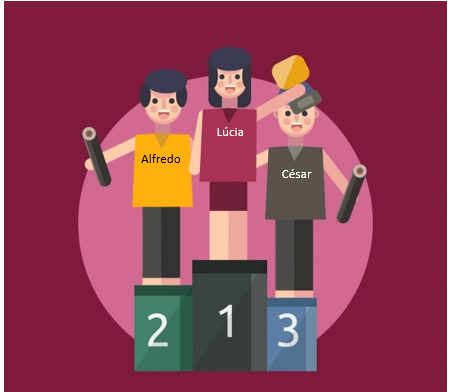
\includegraphics[width=3.84950in,height=3.34590in]{media/image9.png}

\begin{longtable}[]{@{}ll@{}}
\toprule
\textbf{PONTOS} & \textbf{NOMES}\tabularnewline
1~000 pontos & César\tabularnewline
1~005 pontos & Lúcia\tabularnewline
1~0004 pontos & Alfredo\tabularnewline
\bottomrule
\end{longtable}

É importante que os alunos compreendam que o primeiro
colocado deve ter feito a maior quantidade de pontos, e assim por
diante.

\subsubsection{13. A RETA NUMERADA A SEGUIR REPRESENTA UMA RUA QUALQUER DE UM BAIRRO. LIGUE AS CASAS ÀS SUAS RESPECTIVAS POSIÇÕES CONFORME O NÚMERO.}\label{section-1}

\textless{}Criar uma reta numérica conforme o modelo a seguir. Depois
colocar a figura de referência:
https://br.freepik.com/vetores-gratis/pacote-de-belas-fachadas-de-casas-desenhadas-a-mao\_1198631.htm\#page=2\&query=casas\%20coloridas\&position=11\&from\_view=search\&track=ais
com os respectivos números conforme o modelo.

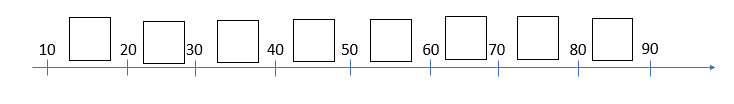
\includegraphics[width=5.90556in,height=0.83681in]{media/image10.png}

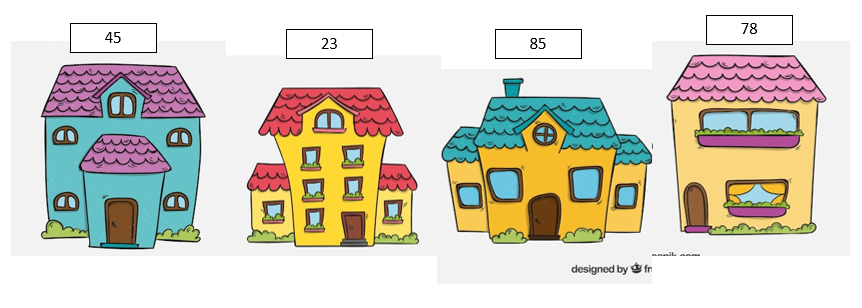
\includegraphics[width=5.90556in,height=2.10972in]{media/image11.png}

\subsubsection{14. ESCREVA OS NÚMEROS A SEGUIR COM ALGARISMOS.}\label{section-2}

\begin{longtable}[]{@{}ll@{}}
\toprule
Seiscentos e dezenove & 619\tabularnewline
oitocentos e trinta e sete & 837\tabularnewline
novecentos e quarenta e um & 941\tabularnewline
cento e dois & 102\tabularnewline
cento e trinta e oito & 138\tabularnewline
duzentos e vinte e cinco & 225\tabularnewline
trezentos e oitenta e quatro & 384\tabularnewline
quatrocentos e quinze & 415\tabularnewline
quinhentos e setenta e sete & 577\tabularnewline
setecentos e dezesseis & 716\tabularnewline
cento e cinquenta e três & 153\tabularnewline
\bottomrule
\end{longtable}

\subsubsection{}\label{section-3}

\subsection{TREINO}\label{treino}

\subsubsection{1. Na carteirinha da escola de Júlia, aparece sua foto, seu nome e o número do
registro de matrícula. No caso de Júlia, esse número é o 363. Esse número indica}\label{section-4}

\begin{enumerate}
\def\labelenumi{\Alph{enumi})}
\item
  quantidade.
\item
  ordem.
\item
  medida.
\item
  identificação.
\end{enumerate}

SAEB: Reconhecer o que os números naturais indicam em diferentes
situações: quantidade, ordem, medida ou código de identificação.
BNCC: EF01MA01 -- Utilizar números naturais como indicador de quantidade
ou de ordem em diferentes situações cotidianas e reconhecer situações em
que os números não indicam contagem nem ordem, mas sim código de
identificação.

\begin{enumerate}
\def\labelenumi{\alph{enumi})}
\item
  Incorreta. O número apresentado não representa quantidade ou contagem.
\item
  Incorreta. O número apresentado não apresenta necessariamente a ordem
  de matriculas feitas na escola.
\item
  Incorreta. O número não representa nenhuma unidade como metro ou
  grama.
\item
  Correta. Esse número é um código de identificação da aluna Júlia nos
  registros da escola.
\end{enumerate}

\subsubsection{2. Na imagem, mostram-se quatro coleções de amigos que gostam de colecionar
bolinhas de gude.}\label{section-5}

\textless{}Criar a figura conforme modelo a seguir.\textgreater{}

\begin{quote}
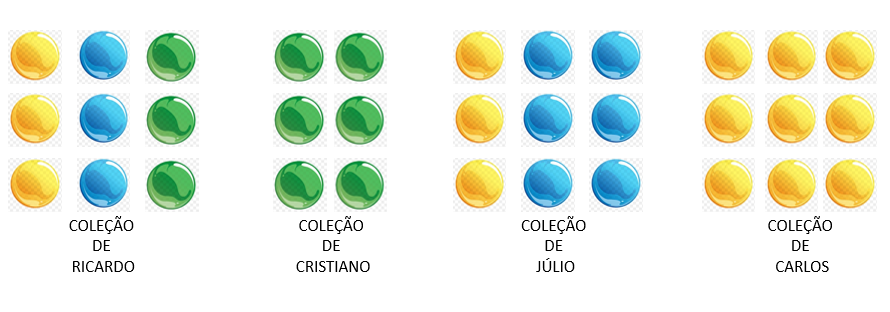
\includegraphics[width=5.90556in,height=2.07014in]{media/image12.png}
\end{quote}

Qual coleção tem a maior quantidade de bolas de uma única cor?

\begin{enumerate}
\def\labelenumi{\Alph{enumi})}
\item
  Carlos.
\item
  Cristiano.
\item
  Júlio.
\item
  Ricardo.
\end{enumerate}

SAEB: Comparar ou ordenar quantidade de objetos (até 2 ordens).

BNCC: EF01MA05 -- Comparar números naturais de até duas ordens em
situações cotidianas, com e sem suporte da reta numérica.

\begin{enumerate}
\def\labelenumi{\alph{enumi})}
\item
  Correta. Carlos tem a mesma quantidade de bolinhas que alguns amigos,
  porém todas são amarelas.
\item
  Incorreta. Cristiano só tem bolinhas verdes, porém tem menos do
  que Carlos.
\item
  Incorreta. Júlio tem bastante bolinhas azuis, porém em menor quantidade
  do que as amarelas de Carlos.
\item
  Incorreta. Ricardo tem poucas bolinhas de cada cor, apesar de ter o mesmo
  número total de Carlos.
\end{enumerate}

\subsubsection{3. ENTRE 0 E 100, QUANTOS NÚMEROS TERMINAM COM O NÚMERO ZERO NA ORDEM DAS UNIDADES?}\label{section-6}

\begin{enumerate}
\def\labelenumi{\Alph{enumi})}
\item
  1.
\item
  9.
\item
  10.
\item
  11.
\end{enumerate}

SAEB: Identificar a ordem ocupada por um algarismo OU seu valor
posicional (ou valor relativo) em um número natural de até 3 ordens.

BNCC: EF01MA03 -- Estimar e comparar quantidades de objetos de dois
conjuntos (em torno de 20 elementos), por estimativa e/ou por
correspondência (um a um, dois a dois) para indicar ``tem mais'', ``tem
menos'' ou ``tem a mesma quantidade''.

\begin{enumerate}
\def\labelenumi{\alph{enumi})}
\item
  Incorreta. O aluno pode ter considerado somente o zero, entendendo que
  não haveria outras ordens preenchidas.
\item
  Incorreta. O aluno pode ter se esquecido de considerar o zero e o cem.
\item
  Incorreta. O aluno pode ter se esquecido de considerar ou o zero ou
  o cem.
\item
  Correta. O aluno contou estes números: 0, 10, 20, 30, 40, 50, 60, 70, 80,
  90 e 100.
\end{enumerate}

\section{\texorpdfstring{\\
}{ }}\label{section-7}

\section{2. JUNTAR OU TIRAR?}\label{muxf3dulo-2-juntar-ou-tirar}

Neste módulo, vamos desenvolver a habilidade de desenvolvimento de
cálculos, tanto no sentido de escolher a melhor estratégia, quanto no
sentido de resolver o problema. Faremos essa abordagem de forma
abstrata, mas também de forma contextualizada, com o fim de desenvolver
nos alunos a motivação para resolverem problemas reais.
%PAULO: aplicar os estilos corretos nestes itens.
HABILIDADES DO SAEB:

- Calcular o resultado de adições e subtrações, envolvendo número
naturais de até 3 ordens.

- Compor ou decompor números naturais de até 3 ordens por meio de
diferentes adições.

- Resolver problemas de adição ou de subtração, envolvendo números
naturais de até 3 ordens, com os significados de juntar, acrescentar,
separar ou retirar.

HABILIDADES DA BNCC:
EF01MA07, EF01MA08.

\subsection{CONTEÚDO}\label{conteuxfado-1}

Márcia ganhou do pai duas notas de dez reais e decidiu que
queria comprar um brinquedo que custava quinze reais. márcia percebeu
que tinha um problema: para saber se ela teria condições de comprar
aquele brinquedo, ela teria de descobrir quanto dinheiro tinha, mas seu pai
resolveu ajudar. ele pegou a quantidade de palitos equivalente ao valor das
notas. observe:

\textless{}Criar uma ilustração com duas carreiras de 10 palitos
alinhadas a uma cédula de 10 reais, conforme o modelo a seguir.
https://www.istockphoto.com/br/foto/dez-real-brasileiro-gm181402095-26926813?utm\_campaign=srp\_photos\_inline\&utm\_content=https\%3A\%2F\%2Fwww.pexels.com\%2Fprocurar\%2F10\%2520reais\%2F\&utm\_medium=affiliate\&utm\_source=pexels\&utm\_term=10+reais

https://br.freepik.com/fotos-premium/uma-partida-com-cabeca-verde-em-um-fundo-branco\_31512045.htm\#page=3\&query=palito\%20de\%20f\%C3\%B3sforo\&position=18\&from\_view=search\&track=ais\textgreater{}

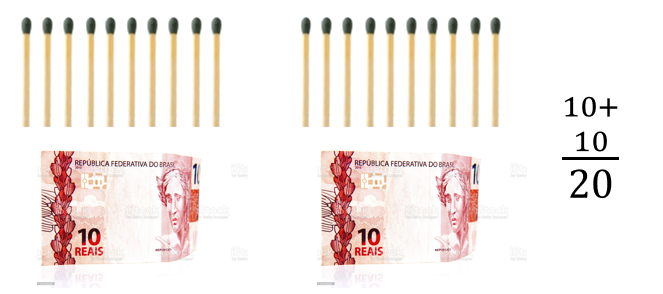
\includegraphics[width=3.31224in,height=1.46877in]{media/image13.png}

márcia contou os palitos e percebeu que tinha 20 reais. agora, ela
precisava saber se esses 20 reais seriam suficientes para comprar o
brinquedo. a própria márcia pegou mais quinze palitinhos e os alinhou da
seguinte forma:

\textless{}Criar uma figura com duas linhas de palito alinhados. Na
primeira linha 20 e na segunda linha 15. Colocar a operação ao lado,
conforme modelo a seguir.\textgreater{}

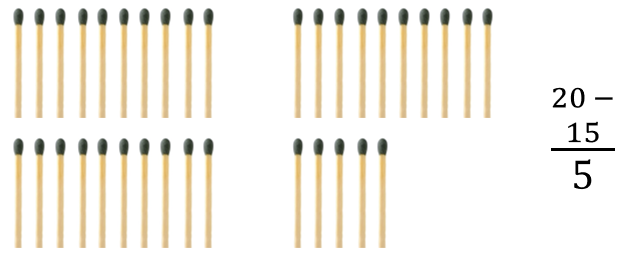
\includegraphics[width=3.31185in,height=1.38526in]{media/image14.png}

márcia ficou muito feliz ao perceber que poderia comprar seu brinquedo.
E ainda lhe sobrariam cinco reais para comprar um lanche.

\subsection{ATIVIDADES}\label{atividades-1}

\subsubsection{1}\label{section-8}

pinte o foguete com as cores corretas. descubra as cores resolvendo as
adições.

\textless{}Inserir um quadro conforme o modelo a seguir.
https://br.freepik.com/vetores-premium/foguete-de-desenho-bonito-de-cor-planilha-para
criancas\_22159996.htm\#page=6\&query=para\%20colorir\%20foguete\&position=7\&from\_view=search\&track=ais.\textgreater{}

\begin{longtable}[]{@{}lll@{}}
\toprule
59 & &
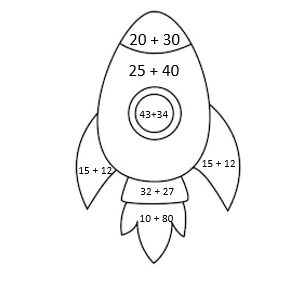
\includegraphics[width=3.09611in,height=2.97268in]{media/image15.png}\tabularnewline
65 & &\tabularnewline
77 & &\tabularnewline
90 & &\tabularnewline
50 & &\tabularnewline
27 & &\tabularnewline
\bottomrule
\end{longtable}

Oriente os alunos a resolverem as adições primeiro, antes
de começarem a pintar o foguete. No quadro à esquerda, temos as
resoluções das adições. Nele, o aluno deve pintar o pedaço do foguete com
a cor correspondente.

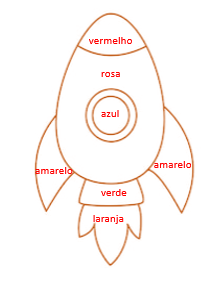
\includegraphics[width=1.43098in,height=1.89472in]{media/image16.png}

\subsubsection{2}\label{section-9}

efetue as adições a seguir.

\begin{longtable}[]{@{}llllllllll@{}}
\toprule
51 & + & 32 & + & 13 & + & 74 & + & 23 & +\tabularnewline
12 & & 21 & & 15 & & 20 & & 31 &\tabularnewline
63 & & 53 & & 28 & & 94 & & 54 &\tabularnewline
\bottomrule
\end{longtable}

\begin{longtable}[]{@{}llllllllll@{}}
\toprule
24 & + & 41 & + & 11 & + & 10 & + & 29 & +\tabularnewline
13 & & 36 & & 11 & & 60 & & 15 &\tabularnewline
37 & & 77 & & 22 & & 70 & & 44 &\tabularnewline
\bottomrule
\end{longtable}

Oriente os alunos a iniciarem as adições pela ordem das
unidades, seguindo pela ordem das dezenas e, finalmente, passando à das centenas,
para obter o resultado.

\subsubsection{3}\label{section-10}

efetue as subtrações a seguir.

\begin{longtable}[]{@{}llllllllll@{}}
\toprule
51 & - & 32 & - & 15 & - & 74 & - & 31 & -\tabularnewline
12 & & 21 & & 13 & & 20 & & 23 &\tabularnewline
39 & & 11 & & 2 & & 54 & & 8 &\tabularnewline
\bottomrule
\end{longtable}

\begin{longtable}[]{@{}llllllllll@{}}
\toprule
24 & - & 41 & - & 11 & - & 60 & - & 29 & -\tabularnewline
13 & & 36 & & 11 & & 10 & & 15 &\tabularnewline
11 & & 5 & & 0 & & 50 & & 14 &\tabularnewline
\bottomrule
\end{longtable}

Alguns termos desta atividade são iguais aos
termos da atividade anterior. É importante que você destaque isso com os
alunos, com o fim de que eles percebam que os resultados são diferentes,
em função da operação. É importante que percebam com clareza que os
resultados obtidos nas subtrações são sempre menores do que os
resultados obtidos nas adições quando os números envolvidos são os mesmos.

\subsubsection{4}\label{section-11}

PARA CONSEGUIR DAR O PRÓXIMO PASSO, O PATO PRECISA DESCOBRIR O PRÓXIMO VALOR. AJUDE-O.

\textless{}Criar um caminho conforme o modelo a seguir. As referências
dos patos são:
https://br.freepik.com/vetores-premium/desenho-de-pato-bonitinho-posando\_22341752.htm\#query=pato\&position=35\&from\_view=search\&track=sph

https://br.freepik.com/vetores-gratis/pato-fofo-em-branco\_7042481.htm\#query=pato\&position=0\&from\_view=search\&track=sph

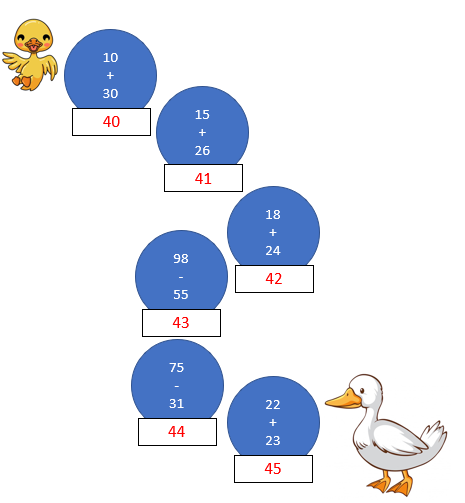
\includegraphics[width=4.84443in,height=5.24031in]{media/image17.png}

\subsubsection{5}\label{section-12}

PAULO tem uma coleção enorme de figurinhas: 20 figurinhas de
jogadores de futebol, 15 figurinhas de carros esportivos, 17 figurinhas
de jogos de \textit{videogame} e 26 figurinhas de seu personagem
preferido. na escola, PAULO perdeu 10 figurinhas, jogando tapão. com
quantas figurinhas ele ficou no total?
\textless{}4 linhas\textgreater{}

O aluno precisa
usar a adição e a subtração para obter a resposta. Oriente as crianças caso
estejam com dificuldade de encontrar a resposta correta, além de ler o
problema com eles, visto que ainda têm dificuldade de leitura e escrita.
Se necessário, distribua palitos para auxiliar os alunos na contagem.
Oriente-os a fazer uma adição por vez, assim como a fazer a subtração
somente no final.

\(15 + 17 + 26 = 58\) \(\rightarrow \ \ 58 - 10 = 48\).

\subsubsection{6}\label{section-13}

JOANA TEM MUITA VONTADE DE COMPARAR UMA BOLA NOVA, DEPOIS QUE PERDEU A QUE TINHA, E DESCOBRIU QUE, NA LOJA PERTO DE SUA CASA, UMA BEM LEGAL CUSTA 56 REAIS. A MENINA ABRIU SEU COFRINHO E CONTOU 25 REAIS, MAS JÁ CONTAVA COM A MESADA DE 15 REAIS QUE RECEBERIA NO FINAL DA SEMANA. QUANTO AINDA VAI FALTAR PARA JOANA COMPRAR A BOLA?
\textless{}4 linhas\textgreater{}


\subsubsection{7}\label{section-14}

demonstre várias formas de formarmos o numero 100 POR MEIO da adição de
duas parcelas.

\begin{longtable}[]{@{}llllllllll@{}}
\toprule
50 & + & & + & & + & & + & & +\tabularnewline
50 & & & & & & & & &\tabularnewline
100 & & 100 & & 100 & & 100 & & 100 &\tabularnewline
\bottomrule
\end{longtable}

\begin{longtable}[]{@{}llllllllll@{}}
\toprule
& + & & + & & + & & + & & +\tabularnewline
& & & & & & & & &\tabularnewline
100 & & 100 & & 100 & & 100 & & 100 &\tabularnewline
\bottomrule
\end{longtable}

Crie alguns
exemplos com os alunos e oriente-os a utilizarem números mais simples,
como 10, 20 etc. Aproveite para lembrar-lhes o conceito de parcelas,
pois, talvez, alguns não saibam ainda o que significa essa palavra.
A atividade pode ser aproveitada para ampliar o vocabulário dos alunos.

\subsubsection{8}\label{section-15}

demonstre várias formas de formarmos o numero 10 POR MEIO da subtração de
duas parcelas.

\begin{longtable}[]{@{}llllllllll@{}}
\toprule
100 & + & & + & & + & & + & & +\tabularnewline
90 & & & & & & & & &\tabularnewline
10 & & 10 & & 10 & & 10 & & 10 &\tabularnewline
\bottomrule
\end{longtable}

\begin{longtable}[]{@{}llllllllll@{}}
\toprule
& + & & + & & + & & + & & +\tabularnewline
& & & & & & & & &\tabularnewline
10 & & 10 & & 10 & & 10 & & 10 &\tabularnewline
\bottomrule
\end{longtable}


\subsubsection{9}\label{section-16}

resolva o enigma e descubra qual é o número. pinte-o no quadro.

- Sou maior que 5.

- sou menor que 50.

- uma das minhas parcelas pode ser 12.

- uma das minhas parcelas também pode ser 10.

- se uma das minhas parcelas for 20, a outra não pode ser maior do que
dois.

\begin{longtable}[]{@{}lll@{}}
\toprule
22 & 12 & 10\tabularnewline
32 & 50 & 5\tabularnewline
20 & 2 & 42\tabularnewline
\bottomrule
\end{longtable}

O número em questão é o 22.

\subsubsection{10}\label{section-17}

Pinte da mesma cor os números que, adicionados, em três parcelas, podem
formar os números que se pedem.

\begin{longtable}[]{@{}lllll@{}}
\toprule
2 & 10 & 5 & & 10\tabularnewline
25 & 3 & 22 & & 50\tabularnewline
28 & 50 & 15 & & 100\tabularnewline
\bottomrule
\end{longtable}

Explique aos alunos que só existe uma combinação possível
para cada número. Oriente também a pintarem as parcelas na cor
equivalente aos resultados esperados na coluna do lado direito. Peça
a eles que confiram antes de pintar. As combinações são:

\begin{longtable}[]{@{}lllll@{}}
\toprule
amarelo & verde & amarelo & & \(2 + 3 + 5 = 10\)\tabularnewline
verde & amarelo & azul & & \(25 + 10 + 15 = 50\)\tabularnewline
azul & azul & verde & & \(28 + 50 + 22 = 100\)\tabularnewline
\bottomrule
\end{longtable}

\subsubsection{11}\label{section-18}

patrick quer vender seu álbum de figurinhas por 56 reais. um amiguinho
quer COMPRÁ-LO, mas só tem 13 reais. além disso, só podera pagar o resto
em duas vezes, e a primeira parcela DEVErIA ser menor que a primeira.
ELABORE três formas de pagamento para o amigo de patrick.

\begin{longtable}[]{@{}lll@{}}
\toprule
& 56 -- 13 = & 43\tabularnewline
& &\tabularnewline
& menor & maior\tabularnewline
1° formato & 20 & 23\tabularnewline
& menor & maior\tabularnewline
2° formato & &\tabularnewline
& menor & maior\tabularnewline
3° formato & &\tabularnewline
\bottomrule
\end{longtable}

Oriente os
alunos a primeiro descobrirem quanto falta para o amigo de Patrick pagar
pelo álbum de figurinhas.

\subsubsection{12}\label{section-19}

assinale uma forma de agruparmos 45 reais utilizando as seguintes
cédulas.

\textless{}Criar uma figura conforme o modelo a seguir. Se necessário
desconfigure as notas de reais, contanto que as cédulas fictícias tenham
o mesmo valor. Coloque uma bola para que o aluno assinale.

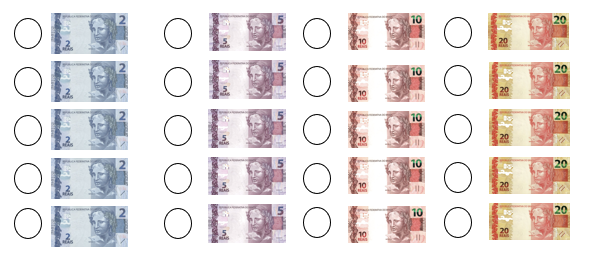
\includegraphics[width=5.90556in,height=2.71667in]{media/image18.png}

Há várias respostas possíveis. É
importante que o aluno consiga compreender a ideia de composição por
diferentes adições. Peça às crianças que criem outra forma além da
encontrada na atividade e registrem na lousa. Esta atividade é
importante para trabalhar educação financeira. Algumas das combinações
podem ser:

\(20 + 20 + 5,\ \ \ \ 10 + 10 + 10 + 10 + 5\), 2 + 2 + 2 + 2 + 2 + 10 + 20 + 5 etc.

\subsubsection{13}\label{section-20}

Numa partida de futebol, estavam jogando dois times: o time A e o time B. Foram marcados 10 gols, e o time a venceu a partida. Identidique os possíveis placares.

\textless{}Inserir uma figura conforme o modelo a seguir.
https://br.freepik.com/vetores-gratis/conjunto-de-simbolos-ou-emblemas-de-escudo-de-nove\_8998384.htm\#query=escudo\%20de\%20time\&position=5\&from\_view=search\&track=ais.\textgreater{}

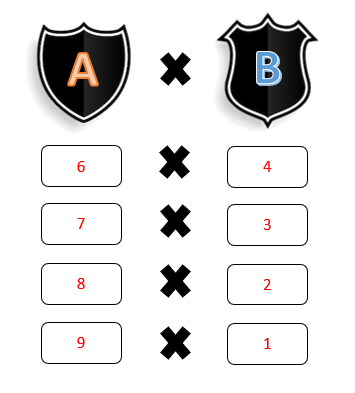
\includegraphics[width=2.78474in,height=3.08282in]{media/image19.png}

Oriente os alunos sobre o fato de haver exatamente quatro
resultados possíveis.

\subsubsection{14}\label{section-21}

a mãe de reinaldo vai chamar 50 pessoas para a festa de aniversário dele,
mas reinaldo tem 10 tios, 8 tias, 15 primos, 9 amigos e 4 vizinhos. Sobre essa situação, responda ao que se pergunta a seguir.

\begin{enumerate}
\def\labelenumi{\Alph{enumi})}
\item
  Convidando-se todas essas pessoas mencionadas, podem-se acrescentar convidados ou será necessário retirar pessoas da lista? \textless{}1 linha\textgreater{}
\end{enumerate}

O aluno precisa somar o número de pessoas: \(10 + 8 + 15 + 9 + 4 = 46\). Com isso, ele descobre que se podem acrescentar quatro pessoas ainda.

\begin{enumerate}
\def\labelenumi{\Alph{enumi})}
\item
  quantos convidados podem ser acrescentados ou quantas pessoas precisam ser retiradas? \textless{}1 linha\textgreater{}
\end{enumerate}

Subtraindo-se o número de pessoas da lista do número de convites para a festa, tem-se: \(50 - 46 = 4\ \). Podem ser convidadas ainda outras quatro pessoas.

\subsubsection{15}\label{section-22}

analise as caixas com as figuras geométricas. precisamos organizá-las para que cada caixa tenha a mesma quantidade de figuras. São 16 círculos, 16 quadrados e 16 triângulos; então cada caixa deve conter 4 quadrados, 4 triângulos e 4 círculos.

\textless{}Inserir uma figura com quatro caixas, identificadas por
letras, contendo círculos, quadrados e triângulos, espalhados de forma
aleatória, conforme o modelo a seguir.

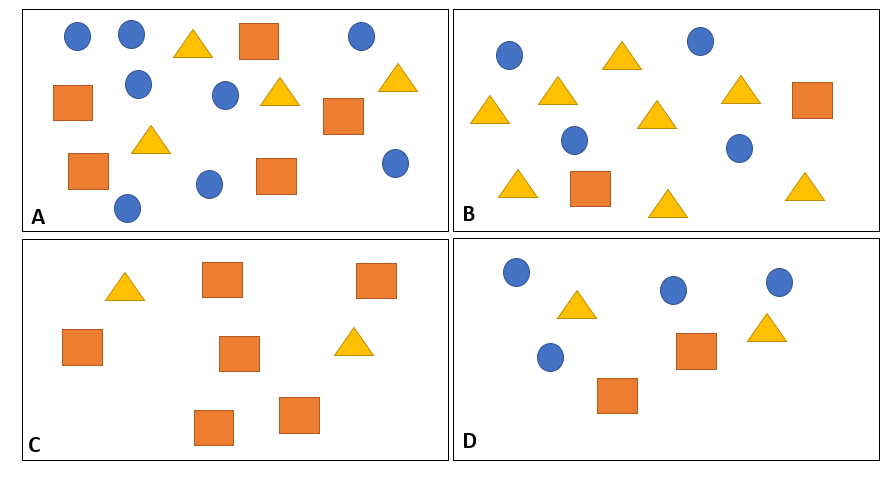
\includegraphics[width=5.90556in,height=3.22917in]{media/image20.png}

\begin{enumerate}
\def\labelenumi{\Alph{enumi})}
\item
  quantos círculos devem ser retirados da caixa \textbf{A}? \textless{}1
  linha\textgreater{}
\end{enumerate}

\begin{enumerate}
\def\labelenumi{\arabic{enumi}.}
\setcounter{enumi}{3}
\item
  círculos.
\end{enumerate}

\begin{enumerate}
\def\labelenumi{\Alph{enumi})}
\item
  quantos triângulos devem ser retirados da caixa \textbf{B}? \textless{}1
  linha\textgreater{}
\end{enumerate}

4 triângulos.

\begin{enumerate}
\def\labelenumi{\Alph{enumi})}
\item
  Quantos triângulos devem ser adicionados às caixas \textbf{C} e
  \textbf{D}? \textless{}1 linha\textgreater{}
\end{enumerate}

2 triângulos a cada uma.

\begin{enumerate}
\def\labelenumi{\Alph{enumi})}
\item
  quantos quadrados devem ser retirados da caixa \textbf{A}? \textless{}1
  linha\textgreater{}
\end{enumerate}

1 quadrado.

\begin{enumerate}
\def\labelenumi{\Alph{enumi})}
\item
  quantos quadrados devem ser retirados da caixa \textbf{C}? \textless{}1
  linha\textgreater{}
\end{enumerate}

2 quadrados.

\begin{enumerate}
\def\labelenumi{\Alph{enumi})}
\item
  quantos quadrados devem ser adicionados às caixas \textbf{B} e
  \textbf{D}? \textless{}1 linha\textgreater{}
\end{enumerate}

2 quadrados a cada uma.

\begin{enumerate}
\def\labelenumi{\Alph{enumi})}
\item
  Criando-se uma quinta caixa (\textbf{E}), com todas as figuras juntas, essa caixa \textbf{E} ficaria com quantas figuras?
\end{enumerate}

\(16 + 16 + 16 + 16 = 64\ \) figuras.

\subsection{TREINO}\label{treino-1}

\subsubsection{1}\label{section-23}

benício e bernardo são irmãos e resolveram juntar todas as
suas figurinhas: as 25 de benício e as 32 de bernardo. quantas figurinhas os
irmãos têm juntos?

\begin{enumerate}
\def\labelenumi{\Alph{enumi})}
\item
  7.
\item
  25.
\item
  32.
\item
  57.
\end{enumerate}

SAEB: Calcular o resultado de adições e subtrações, envolvendo
número naturais de até 3 ordens.
BNCC: EF01MA08 -- Resolver e elaborar problemas de adição e de subtração,
envolvendo números de até dois algarismos, com os significados de juntar, acrescentar, separar e retirar, com o suporte de imagens e/ou material manipulável, utilizando estratégias e formas de registro pessoais.

\begin{enumerate}
\def\labelenumi{\alph{enumi})}
\item
  Incorreta. O aluno pode ter subtraído ao invés de somar.
\item
  Incorreta. O aluno considerou somente as figurinhas de Benício.
\item
  Incorreta. O aluno considerou somente as figurinhas de Bernardo.
\item
  Correta. O aluno somou corretamente os dois valores: 25 + 32 = 57.
\end{enumerate}

\subsubsection{2}\label{section-24}

Em um colégio, o primeiro ano dividiu-se em dois times para jogarem basquete: o time Pequenos campeões e o time Basqueteiros. Ao todo, no jogo, os dois times fizeram 30 cestas, e os Pequenos campeões venceram os basqueteiros. Entre as opções a seguir, qual foi o placar final da partida?

\begin{enumerate}
\def\labelenumi{\Alph{enumi})}
\item
  Pequenos campeões 16 x Basqueteiros 15.
\item
  Pequenos campeões 16 x Basqueteiros 14.
\item
  Pequenos campeões 15 x Basqueteiros 14.
\item
  Pequenos campeões 15 x Basqueteiros 13.
\end{enumerate}

SAEB: Compor ou decompor números naturais de até 3 ordens por
meio de diferentes adições.
BNCC: EF01MA07 -- Compor e decompor número de até duas ordens, por meio
de diferentes adições, com o suporte de material manipulável,
contribuindo para a compreensão de características do sistema de
numeração decimal e o desenvolvimento de estratégias de cálculo.

\begin{enumerate}
\def\labelenumi{\alph{enumi})}
\item
  Incorreta. Adicionando-se 16 a 15, compõe-se o número 31, que é maior que o número de cestas da partida (30).
\item
  Correta. Adicionando-se 16 a 14, compõe-se a exata quantidade de cestas do
  jogo, ou seja, 30.
\item
  Incorreta. Adicionando-se 15 a 14, compõe-se o número 29, que é menor que o número de cestas da partida (30).
\item
  Incorreta. Adicionando-se 15 a 13, compõe-se o número 28, que é menor que o número de cestas da partida (30).
\end{enumerate}

\subsubsection{3}\label{section-25}

vinícius quer comprar um lanche, mas só tem 15 reais. pediu a sua mãe, e
ela lhe deu mais 12 reais. depois, pediu dinheiro à avó, e ela
lhe deu mais 10 reais. Então, vinícius percebeu que conseguiria comprar o lanche e um sorvete de 5 reais. qual é o preço do lanche?

\begin{enumerate}
\def\labelenumi{\Alph{enumi})}
\item
  15.
\item
  32.
\item
  37.
\item
  42.
\end{enumerate}

SAEB: Resolver problemas de adição ou de subtração, envolvendo
números naturais de até 3 ordens, com os significados de juntar,
acrescentar, separar ou retirar.
BNCC: EF01MA08 -- Resolver e elaborar problemas de adição e de subtração,
envolvendo números de até dois algarismos, com os significados de
juntar, acrescentar, separar e retirar, com o suporte de imagens e/ou
material manipulável, utilizando estratégias e formas de registro
pessoais.

\begin{enumerate}
\def\labelenumi{\alph{enumi})}
\item
  Incorreta. O aluno pode ter confundido o valor do lanche com o valor
  que Vinícius tinha.
\item
  Correta. O aluno acrescentou corretamente o valor do dinheiro que Vinícius tinha
  aos valores que ganhou e, então, retirou o valor do sorvete para
  descobrir o valor do lanche: \([(15 + 12 + 10) - 5] = 32\).
\item
  Incorreta. O aluno pode ter se esquecido de retirar o valor do sorvete.
\item
  Incorreta. O aluno acrescentou o valor do sorvete ao invés de retirar.
\end{enumerate}

\subsubsection{\texorpdfstring{\\
}{ }}\label{section-26}

\section{3. MAMÃE, ESTOU
CRESCENDO!}\label{muxf3dulo-3-mamuxe3e-estou-crescendo}

Neste módulo, vamos desenvolver as habilidades relativas
aos conceitos de massa, volume e comprimento. Desenvolver nos alunos a
ideia da necessidade de criarmos padrões de comparação para que medidas
sejam feitas com cada vez mais precisão.

Habilidades do SAEB

\begin{itemize}
\item
  Comparar comprimentos, capacidades ou massas ou ordenar imagens de
  objetos com base na comparação visual de seus comprimentos,
  capacidades ou massas.
\item
  Estimar/inferir medida de comprimento, capacidade ou massa de objetos,
  utilizando unidades de medida convencionais ou não ou medir
  comprimento, capacidade ou massa de objetos.
\item
  Identificar a medida de comprimento, da capacidade ou da massa de
  objetos, dada a imagem de um instrumento de medida.
\item
  Reconhecer unidades de medida e/ou instrumentos utilizados para medir
  comprimento, tempo, massa ou capacidade.
\end{itemize}

Habilidade da BNCC
EF01MA15

\subsection{CONTEÚDO}\label{conteuxfado-2}

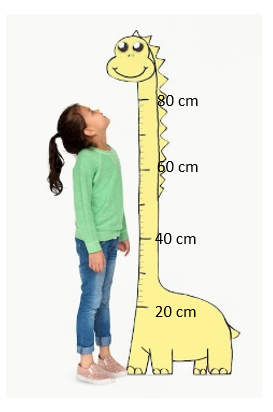
\includegraphics[width=1.67708in,height=2.53098in]{media/image21.png}

mariana é uma menina muito esperta, que cresce de forma saudável a cada
ano. sua mãe colou uma medidor na parede de seu quarto, e a cada ano
elas anotam a altura de mariana juntas.

\textless{}https://br.freepik.com/fotos-premium/escala-crescente-da-altura-alta-da-medida-da-crianca\_3375107.htm\#query=altura\%20de\%20crian\%C3\%A7a\&position=25\&from\_view=search\&track=ais.
Favor colocar as cotas de altura.\textgreater{}

Mariana está agora com 80 centímetros de \textbf{altura}, que, em geral, é a altura de uma mesa de escritório.
além disso, a mãe de mariana também comprou uma balança para medir seu
``peso'' -- que, na realidade, é sua massa. observe:

\textless{}https://br.freepik.com/vetores-premium/ilustracao-em-escala-industrial-em-fundo-transparente\_23844742.htm\#query=balan\%C3\%A7a\%20digital\&position=37\&from\_view=search\&track=ais.
Colocar o peso de Mariana em 18 kg.\textgreater{}

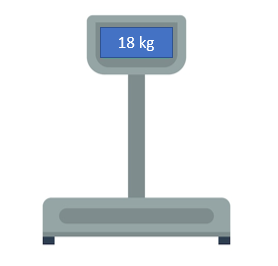
\includegraphics[width=2.13542in,height=2.04324in]{media/image22.png}

mariana está agora com 18 quilogramas de \textbf{massa}, ou seja, a mesma que uma poltrona pode ter. Se uma poltrona e mariana têm a mesma massa, por que a poltrona é
tão maior que mariana? cada corpo tem uma capacidade diferente de ocupar
espaço. essa capacidade é o que chamamos de \textbf{volume}.

para medirmos comprimentos, usamos a unidade metros, por exemplo. para medirmos massas, usamos a medida
quilograma, por exemplo. para medirmos o espaço ocupado, ou seja, o volume, usamos
a medida litro, por exemplo.

\subsection{ATIVIDADES }\label{atividades-2}

\subsubsection{1}\label{section-27}

cricule de azul o que compramos por quilograma (kg), de verde o que
compramos por litro (L) e de vermelho o que compramos por unidade.

\textless{}
https://br.freepik.com/vetores-premium/compra-de-mantimentos-frescos\_19552867.htm\#query=market\%20products\&position=9\&from\_view=search\&track=ais

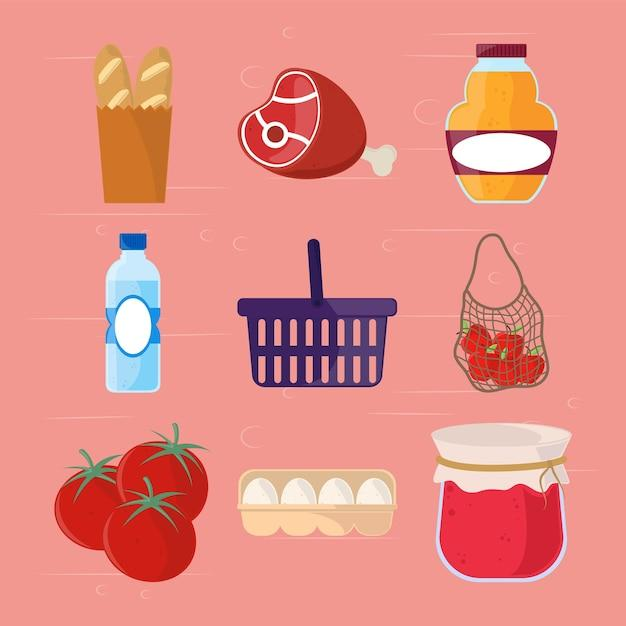
\includegraphics[width=3.53125in,height=3.53125in]{media/image23.jpg}

Oriente os alunos a se lembrarem das vezes em que foram ao
supermercado, por exemplo. Corrija a atividade com eles, mas permita que
eles tentem fazer sozinhos. Alguns dos itens são pedidos por unidades,
porém são pagos pela unidade de medidas, como é o caso dos pães. Se eles
colocarem na categoria do vendido por unidade, não considere erro, mas ressignifique, explicando
que, para o pagamento ser justo, é necessário que a cobrança seja feita, em alguns casos,
por quilograma ou litro. Assim, os alunos começam a perceber a real
importância das unidades de medida. Alguns alunos podem caracterizar a geleia como o vendido por litro. Se isso acontecer, explique
que somente líquidos são medidos assim e que massas pastosas são
medidas em quilogramas.

\subsubsection{2}\label{section-28}

Circule os itens que podem ser medidos em metros.

\textless{}Crie a figura conforme o modelo, utilizando as referências:
https://br.freepik.com/vetores-premium/mesa-de-madeira\_31804490.htm\#query=mesa\%20desenho\&position=5\&from\_view=search\&track=ais;
https://br.freepik.com/vetores-gratis/adesivo-de-pacote-de-saco-de-acucar-em-fundo-branco\_18055550.htm\#query=a\%C3\%A7ucar\%20desenho\&position=2\&from\_view=search\&track=ais
(traduzir -- açúcar);
https://br.freepik.com/vetores-gratis/fatia-de-queijo-saboroso\_3077481.htm\#query=queijo\%20desenho\&position=7\&from\_view=search\&track=ais;
https://br.freepik.com/vetores-gratis/beber\_23715247.htm\#query=refri\%20desenho\&position=9\&from\_view=search\&track=ais;
https://br.freepik.com/vetores-gratis/desenho-de-adesivo-com-rolo-de-corda-isolado\_18184169.htm\#query=cordadesenho\&position=0\&from\_view=search\&track=ais;
\href{https://br.freepik.com/vetores-premium/oleo-de-motor-de-substituicao-mecanico-de-automoveis-segurando-uma-lata-de-oleo-de-motor-isolado-no-fundo-branco-manutencao-do-servico-da-estacao-motor-e-mecanismos-de-lubrificacao-design-plano-de-ilustracao-vetorial_23005619.htm\#query=gasolina\%20gal\%C3\%A3odesenho\&position=6\&from_view=search\&track=ais}{\emph{https://br.freepik.com/vetores-premium/oleo-de-motor-de-substituicao-mecanico-de-automoveis-segurando-uma-lata-de-oleo-de-motor-isolado-no-fundo-branco-manutencao-do-servico-da-estacao-motor-e-mecanismos-de-lubrificacao-design-plano-de-ilustracao-vetorial\_23005619.htm\#query=gasolina\%20gal\%C3\%A3odesenho\&position=6\&from\_view=search\&track=ais}}.\textgreater{}

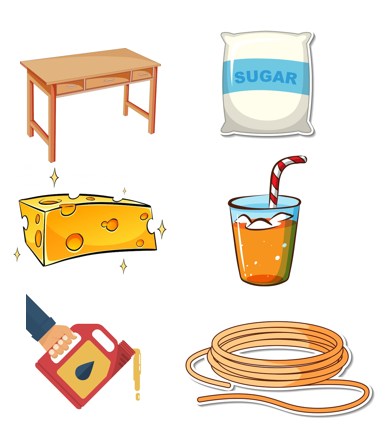
\includegraphics[width=4.02139in,height=4.59439in]{media/image24.png}

É importante que o aluno perceba que somente a mesa e a
corda podem ser medidas em metro.

\subsubsection{3}\label{section-29}

Ligue cada produto à unidade mais adequada para medi-lo.

\textless{}Inserir quadro conforme o modelo a seguir.\textgreater{}

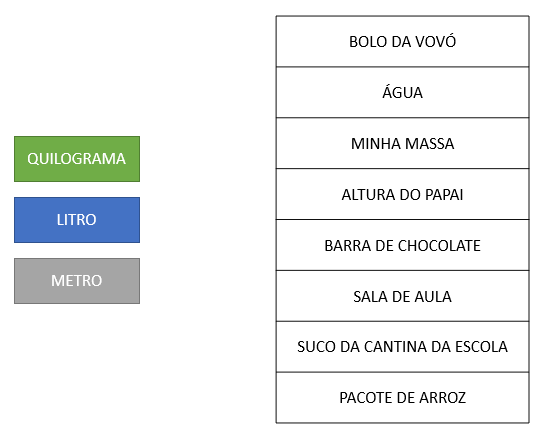
\includegraphics[width=4.86920in,height=3.96016in]{media/image25.png}

\subsubsection{4}\label{section-30}

Em cada quadro a seguir, desenhe ALGO QUE POSSA SER MEDIDO com o instrumento representado.

\textless{} insira os quadros e as figuras, conforme o modelo a seguir,
utilizando as referências:
https://br.freepik.com/vetores-premium/bonito-governante-engracado-acenando-o-personagem-de-mao\_23415941.htm\#page=3\&query=UMA\%20R\%C3\%89GUA\%20DESENHO\&position=39\&from\_view=search\&track=ais;
https://br.freepik.com/vetores-gratis/balanca-digital-em-fundo-branco\_16262850.htm\#query=BALAN\%C3\%87A\%20DESENHO\&position=3\&from\_view=search\&track=ais;
https://br.freepik.com/vetores-gratis/adesivo-de-copo-de-medicao-em-fundo-branco\_18180135.htm\#query=COPO\%20MEDIDORDESENHO\&position=2\&from\_view=search\&track=ais;
https://br.freepik.com/vetores-premium/fita-metrica-para-medir-a-distancia-em-centimetros-e-milimetros-rabiscar-a-coloracao-linear-dos-desenhos-animados\_30247681.htm\#query=TRENA\%20DESENHO\&position=45\&from\_view=search\&track=ais.\textgreater{}

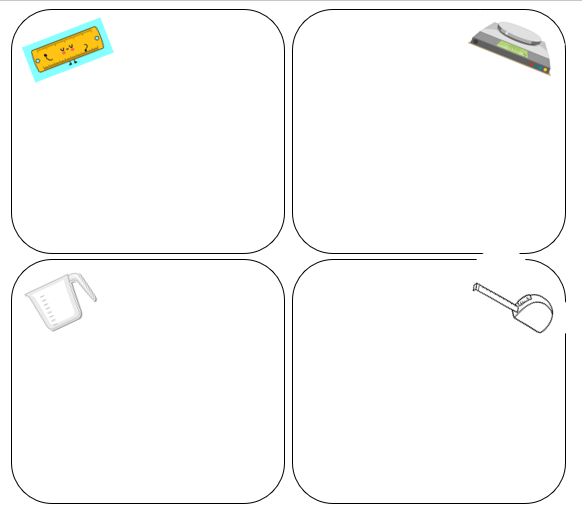
\includegraphics[width=6.43650in,height=5.62891in]{media/image26.png}

\subsubsection{5}\label{section-31}

Ligue cada pessoa à sua cama.

\textless{}Crie um quadro conforme o modelo a seguir, utilizando as
referências:
https://br.freepik.com/vetores-premium/homem-segurando-binoculos-pessoa-olhando-para-o-horizonte-futuro\_30928646.htm\#query=adulto\%20alto\%20DESENHO\&position=6\&from\_view=search\&track=ais;
https://br.freepik.com/vetores-premium/rapaz-dos-desenhos-animados-com-guitarra-criancas-tocando-instrumento-musical-em-casa-aula-ou-performance-artista-de-educacao-musical-ou-ferramentas-de-som-publicidade-vector-hobby-carreira-e-ilustracao-de-atividade-de-lazer\_26152103.htm\#query=adulto\%20baixo\%20DESENHO\&position=8\&from\_view=search\&track=ais;
https://br.freepik.com/vetores-gratis/personagem-de-desenho-animado-de-menino-bonito-em-fundo-branco\_28457881.htm\#query=menino\%20DESENHO\&position=5\&from\_view=search\&track=ais;
https://br.freepik.com/vetores-gratis/cama-com-travesseiro-e-lencol-azul\_2204447.htm\#query=cama\%20DESENHO\&position=1\&from\_view=search\&track=ais.\textgreater{}

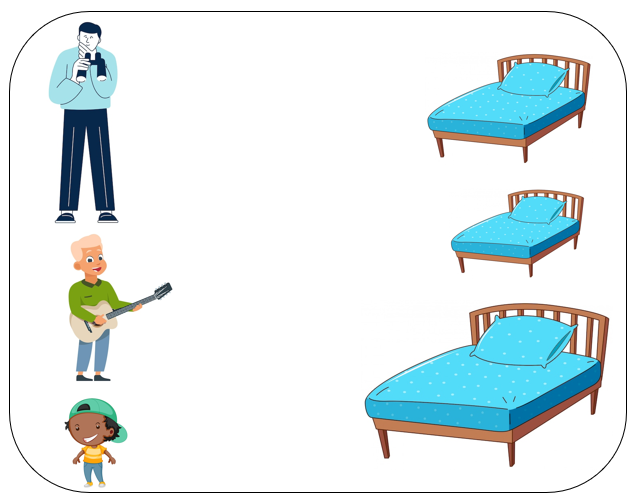
\includegraphics[width=6.28790in,height=4.93257in]{media/image27.png}

É importante que o aluno reconheça que as diferenças de
altura entre as pessoas se reflete na diferença de tamanho das camas.
É assim que o aluno conseguirá inferir a medida de comprimento.

\subsubsection{6}\label{section-32}

pinte como a jarra maior ficaria se for colocado nela todo o líquido das
jarras menores.

\protect\hypertarget{_heading=h.gjdgxs}{}{}\textless{}Inserir a figura
usando a referência:
https://br.freepik.com/vetores-gratis/adesivo-de-copo-de-medicao-em-fundo-branco\_18180135.htm\#query=COPO\%20MEDIDORDESENHO\&position=2\&from\_view=search\&track=ais.
Colocar as quantidades conforme o modelo a seguir.\textgreater{}

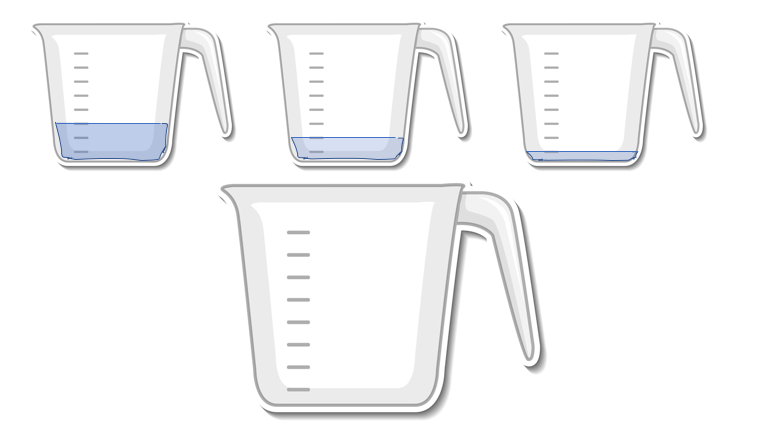
\includegraphics[width=5.90556in,height=3.37222in]{media/image28.png}

É importante desenvolver nos alunos uma capacidade de
medição empírica, já que não existe a unidade precisa na jarra.
Oriente os alunos a contarem a quantidade de riscos das jarras. Eles
devem pintar até a sexta marcação.

\subsubsection{7}\label{section-33}

ainda sobre a atividade anterior, se cada marcação da jarra maior medir meio litro,
quantos litros teriam sido colocados nela? \textless{}1
linha\textgreater{3 litros.}


\subsubsection{8}\label{section-34}

Qual é a capacidade total da jarra maior das atividades anteriores? Considere, mais uma vez, que cada marcação corresponde a meio litro.
\textless{}1 linha\textgreater{4 litros.}


\subsubsection{9}\label{section-35}

utilize uma régua e estime o comprimento de cada figura a seguir.

\textless{}Inserir os quadros com as figuras conforme os modelos a
seguir. Referências na figura.\textgreater{}

\begin{longtable}[]{@{}l@{}}
\toprule
\begin{minipage}[t]{0.97\columnwidth}\raggedright\strut
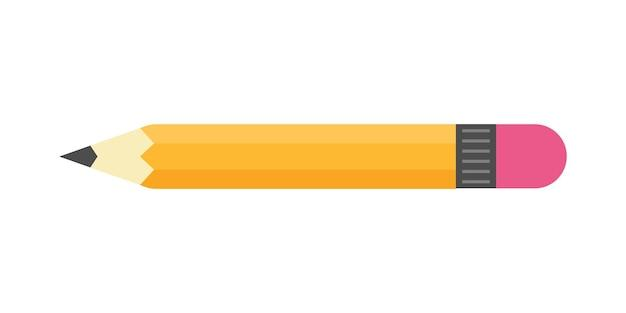
\includegraphics[width=5.91597in,height=0.90625in]{media/image29.jpg}

https://br.freepik.com/vetores-premium/icone-de-lapis-em-estilo-simples-ilustracao-vetorial-de-equipamentos-de-educacao-em-fundo-isolado-conceito-de-negocio-de-sinal-de-ferramenta-de-desenho\_30026502.htm\#query=lapis\&position=6\&from\_view=search\&track=sph\strut
\end{minipage}\tabularnewline
medida:\tabularnewline
\bottomrule
\end{longtable}

\begin{longtable}[]{@{}l@{}}
\toprule
\begin{minipage}[t]{0.97\columnwidth}\raggedright\strut
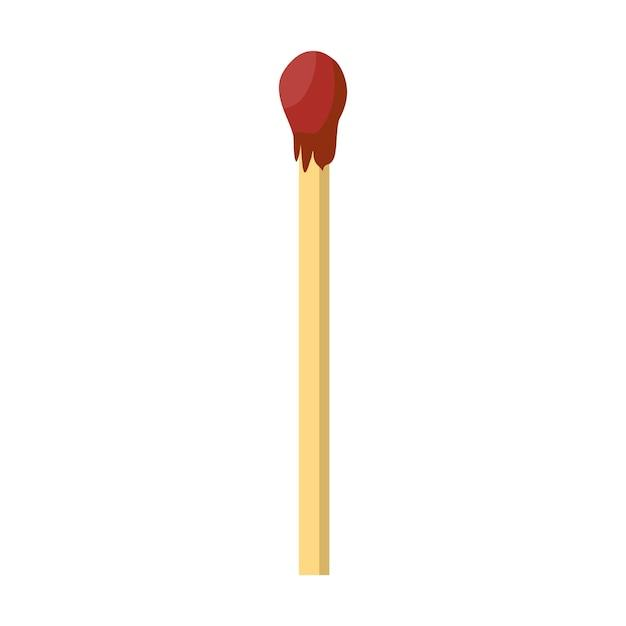
\includegraphics[width=0.69250in,height=4.62743in]{media/image30.jpg}

https://br.freepik.com/vetores-premium/objetos-vetoriais-isolados-de-desenho-animado-combinam-e-fogo\_29291308.htm\#query=palito\%20de\%20f\%C3\%B3sforo\%20desenho\&position=9\&from\_view=search\&track=ais\strut
\end{minipage}\tabularnewline
medida:\tabularnewline
\bottomrule
\end{longtable}

\begin{longtable}[]{@{}l@{}}
\toprule
\begin{minipage}[t]{0.97\columnwidth}\raggedright\strut
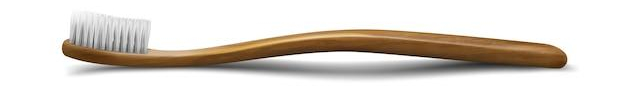
\includegraphics[width=5.90556in,height=0.75000in]{media/image31.jpg}

https://br.freepik.com/vetores-premium/objetos-vetoriais-isolados-de-desenho-animado-combinam-e-fogo\_29291308.htm\#query=palito\%20de\%20f\%C3\%B3sforo\%20desenho\&position=9\&from\_view=search\&track=ais\strut
\end{minipage}\tabularnewline
medida:\tabularnewline
\bottomrule
\end{longtable}

Oriente os alunos quanto ao fato de suas réguas medirem
comprimentos menores do que um metro. Explique que o centímetro
é uma subdivisão dessa unidade de medida. Este não é o momento de quantificar essa subdivisão.
Basta que entendam que se trata de outra unidade para medir
comprimentos.

\subsection{TREINO}\label{treino-2}

\subsubsection{1}\label{section-36}

Compare as alturas das crianças representadas a seguir.

\textless{}
https://br.freepik.com/vetores-gratis/quatro-criancas\_4906544.htm\#page=2\&query=crian\%C3\%A7as\%20com\%20diferentes\%20alturas\%20desenho\&position=13\&from\_view=search\&track=ais.\textgreater{}

A criança mais alta é

\begin{quote}
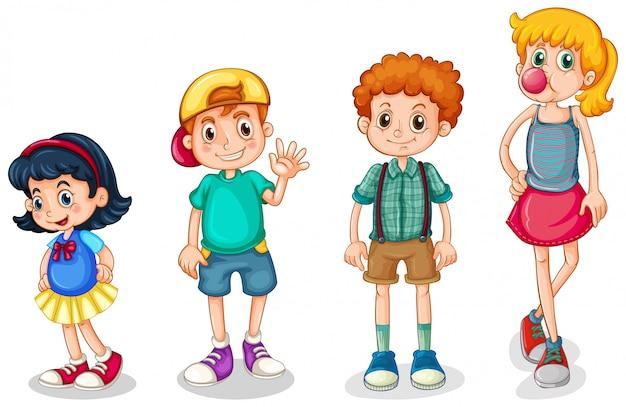
\includegraphics[width=4.23198in,height=2.75148in]{media/image32.jpg}
\end{quote}

A) a menina de saia amarela.

B) a menina mascando goma.

C) o menino de boné.

D) o menino de tênis azul.

SAEB: Comparar comprimentos, capacidades ou massas ou ordenar
imagens de objetos com base na comparação visual de seus comprimentos,
capacidades ou massas.
BNCC: EF01MA15 -- Comparar comprimentos, capacidades ou massas,
utilizando termos como mais alto, mais baixo, mais comprido, mais curto,
mais grosso, mais fino, mais largo, mais pesado, mais leve, cabe mais,
cabe menos, entre outros, para ordenar objetos de uso cotidiano.

a) Incorreta. A menina de saia amarela é a mais baixa.

b) Correta. A menina mascando goma tem a maior altura.

c) Incorreta. O menino de boné é o terceiro mais alto (ou o segundo mais
baixo).

d) Incorreta. O menino de tênis azul é o segundo mais alto.

\subsubsection{2. Observe esta imagem.}\label{section-37}

Paulo, inserir esta imagem:
https://br.freepik.com/vetores-gratis/mesa-de-centro-oval-preta-moderna-na-ilustracao-vetorial-realista-de-fundo-branco_23579954.htm#page=2&query=mesa&position=27&from_view=search&track=sph

Qual destes é o melhor instrumento de medida para se medir a distância do tampo da mesa até o chão?

\begin{quote}
A) uma balança

B) um copo de medição.

C) uma régua.

D) uma panela.

SAEB: Reconhecer unidades de medida e/ou instrumentos utilizados
para medir comprimento, tempo, massa ou capacidade.
BNCC: EF01MA15 -- Comparar comprimentos, capacidades ou massas,
utilizando termos como mais alto, mais baixo, mais comprido, mais curto,
mais grosso, mais fino, mais largo, mais pesado, mais leve, cabe mais,
cabe menos, entre outros, para ordenar objetos de uso cotidiano.

a) Incorreta. A balança é utilizada para medir massa em quilogramas.
\end{quote}

b) Incorreta. O copo de medição é utilizado para medir volume em litros ou mililitros.

c) Correta. A régua pode ser usada para medir a distância linear entre o tampo da mesa e o chão.

d) Incorreta. A panela só pode ser utilizada para medir volume.

\subsubsection{3. Veja a imagem.}\label{section-38}

\textless{}https://br.freepik.com/fotos-gratis/closeup-de-peso-escalas-conceito-de-excesso-de-peso-e-obesidade\_3219089.htm\#page=5\&query=regua\%20medindo\&position=49\&from\_view=search\&track=ais\textgreater{}

\begin{quote}
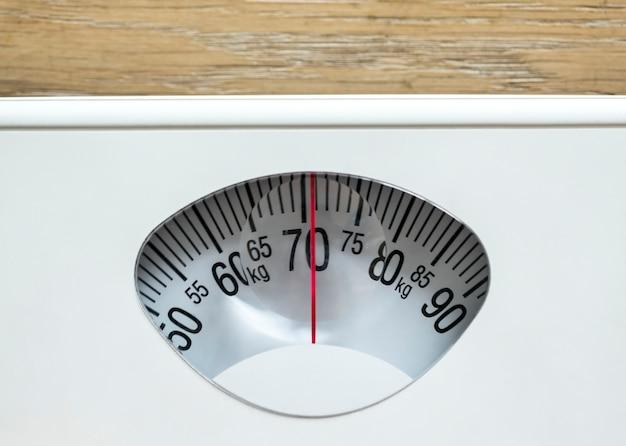
\includegraphics[width=3.03770in,height=1.48580in]{media/image33.jpg}
\end{quote}

Na imagem, mostra-se a medição da massa da mãe de juliana no visor da
balança. qual é a massa da mãe de juliana, medida em quilogramas?

A) 69.

B) 70.

C) 71.

D) 72.

SAEB: Identificar a medida de comprimento, da capacidade ou da
massa de objetos, dada a imagem de um instrumento de medida.
BNCC: EF01MA15 -- Comparar comprimentos, capacidades ou massas,
utilizando termos como mais alto, mais baixo, mais comprido, mais curto,
mais grosso, mais fino, mais largo, mais pesado, mais leve, cabe mais,
cabe menos, entre outros, para ordenar objetos de uso cotidiano.

a) Incorreta. O aluno pode ter invertido o sentido de leitura do visor.

b) Incorreta. O aluno entendeu que o ponteiro estava sobre o número 70.

c) Correta. O aluno percebeu que o ponteiro está deslocado uma unidade
além do 70.

d) Incorreta. O aluno deve ter pensado que cada marcação vale 2.

\section{4. EM QUE DIA DA SEMANA CAI MEU ANIVERSÁRIO?
}\label{muxf3dulo-4-em-que-dia-vai-cair-meu-aniversuxe1rio}

Neste módulo, vamos desenvolver nos alunos a habilidade de orientar-se no
tempo, sabendo identificar o tempo presente, assim como prever dias e
horários de eventos futuros.

Habilidades da BNCC
EF01MA16, EF01MA17, EF01MA18.

Habilidades do SAEB
- Identificar sequência de acontecimentos relativos a um dia.
- Identificar datas, dias da semana ou meses do ano em calendário ou
escrever uma data, apresentando o dia, o mês e o ano.
- Determinar a data de início, a data de término ou a duração de um
acontecimento entre duas datas.
- Determinar o horário de início, o horário de término ou a duração de
um acontecimento.

\subsection{CONTEÚDO}\label{conteuxfado-3}

É comum as pessoas ficarem ansiosas para chegar o dia do próprio aniversário!
não vemos a hora de ganhar presentes, comer bolo, assoprar a vela e
ficar com os amigos. Você sabe em que dia isso acontecerá? e em que dia
da semana? você sabe dizer a que horas vai começar ou terminar a 
festa de aniversário?

\textless{}https://br.freepik.com/vetores-premium/personagens-de-desenhos-animados-comemorando-a-festa-de-aniversario\_28760759.htm\#query=festa\%20de\%20aniversario\%20crian\%C3\%A7as\&position=10\&from\_view=search\&track=ais\textgreater{}

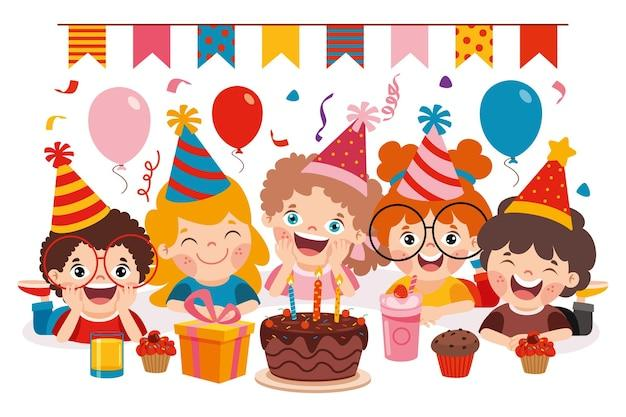
\includegraphics[width=4.02731in,height=2.68282in]{media/image34.jpg}

Vamos lembrar como é organizado nosso calendário.

o ano é dividido em 365 dias, e cada dia tem 24 horas. além disso, o ano
também é dividido em 12 meses, e os meses têm entre 28 e 31 dias. você lembra o nome dos meses e a quantidade
de dias de cada um? observe:

\begin{longtable}[]{@{}llllll@{}}
\toprule
Janeiro & Fevereiro & Março & abril & maio & junho\tabularnewline
31 dias & 28/29 dias & 31 dias & 30 dias & 31 dias & 30 dias\tabularnewline
Julho & agosto & setembro & outubro & novembro & dezembro\tabularnewline
31 dias & 31 dias & 30 dias & 31 dias & 30 dias & 31 dias\tabularnewline
\bottomrule
\end{longtable}

Os meses estão organizados em semanas, que são divididas em 7 dias. observe os nomes
desses dias:

\begin{longtable}[]{@{}lllllll@{}}
\toprule
domingo & segunda-feira & terça-feira & quarta-feira & quinta-feira & sexta-feira &
sábado\tabularnewline
\bottomrule
\end{longtable}

\subsection{ATIVIDADES}\label{atividades-3}

\subsubsection{1}\label{section-39}

vamos descobrir que dia é hoje? escreva o que se pede a seguir.

\begin{longtable}[]{@{}ll@{}}
\toprule
em que ano estamos? &\tabularnewline
em que mês estamos? &\tabularnewline
que dia do mês é hoje? &\tabularnewline
que dia da semana é hoje? &\tabularnewline
que horas são neste momento em que você está resolvendo esta atividade? & : :\tabularnewline
\bottomrule
\end{longtable}

O mais importante nesta atividade é fazer com que o aluno
consiga diferenciar cada classificação do tempo, como saber diferenciar dia
do mês e dia da semana, por exemplo. Oriente-os a preencherem o horário
com horas, minutos e segundos. Essa atividade pode e deve ser usada com
fins de avaliação diagnóstica.

\subsubsection{2}\label{section-40}

pinte os quadrados com a cor equivalente.

\begin{longtable}[]{@{}lllll@{}}
\toprule
Domingo & 30 & Março & 2022 & 13:15:00\tabularnewline
mês & ano & horário & dia do mês & dia da semana\tabularnewline
\bottomrule
\end{longtable}

A sequência de cores é: amarelo, vermelho, laranja, verde e azul.

\subsubsection{3}\label{section-41}

Circule no calendário o dia do seu aniversário e anote em que dia da semana ele está.

\textless{}
https://br.freepik.com/vetores-premium/calendario-de-cores-para-2023-com-um-coelho-de-personagem-fofo-a-semana-comeca-no-domingo-diversao-e-estilo-de-desenho-animado-de-design-brilhante\_34560382.htm\#query=calend\%C3\%A1rio\%20infantil\%202023\%20em\%20portugu\%C3\%AAs\&position=6\&from\_view=search\&track=ais.
Traduzir os nomes dos meses, além das iniciais dos dias da
semana.\textgreater{}

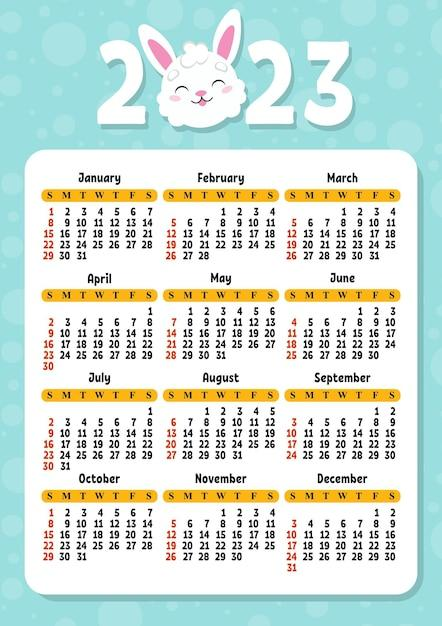
\includegraphics[width=4.71050in,height=6.67143in]{media/image35.jpg}


\subsubsection{4}\label{section-42}

analise as figuras e liste a ordem dos acontecimentos em um dia.

\textless{}Inserir as figuras na ordem do modelo a seguir. Utilizar as
referências:
https://br.freepik.com/vetores-premium/garoto-bonito-comendo-delicioso-arroz-frito\_35549113.htm\#query=crian\%C3\%A7a\%20almo\%C3\%A7ando\&position=48\&from\_view=search\&track=ais;
https://br.freepik.com/vetores-gratis/menino-dormir-cama\_4388324.htm\#query=crian\%C3\%A7a\%20acordando\&position=21\&from\_view=search\&track=ais;
https://br.freepik.com/vetores-gratis/menino-que-dorme-na-cama\_1021842.htm\#query=crian\%C3\%A7a\%20acordando\&position=23\&from\_view=search\&track=ais;
https://br.freepik.com/vetores-gratis/uma-garota-fazendo-o-exame\_2607446.htm\#query=crian\%C3\%A7a\%20estudasndo\&position=0\&from\_view=search\&track=ais
e
https://br.freepik.com/vetores-gratis/criancas-felizes-brincando-com-brinquedos\_11575551.htm\#query=crian\%C3\%A7a\%20brincando\&position=32\&from\_view=search\&track=ais
\textgreater{}

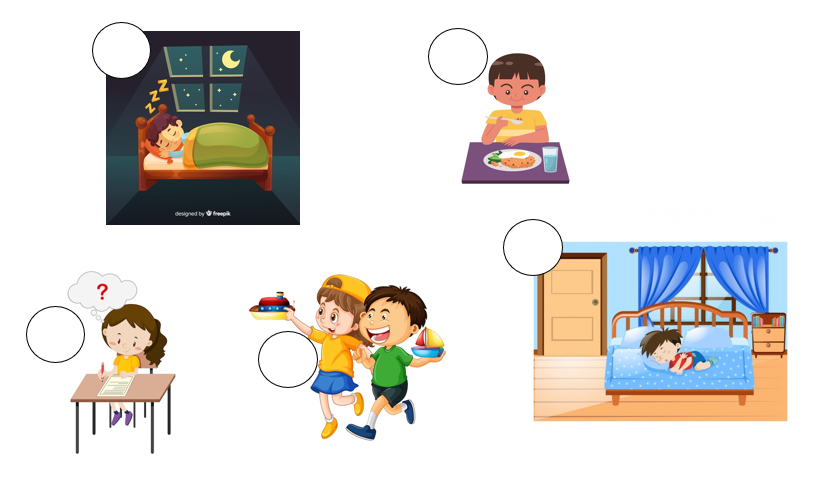
\includegraphics[width=5.90556in,height=3.46597in]{media/image36.png}

Espera-se que os alunos sigam a ordem dos acontecimentos
baseando-se nas próprias rotinas. Aproveite para frisar a importância de
se alimentar no horário certo, além de
ressaltar a importância de priorizar o momento dos estudos, ou seja,
estudar antes de brincar. Esta atividade pode ser utilizada também para
os alunos lembrarem a utilização dos números para ordenar.
Oriente-os a utilizarem os números de forma ordinal (1º, 2º, 3º etc.).

\subsubsection{5}\label{section-43}

Complete oS QUADRADOS EM BRANCO DO calendário a seguir.

\begin{longtable}[]{@{}l@{}}
\toprule
JANEIRO 2023\tabularnewline
Dom\tabularnewline
1\tabularnewline
8\tabularnewline
15\tabularnewline
22\tabularnewline
29\tabularnewline
\bottomrule
\end{longtable}

Os alunos devem preencher os quadrados faltantes dos
dias do mês, assim como dos dias da semana.

\subsubsection{6}\label{section-44}

baseando-se no calendário da atividade anterior, responda ao que se pergunta a seguir.

\begin{enumerate}
\def\labelenumi{\Alph{enumi})}
\item
  Em que dia da semana está o dia 18 de janeiro?
\end{enumerate}

\textless{}1linha\textgreater{}

Quarta-feira.

\begin{enumerate}
\def\labelenumi{\Alph{enumi})}
\item
  quantos sábados existem em janeiro de 2023?
\end{enumerate}

\textless{}1linha\textgreater{}

São quatro sábados.

\begin{enumerate}
\def\labelenumi{\Alph{enumi})}
\item
  em que dia da semana começa esse mês de janeiro?
\end{enumerate}

\textless{}1linha\textgreater{}

Domingo.

\begin{enumerate}
\def\labelenumi{\Alph{enumi})}
\item
  em que dia da semana termina esse mês de janeiro?
\end{enumerate}

\textless{}1linha\textgreater{}

Terça-feira.

\begin{enumerate}
\def\labelenumi{\Alph{enumi})}
\item
  quantos domingos existem nesse mês de janeiro?
\end{enumerate}

\textless{}1linha\textgreater{}

São cinco domingos.

Aproveite para demonstrar que, em alguns meses,
pode haver algum dia da semana se repetindo cinco vezes, ou seja, o fato de
haver quatro semanas em um mês não significa que haverá sempre quatro repetições
de cada dia da semana. Esta atividade é importante para desenvolver no
aluno a habilidade de ler o calendário com entendimento.

\subsubsection{7}\label{section-45}

Analise o bloco de notas de marcela. Quantos dias ela esperará
pela resposta de que precisa?

\textless{}Inserir a figura da referência:
https://br.freepik.com/vetores-premium/caderno-e-lapis-em-fundo-branco\_10079541.htm\#query=bloco\%20de\%20anota\%C3\%A7\%C3\%B5es\&position=10\&from\_view=search\&track=ais,
incluindo o texto conforme o modelo:\textgreater{}

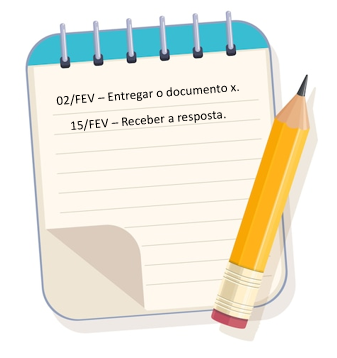
\includegraphics[width=3.51091in,height=3.72969in]{media/image37.png}

Entre os dias 2 e 15, passam-se 13 dias.

\subsubsection{8}\label{section-46}

Se o dia da semana em que marcela entregou o documento fosse
sexta-feira, em que dia da semana cairia o dia da resposta?

\textless{}1 linha\textgreater{}

Quinta-feira.

\subsubsection{9}\label{section-47}

Em uma escola, uma competição de futebol de salão durou sete dias.
Se a competição começou no dia 10 de outubro de 2021, um sábado, em que
data terminou o campeonato?

\begin{longtable}[]{@{}ll@{}}
\toprule
ano: & 2021\tabularnewline
mês: & Outubro\tabularnewline
dia do mês: & 16\tabularnewline
dia da semana: & Sexta-feira\tabularnewline
\bottomrule
\end{longtable}


\subsubsection{10}\label{section-48}

analise os relógios digitais da imagem. Depois, responda ao que se pergunta a seguir.

\textless{}Inserir a figura da referência:
https://br.freepik.com/vetores-premium/um-conjunto-de-relogios-digitais-numeros-eletronicos-ilustracao-vetorial\_32708528.htm\#query=rel\%C3\%B3gio\%20digital\&position=16\&from\_view=search\&track=ais,
inserindo as identificações dos relógios, conforme o modelo a
seguir.\textgreater{}

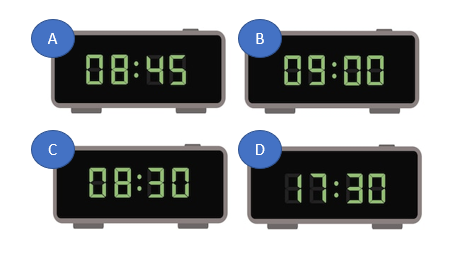
\includegraphics[width=4.34174in,height=2.58209in]{media/image38.png}

\begin{enumerate}
\def\labelenumi{\Alph{enumi})}
\item
  Qual é a diferença entre o horário do relógio \textbf{A} e o do relógio \textbf{B}?
\end{enumerate}

\textless{}1linha\textgreater{}

Uma hora e quarenta e cinco minutos. 01:45:00.

\begin{enumerate}
\def\labelenumi{\Alph{enumi})}
\item
  Qual é a diferença entre o horário do relógio \textbf{C} e o do relógio \textbf{A}?
\end{enumerate}

\textless{}1 linha\textgreater{}

Quinze minutos. 00:15:00.

\begin{enumerate}
\def\labelenumi{\Alph{enumi})}
\item
  Qual é a diferença entre o horário do relógio \textbf{B} e o do relógio \textbf{D}?
\end{enumerate}

\textless{}1 linha\textgreater{}

Oito horas e trinta minutos. 08:30:00.

\begin{enumerate}
\def\labelenumi{\Alph{enumi})}
\item
  Qual é a diferença entre o horário do relógio \textbf{C} e o do relógio \textbf{D}?
\end{enumerate}

\textless{}1 linha\textgreater{}

Nove horas. 09:00:00.

Oriente os alunos a darem respostas neste formato: hh:mm:ss.

\subsubsection{11}\label{section-49}

Para acordar, Mariano ajustou o alarme do celular para o horário mostrado a seguir.

\textless{}https://br.freepik.com/vetores-gratis/smartphone-de-tela-de-alarme\_2921841.htm\#query=relogio\%20celular\&position=48\&from\_view=search\&track=ais.\textgreater{}

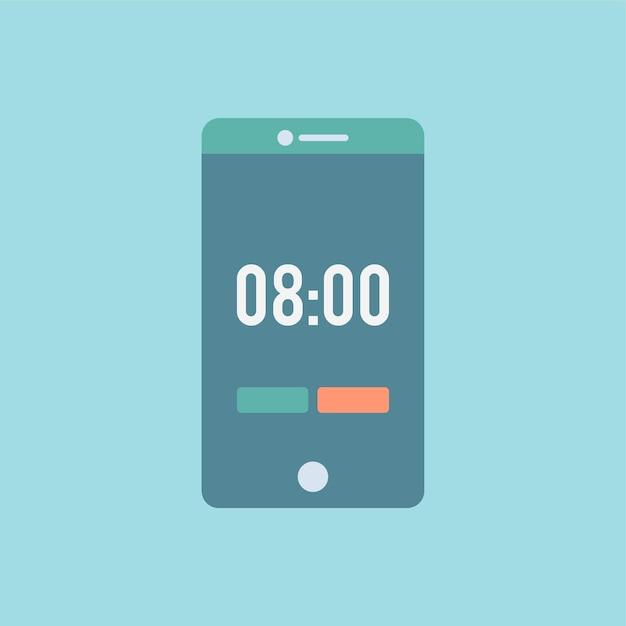
\includegraphics[width=1.70922in,height=2.53170in]{media/image39.jpg}

ele levantou-se, arrumou-se, tomou café da manhã e foi para o trabalho. Chegou ao trabalho 1 hora e 35 minutos depois de acordar. A que horas ele chegou ao trabalho?

\textless{}1 linha\textgreater{}

09:35:00.

\subsubsection{12}\label{section-50}

PEDRO ACORDOU ÀS 07:30 DA MANHÃ.

https://br.freepik.com/vetores-gratis/um-menino-dormindo-profundamente\_23807622.htm\#query=PEDRINHO\%20ACORDANDO\&position=5\&from\_view=search\&track=ais.\textgreater{};
https://br.freepik.com/vetores-gratis/menino-de-pijama-segurando-a-escova-de-dentes-e-pasta-de-dente\_27547013.htm\#query=ESCOVAR\%20OS\%20DENTES\&position=32\&from\_view=search\&track=ais
https://br.freepik.com/vetores-gratis/um-menino-feliz-comendo-na-mesa\_18973385.htm\#query=CAF\%C3\%81\%20DA\%20MANH\%C3\%83\%20MENINO\&position=12\&from\_view=search\&track=ais;
https://br.freepik.com/vetores-premium/um-menino-brincando-com-gato-fofo\_29183474.htm\#page=2\&query=BRINCANDO\%20COM\%20O\%20GATO\&position=6\&from\_view=search\&track=ais.
\textgreater{}

\begin{quote}
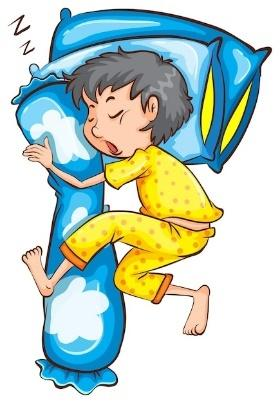
\includegraphics[width=1.27248in,height=1.83120in]{media/image40.jpg}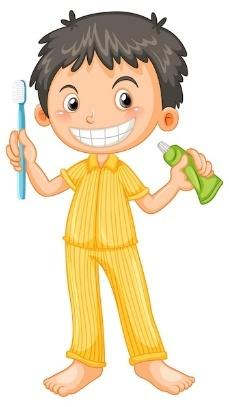
\includegraphics[width=1.04250in,height=1.85399in]{media/image41.jpg}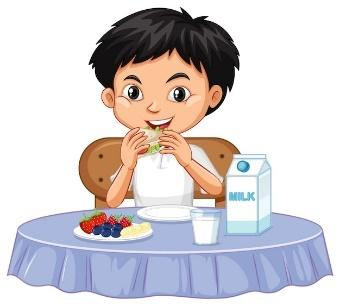
\includegraphics[width=1.54748in,height=1.39171in]{media/image42.jpg}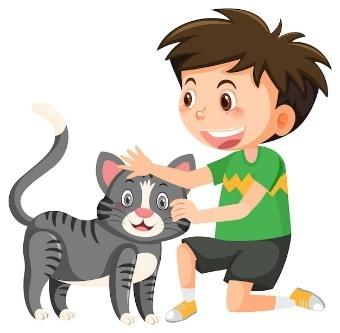
\includegraphics[width=1.54490in,height=1.51274in]{media/image43.jpg}

DEPOIS, DEMOROU 15 MINUTOS PARA IR AO BANHEIRO E ESCOVAR OS DENTES.
DEMOROU MAIS 20 MINUTOS PARA TOMAR O CAFÉ DA MANHÃ. ANTES DE SAIR,
AINDA FICOU 5 MINUTOS BRINCANDO COM O GATO. ENTÃO SAIU PARA A ESCOLA.

PINTE NO RELÓGIO A SEGUIR O HORÁRIO EM QUE PEDRO SAIU PARA IR À ESCOLA.
\end{quote}

\textless{}Inserir uma figura de um relógio, com os números em branco
para o aluno preencher, conforme o modelo a seguir:\textgreater{}


\includegraphics[width=5.90556in,height=1.81944in]{media/image44.png}

Oriente os alunos a pintarem os quadradinhos para formar o
horário, da mesma forma como aparecem nos relógios digitais. A pintura
deve ficar conforme a figura a seguir:

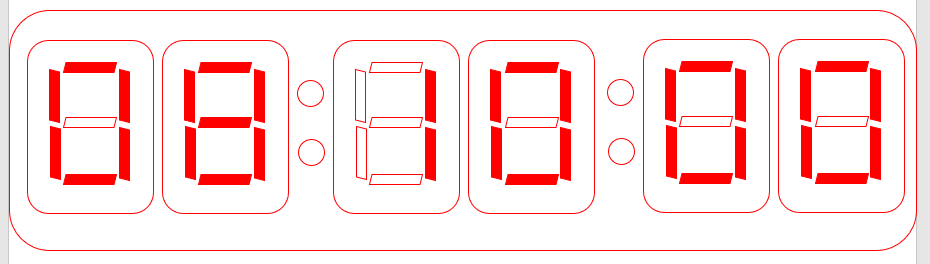
\includegraphics[width=5.90556in,height=1.67639in]{media/image45.png}

\subsection{TREINO}\label{treino-3}

\subsubsection{1}\label{section-51}

Analise o calendário a seguir.

\begin{longtable}[]{@{}l@{}}
\toprule
fevereiro 2023\tabularnewline
Dom\tabularnewline
\tabularnewline
5\tabularnewline
12\tabularnewline
19\tabularnewline
26\tabularnewline
\bottomrule
\end{longtable}

A última segunda-feira desse mês será o dia

\begin{quote}
A) 6.

B) 26.

C) 27.

D) 28.

SAEB: Identificar datas, dias da semana ou meses do ano em
calendário ou escrever uma data, apresentando o dia, o mês e o ano.
BNCC: EF01MA17 -- Reconhecer e relacionar períodos do dia, dias da semana
e meses do ano, utilizando calendário, quando necessário.

a) Incorreta. O aluno pode ter se confundido com a primeira segunda-feira.

b) Incorreta. O aluno pode ter se confundido com o domingo, entendendo que
a segunda-feira é o primeiro dia a aparecer no calendário.

c) Correta. Seguindo-se a coluna da segunda-feira (a segunda da esquerda para a direita), a última linha dessa coluna é a que contém o número 27.

d) Incorreta. O aluno pode ter confundido a segunda-feira com o último
dia do mês.
\end{quote}

\subsubsection{2}\label{section-52}

analise as figuras e indique qual é a sequência correta de
acontecimentos.

\textless{}https://br.freepik.com/vetores-gratis/antecedentes-da-paisagem-plana-em-tons-roxos\_1001699.htm\#query=anoitecer\&position=2\&from\_view=search\&track=sph;
https://br.freepik.com/vetores-gratis/paisagem-do-por-do-sol-com-lago-nuvens-no-ceu-vermelho-silhuetas-nas-colinas-e-arvores-na-costa\_12407808.htm\#query=amanhecer\&position=1\&from\_view=search\&track=sph

;
https://br.freepik.com/vetores-gratis/paisagem-de-primavera-desenhados-a-mao\_6804642.htm\#query=meio\%20dia\%20paisagem\&position=13\&from\_view=search\&track=ais

;
https://br.freepik.com/vetores-gratis/lua-cheia-noite-oceano-cartoon-ilustracao\_6690817.htm\#query=noite\%20paisagem\&position=10\&from\_view=search\&track=ais

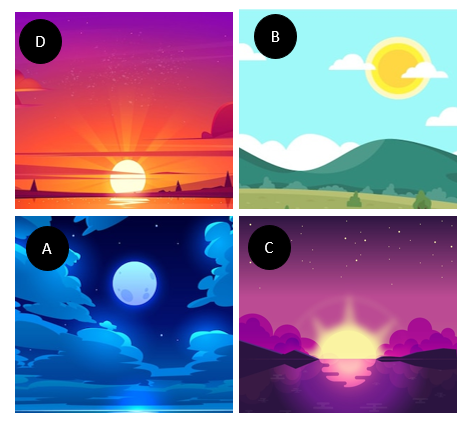
\includegraphics[width=4.85484in,height=4.39645in]{media/image46.png}

\begin{quote}
A) A, B, C, D.

B) B, A, C, D.

C) C, B, A, D.

D) D, B, C, A.

SAEB: Identificar sequência de acontecimentos relativos a um dia.
BNCC: EF01MA16 -- Relatar em linguagem verbal ou não verbal sequência de
acontecimentos relativos a um dia, utilizando, quando possível, os
horários dos eventos.

a) Incorreta. O aluno entendeu que deveria seguir a sequência das letras.

b) Incorreta. O aluno não considerou o amanhecer e foi direto ao dia.

c) Incorreta. O aluno pode ter confundido o entardecer com o amanhecer.

d) Correta. A sequência mostra o amanhecer, seguido do dia claro, seguido
do entardecer e seguido da noite estrelada.
\end{quote}

\subsubsection{3}\label{section-53}

Um balão levanta voô às 06:45 e volta ao chão às 07:45. qual é a duração
do voo?

\begin{quote}
A) 15 minutos.

B) 45 minutos.

C) 1 hora.

D) 1 hora e 45 minutos.

SAEB: Determinar o horário de início, o horário de término ou a
duração de um acontecimento.
BNCC: EF01MA16 -- Relatar em linguagem verbal ou não verbal sequência de
acontecimentos relativos a um dia, utilizando, quando possível, os
horários dos eventos.

a) Incorreta. O aluno só considerou os 15 minutos antes de
completar 7:00 horas.

b) Incorreta. O aluno esqueceu-se de considerar os 15 minutos antes de
completar 7:00 horas.

c) Correta. O aluno percebeu que o balão subiu no mesmo minuto em
que desceu, porém na hora posterior; logo o voo durou uma hora.

d) Incorreta. O aluno somou a hora aos 45 minutos.
\end{quote}

\section{5. MESADA}\label{muxf3dulo-5-quero-mesada}

Neste módulo, vamos desenvolver nos alunos a habilidade de reconhecerem o
valor das cédulas de dinheiro, assim como das moedas, por meio da
identificação de suas cores e dos próprios números que as representam.
Também vamos desenvolver nos alunos a capacidade de resolverem situações-problema que favorecem o trabalho com o tema contemporâneo transversal educação financeira.

Habilidade da BNCC
EF01MA19.

Habilidades do SAEB:

- Relacionar valores de moedas e/ou cédulas do sistema monetário
brasileiro, com base nas imagens desses objetos.

- Resolver problemas que envolvam moedas e/ou cédulas do sistema
monetário brasileiro.

\subsection{CONTEÚDO}\label{conteuxfado-4}

OBSERVE EStA TABELA, que
mostra as cédulas do dinheiro que usamos no brasil. o nome do nosso
dinheiro é \textbf{real} e o símbolo que o representa é este: \textbf{R\$}.

\textless{}referências das figuras das cédulas:
https://www.istockphoto.com/br/foto/brasileiro-dinheiro-novo-gm492403657-40519264;
https://www.istockphoto.com/br/foto/brasileiro-dinheiro-novo-gm492403659-40519468?phrase=5\%20REAIS;
https://www.istockphoto.com/br/foto/brasileiro-dinheiro-novo-gm492494099-40521892?phrase=10\%20REAIS;
https://www.istockphoto.com/br/foto/brasileiro-dinheiro-gm177321869-20141056?phrase=20\%20REAIS;
https://www.istockphoto.com/br/foto/brasileiro-dinheiro-gm147464521-20139849?phrase=50\%20REAIS;
https://www.istockphoto.com/br/foto/brasileiro-dinheiro-novo-gm492339651-40520246?phrase=100\%20REAIS;
https://www.istockphoto.com/br/foto/200-reais-bill-gm1285511748-382325664?phrase=200\%20REAIS.

\begin{longtable}[]{@{}llll@{}}
\toprule
IMAGEM & ANIMAL DESENHADO & COR DA CÉDULA & VALOR\tabularnewline
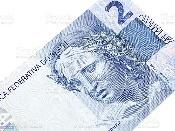
\includegraphics[width=0.79592in,height=0.59694in]{media/image47.jpg} &
TARTARUGA-MARINHA & AZUL & R\$ 2,00\tabularnewline
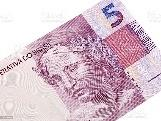
\includegraphics[width=0.73274in,height=0.54956in]{media/image48.jpg} &
GARÇA & ROSA & R\$ 5,00\tabularnewline
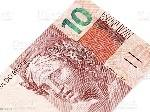
\includegraphics[width=0.68163in,height=0.51122in]{media/image49.jpg} &
ARARA VERMELHA & VERMELHA & R\$ 10,00\tabularnewline
\includegraphics[width=0.63139in,height=0.41990in]{media/image50.jpg} &
MICO-LEÃO-DOURADO & AMARELA & R\$ 20,00\tabularnewline
\includegraphics[width=0.63326in,height=0.42114in]{media/image51.jpg} &
ONÇA-PINTADA & LARANJA & R\$ 50,00\tabularnewline
\includegraphics[width=0.62794in,height=0.47095in]{media/image52.jpg} &
GAROUPA & AZUL & R\$ 100,00\tabularnewline
\includegraphics[width=0.63126in,height=0.42104in]{media/image53.jpg} &
LOBO-GUARÁ & BRANCA & R\$ 200,00\tabularnewline
\bottomrule
\end{longtable}

\coment{É importante que as crianças usem as peculiaridades de
cada cédula, como a cor predominante e o animal estampado, para
identificar o valor, além do número impresso. Se possível, mostre aos alunos cédulas
verdadeiras, com o intuito de lhes mostrar a marca d'água e outras
características que apontem para sua autenticidade.}

Agora, observe as moedas e perceba suas diferenças. A moeda de menor valor é a de 1 centavo, que representa um real dividido em 100 partes. A moeda de maior valor é a de 1 real, que equivale a cem centavos.

\textless{}https://br.freepik.com/fotos-gratis/dinheiro-moedas-brasileiras-escada\_23076933.htm\#page=9\&query=REAIS\%20moedas\&position=39\&from\_view=search\&track=ais\textgreater{}

\includegraphics[width=5.90556in,height=1.41667in]{media/image54.jpg}\protect\hypertarget{_heading=h.eii4svey01jf}{}{}

\subsection{ATIVIDADES}\label{atividades-4}

\subsubsection{1}\label{section-54}

marque, na etiqueta, o valor de cada produto.

\textless{}https://br.freepik.com/vetores-gratis/colecao-de-brinquedos-de-natal-desenhada-a-mao\_11105919.htm\#query=brinquedos\%20com\%20etiquetas\&position=14\&from\_view=search\&track=ais.
Inserir na coluna da direita uma figura de etiqueta para o aluno
preencher o valor da mercadoria.\textgreater{}

\begin{longtable}[]{@{}lll@{}}
\toprule
\includegraphics[width=1.70857in,height=2.10446in]{media/image55.png} &
Cento e trinta e cinco reais e vinte centavos. &
\includegraphics[width=2.19822in,height=2.44826in]{media/image56.png}\tabularnewline
\bottomrule
\end{longtable}

R\$ 135,20.

\begin{longtable}[]{@{}lll@{}}
\toprule
\includegraphics[width=1.16683in,height=1.08348in]{media/image57.png} &
cinquenta e cinco reais e vinte e cinco centavos. &
\includegraphics[width=2.19822in,height=2.44826in]{media/image56.png}\tabularnewline
\bottomrule
\end{longtable}

R\$ 55,25.

\begin{longtable}[]{@{}lll@{}}
\toprule
\includegraphics[width=1.96902in,height=1.29185in]{media/image58.png} &
noventa e oito reais. &
\includegraphics[width=2.19822in,height=2.44826in]{media/image56.png}\tabularnewline
\bottomrule
\end{longtable}

R\$ 98,00.

\begin{longtable}[]{@{}lll@{}}
\toprule
\includegraphics[width=1.60439in,height=1.38561in]{media/image59.png} &
quarenta e dois reais e noventa e nove centavos. &
\includegraphics[width=2.19822in,height=2.44826in]{media/image56.png}\tabularnewline
\bottomrule
\end{longtable}

R\$ 42,99.

\subsubsection{2}\label{section-55}

escreva por extenso os valores em reais.

\textless{}Inserir a tabela conforme o modelo abaixo\textgreater{}

\begin{longtable}[]{@{}ll@{}}
\toprule
R\$ 135,60 & Cento e trinta e cinco reais e sessenta
centavos.\tabularnewline
R\$ 465,00 & Quatrocentos e sessenta e cinco reais.\tabularnewline
R\$ 59,30 & Cinquenta e nove reais e trinta centavos.\tabularnewline
R\$ 74,15 & Setenta e quatro reais e quinze centavos.\tabularnewline
R\$ 63,20 & Sessenta e três reais e vinte centavos.\tabularnewline
R\$ 15,15 & Quinze reais e quinze centavos.\tabularnewline
\bottomrule
\end{longtable}


\subsubsection{3}\label{section-56}

ligue corretamente cada valor a uma imagem.

\textless{}https://br.freepik.com/fotos-gratis/dinheiro-moedas-brasileiras-1-real\_22809605.htm\#query=moeda\%20de\%201\%20real\%20dineiro\%20barssileiro\&position=1\&from\_view=search\&track=ais;
https://br.freepik.com/fotos-gratis/dinheiro-moedas-brasileiras-5-centavos\_22781620.htm\#query=moeda\%20de\%205\%20centavos\%20dineiro\%20barssileiro\&position=2\&from\_view=search\&track=ais;
https://br.freepik.com/fotos-gratis/dinheiro-moedas-brasileiras-10-centavos\_22781622.htm\#query=moeda\%20de\%2010\%20centavos\%20dineiro\%20barssileiro\&position=6\&from\_view=search\&track=ais;

\begin{longtable}[]{@{}ll@{}}
\toprule
R\$ 0,05 &
\includegraphics[width=0.80577in,height=0.79447in]{media/image60.jpg}\tabularnewline
R\$ 0,50 &
\includegraphics[width=0.69145in,height=0.53632in]{media/image61.jpg}\tabularnewline
R\$ 0,25 &
\includegraphics[width=0.75523in,height=0.67928in]{media/image62.jpg}\tabularnewline
R\$ 0,10 &
\includegraphics[width=0.67617in,height=0.63139in]{media/image63.jpg}\tabularnewline
R\$ 1,00 &
\includegraphics[width=0.69044in,height=0.66964in]{media/image64.jpg}\tabularnewline
\bottomrule
\end{longtable}

Se os alunos tiverem alguma dificuldade com esta atividade,
uma vez que ainda não tiveram contato com números fracionários, ajude-os
a associarem os valores às imagens das moedas.

\subsubsection{4}\label{section-57}

preencha cada espaço com a quantidade de cédulas necessárias para comprar o item correspondente. Use somente cédulas.

\textless{}https://www.istockphoto.com/br/foto/notas-de-dinheiro-do-brasil-em-composto-detalhes-de-notas-de-200-50-10-5-e-2-reais-gm1280319451-378658163?phrase=200\%20REAIS.
Inserir quadros para que os alunos consigam colocar a quantidade de
notas necessárias.\textgreater{}

\begin{enumerate}
\def\labelenumi{\Alph{enumi})}
\item
  um carrinho de r\$ 100,00.
\end{enumerate}

\includegraphics[width=5.90556in,height=2.19028in]{media/image65.png}

\begin{enumerate}
\def\labelenumi{\Alph{enumi})}
\item
  uma boneca de R\$ 70,00.
\end{enumerate}

\includegraphics[width=5.90556in,height=2.18611in]{media/image66.png}

\begin{enumerate}
\def\labelenumi{\Alph{enumi})}
\item
  uma calça de R\$ 137,00.
\end{enumerate}

\includegraphics[width=5.90556in,height=2.12778in]{media/image67.png}

\begin{enumerate}
\def\labelenumi{\Alph{enumi})}
\item
  uma saia de R\$ 85,00.
\end{enumerate}

\includegraphics[width=5.90556in,height=2.18056in]{media/image68.png}

\begin{enumerate}
\def\labelenumi{\Alph{enumi})}
\item
  um chocolate de R\$ 6,00.
\end{enumerate}

\includegraphics[width=5.90556in,height=2.14583in]{media/image69.png}

\begin{enumerate}
\def\labelenumi{\Alph{enumi})}
\item
  Um par de óculos escuros de R\$ 450,00.
\end{enumerate}

\includegraphics[width=5.90556in,height=2.19931in]{media/image70.png}

Exceto para o chocolate, de R\$ 6,00, há mais de uma combinação possível para cada item. É de suma importância
trabalhar com os alunos as respostas diferentes.

\subsubsection{5}\label{section-58}

preencha cada círcula com a quantidade de moedas necessárias para comprar o item correspondente. Use somente moedas.

\begin{quote}
\textless{}https://br.freepik.com/fotos-gratis/dinheiro-moedas-brasileiras-escada\_23076933.htm\#page=9\&query=REAIS\%20moedas\&position=39\&from\_view=search\&track=ais.
Inserir os círculos abaixo de cada moeda para o aluno preencher a
quantidade necessária.\textgreater{}
\end{quote}

\begin{enumerate}
\def\labelenumi{\Alph{enumi})}
\item
  um pirulito de R\$ 0,35 (trinta e cinco centavos).
\end{enumerate}

\includegraphics[width=4.34436in,height=1.66690in]{media/image71.png}

\begin{enumerate}
\def\labelenumi{\Alph{enumi})}
\item
  uma bala de R\$ 0,15 (quinze centavos).
\end{enumerate}

\includegraphics[width=4.41728in,height=1.68774in]{media/image72.png}

\begin{enumerate}
\def\labelenumi{\Alph{enumi})}
\item
  Um apito de R\$ 0,30 (trinta centavos).
\end{enumerate}

\includegraphics[width=4.35477in,height=1.63565in]{media/image73.png}

\begin{enumerate}
\def\labelenumi{\Alph{enumi})}
\item
  um chaveiro de super-herói de r\$ 3,75 (três reais e setenta e cinco
  centavos).
\end{enumerate}

\includegraphics[width=4.39645in,height=1.81275in]{media/image74.png}

Os alunos precisarão de uma ajuda extra por não conhecerem números fracionários.

\subsubsection{6}\label{section-59}

João e bianca ganharam R\$ 10,00 (cada um). joão comprou um doce de R\$ 6,00,
e bianca comprou um doce de R\$ 5,00. Sobre essa situação, responda ao que se pergunta a seguir.

\begin{enumerate}
\def\labelenumi{\Alph{enumi})}
\item
  quanto joão e bianca ganharam juntos? Responda com algarismos e por extenso.
\end{enumerate}

\textless{}2 linhas\textgreater{}

R\$ 10,00 + R\$ 10,00 = R\$ 20,00 -- vinte reais.

\begin{enumerate}
\def\labelenumi{\Alph{enumi})}
\item
  Quanto joão e bianca gastaram juntos?
\end{enumerate}

\textless{}2 linhas\textgreater{}

R\$ 6,00 + R\$ 5,00 = R\$ 11,00 -- onze reais.

\begin{enumerate}
\def\labelenumi{\Alph{enumi})}
\item
  quanto dinheiro sobrou para joão e bianca juntos?
\end{enumerate}

\textless{}2 linhas\textgreater{}

R\$ 20,00 -- R\$ 11,00 = R\$ 9,00 -- nove reais.

\begin{enumerate}
\def\labelenumi{\arabic{enumi}.}
\item
  desenhe, inclusive com cores, as cédulas e as moedas do real. tente se lembrar do maior número possível de detalhes de cada uma.
\end{enumerate}

\textless{} Inserir um quadro que tome toda uma página, para que os
alunos desenhem as cédulas e moedas.\textgreater{}


\subsection{TREINO}\label{treino-4}

\subsubsection{1}\label{section-60}

Observe a imagem a seguir.

\textless{}https://www.istockphoto.com/br/foto/brasileiro-dinheiro-novo-gm492494099-40521892?phrase=10\%20REAIS\textgreater{}

O valor da cédula representada na imagem é de

\includegraphics[width=1.92157in,height=1.43284in]{media/image75.png}

A) R\$ 0,10.

B) R\$ 1,00.

C) R\$ 10,00.

D) R\$ 100,00.

SAEB: Relacionar valores de moedas e/ou cédulas do sistema
monetário brasileiro, com base nas imagens desses objetos.
BNCC: EF01MA19 -- Reconhecer e relacionar valores de moedas e cédulas do
sistema monetário brasileiro para resolver situações simples do
cotidiano do estudante.

a) Incorreta. O aluno confundiu a cédula de 10 reais com uma moeda de 10 centavos.

b) Incorreta. O aluno confundiu a cédula de 10 reais com uma moeda de 1 real.

c) Correta. A cédula representada é a de 10 reais.

d) Incorreta. O aluno confundiu a cédula de 10 reais com outra cédula, a de 100 reais.

\subsubsection{2}\label{section-61}

Cristiano comprou um chapéu de R\$ 75,00. De que forma ele pode ter pagado por esse chapéu?

A) com duas cédulas de R\$ 50,00.

B) com três cédulas de R\$ 25,00.

C) com três cédulas de r\$ 10,00.

D) com três cédulas de R\$ 5,00.

SAEB: Resolver problemas que envolvam moedas e/ou cédulas do
sistema monetário brasileiro.
BNCC: EF01MA19 -- Reconhecer e relacionar valores de moedas e cédulas do
sistema monetário brasileiro para resolver situações simples do
cotidiano do estudante.

a) Correta. A composição resulta em 100 reais, valor suficiente para pagar pelo chapéu.

b) Incorreta. Apesar de a composição resultar em 75 reais, o valor do chapéu, não existe cédula de 25 reais.

c) Incorreta. A composição resulta em R\$ 30,00, valor insuficiente para pagar pelo chapéu.

d) Incorreta. A composição resulta em R\$ 15,00, valor insuficiente para pagar pelo chapéu.

\subsubsection{3}\label{section-62}

Ana precisa pagar uma fatura de R\$ 182,00. Ela está com uma cédula de R\$ 100,00, uma cédula de R\$ 50,00, uma cédula de R\$ 20,00 e duas cédulas de R\$ 5,00. Pode-se afirmar que Ana

A) tem o valor exato para pagar a fatura.

B) consegue completar o valor com uma moeda só.

C) precisa ter pelo menos mais uma cédula de R\$ 2,00.

D) continuaria sem o valor certo mesmo com mais uma cédula de R\$ 5,00.

SAEB: Resolver problemas que envolvam moedas e/ou cédulas do
sistema monetário brasileiro.
BNCC: EF01MA19 -- Reconhecer e relacionar valores de moedas e cédulas do
sistema monetário brasileiro para resolver situações simples do
cotidiano do estudante.

a) Incorreta. Ana tem R\$ 180,00, valor que não é suficiente para pagar a fatura de R\$ 182,00.

b) Incorreta. Não existe uma moeda de R\$ 2,00 para completar o valor necessário para pagar a fatura.

c) Correta. Ana tem R\$ 180,00 e, com mais uma cédula de R\$ 2,00, completaria o valor para pagar a fatura.

d) Incorreta. Com mais uma cédula de R\$ 5,00, Ana teria R\$ 185,00, valor mais que suficiente para pagar a fatura de R\$ 182,00.

\section{6. SERÁ QUE VAI
CHOVER?}\label{muxf3dulo-6-seruxe1-que-vai-chover}

Neste módulo, vamos trabalhar a habilidade dos alunos de
perceber que alguns fatos podem ser previsíveis, e outros não. A
noção de probabilidade matemática pode ser um pouco complexa para
crianças da idade, porém, com situações do cotidiano, pode-se fazer com que elas percebam que é mais provável que isto ou aquilo aconteça.

Habilidade do SAEB:

- Classificar resultados de eventos cotidianos aleatórios como ``pouco
prováveis'', ``muito prováveis'', ``certos'' ou ``impossíveis''.

Habilidade da BNCC
EF01MA20.

\subsection{CONTEÚDO}\label{conteuxfado-5}

Como é possivel saber se vai chover ou não? existe toda uma ciência por trás dessa previsão: a meteorologia.
No entanto, se olhamos para o céu e o vemos escuro, criamos a expectativa de vai chover, mesmo sem usar uma ciência mais precisa. Na meteorologia, uma série de acontecimentos
permite aos técnicos fazer uma previsão do tempo, mas nós também podemos fazer previsões no dia a dia. Podemos dizer que existem quatro possibilidades. Por exemplo:

\textless{}Inserir um quadro conforme o modelo a seguir, utilizando as
referências:
https://br.freepik.com/vetores-premium/pequeno-elefante-voar-para-o-ceu\_6579577.htm\#query=elefante\%20voando\&position=9\&from\_view=search\&track=ais;
https://br.freepik.com/vetores-gratis/fundo-plano-do-polo-norte-da-temporada-de-inverno\_33138109.htm\#query=neve\&position=11\&from\_view=search\&track=sph
(alterar a placa colocando nela Brasil no lugar de polo norte.;
https://br.freepik.com/vetores-gratis/ilustracao-de-calor-de-verao-plana-com-homem-na-cadeira\_27995494.htm\#query=ver\%C3\%A3o\%20calor\&position=0\&from\_view=search\&track=ais;
https://br.freepik.com/vetores-premium/jogador-de-futebol-jogando-futebol-em-pe\_33803714.htm\#query=bola\%20jogada\%20pra\%20cima\&position=7\&from\_view=search\&track=ais.\textgreater{}

\begin{longtable}[]{@{}llll@{}}
\toprule
impossível & quando não existe a menor chance de algo acontecer & um
elefante sair voando por conta própria &
\includegraphics[width=1.42708in,height=1.42708in]{media/image76.jpg}\tabularnewline
pouco provável & quando existe uma pequena chance de algo acontecer &
nevar no brasil &
\includegraphics[width=1.52602in,height=1.01167in]{media/image77.png}\tabularnewline
muito provável & quando existe uma grande chance de algo acontecer &
fazer calor no verão &
\includegraphics[width=1.30208in,height=1.30208in]{media/image78.jpg}\tabularnewline
certeza & quando é certo que algo vai acontecer & uma bola cair quando
for jogada para cima &
\includegraphics[width=1.04437in,height=1.39696in]{media/image79.jpg}\tabularnewline
\bottomrule
\end{longtable}

É importante ressaltar com os alunos que, no Brasil, é raro
nevar, mas pode acontecer, principalmente na região Sul. Vale
ressaltar também que nem todos os dias do verão são quentes, ou seja, a
temperatura pode cair em alguns dias.

\subsection{ATIVIDADES}\label{atividades-5}

\subsubsection{1}\label{section-63}

pinte os círculos com as situações impossíveis no quadro a seguir. pinte
da cor que você preferir.

\textless{}criar um quadro com as situações descritas conforme o modelo
a seguir.\textgreater{}

\includegraphics[width=5.16074in,height=7.09420in]{media/image80.png}

Esta atividade pode ser importante para trabalhar a
habilidade de leitura dos alunos. As situações impossíveis são: céu
ficando verde, tesoura falando, jacaré voando, leão miando, unicórnios existindo,
chuva caindo para cima e árvore andando.

\subsubsection{2}\label{section-64}

nos quadros a seguir, desenhe duas situações que você considere
impossíveis. não repita as situações da atividade anterior consideradas impossíveis.

\textless{}Inserir dois quadros para os alunos desenharem, tomando toda
a página\textgreater{}

\includegraphics[width=4.38938in,height=7.65199in]{media/image81.png}

Permita que os alunos utilizem a
imaginação sem moderação. Começar com os acontecimentos
impossíveis é importante, pois permite que o aluno utilize sua
imaginação, provocando engajamento e envolvimento na criança.

\subsubsection{3}\label{section-65}

ligue cada situação com a imagem correspondente.

\textless{}https://br.freepik.com/vetores-gratis/chovendo-na-natureza-paisagem\_5769787.htm\#query=rel\%C3\%A3mpago\%20na\%20chuva\&position=6\&from\_view=search\&track=ais;
https://br.freepik.com/vetores-gratis/tartaruga-jogando-skate-no-parque\_4119896.htm\#query=sapo\%20jogando\%20volei\&position=0\&from\_view=search\&track=ais;

\begin{longtable}[]{@{}ll@{}}
\toprule
\begin{minipage}[t]{0.48\columnwidth}\raggedright\strut
\includegraphics[width=2.03487in,height=1.82023in]{media/image82.jpg}

relampejar na chuva\strut
\end{minipage} & \begin{minipage}[t]{0.48\columnwidth}\raggedright\strut
impossível\strut
\end{minipage}\tabularnewline
\begin{minipage}[t]{0.48\columnwidth}\raggedright\strut
\includegraphics[width=2.11035in,height=1.45968in]{media/image83.jpg}

tartaruga \textit{skatista}\strut
\end{minipage} & \begin{minipage}[t]{0.48\columnwidth}\raggedright\strut
pouco provável\strut
\end{minipage}\tabularnewline
\begin{minipage}[t]{0.48\columnwidth}\raggedright\strut
\includegraphics[width=2.11129in,height=1.37616in]{media/image84.jpg}

acidente aéreo\strut
\end{minipage} & \begin{minipage}[t]{0.48\columnwidth}\raggedright\strut
muito provável\strut
\end{minipage}\tabularnewline
\begin{minipage}[t]{0.48\columnwidth}\raggedright\strut
\includegraphics[width=1.86458in,height=1.86458in]{media/image85.jpg}

sentir fome\strut
\end{minipage} & \begin{minipage}[t]{0.48\columnwidth}\raggedright\strut
certo\strut
\end{minipage}\tabularnewline
\bottomrule
\end{longtable}

\subsubsection{4}\label{section-66}

preencha com um x as possibilidades do quadro a seguir.

\begin{longtable}[]{@{}lllll@{}}
\toprule
situação & impossível & pouco provável & muito provável &
certa\tabularnewline
esquecer-se de escovar os dentes & & & &\tabularnewline
esquecer-se de fazer a lição & & & &\tabularnewline
jogar \textit{videogame} todo o dia & & & &\tabularnewline
sentir vontade de ir ao banheiro & & & &\tabularnewline
brincar com um adulto & & & &\tabularnewline
brincar com outra criança & & & &\tabularnewline
receber um amigo em casa & & & &\tabularnewline
esquecer a luz acesa & & & &\tabularnewline
esquecer-se de dar a descarga depois de usar o banheiro & & &
&\tabularnewline
comer doces fora de hora & & & &\tabularnewline
assitir à tv ou ficar na internet na hora de comer & & & &\tabularnewline
\bottomrule
\end{longtable}

Com esta atividade, pode-se auxiliar o aluno a fazer uma autoavaliação de como ele administra seu tempo diariamente, além de ajudá-lo
a criar suas prioridades. A atividade favorece o trabalho com os temas contemporâneos transversair sáude e vida familiar e social.

\subsubsection{5}\label{section-67}

zélia estava brincando de jogar um dado. No quadro a seguir, pinte quais são
os resultados prováveis de saírem quando zélia jogar uma vez.

\begin{longtable}[]{@{}llll@{}}
\toprule
\includegraphics[width=1.55208in,height=1.55208in]{media/image86.jpg} &
1 & 15 & 6\tabularnewline
& 20 & 3 & 8\tabularnewline
& 5 & 10 & 9\tabularnewline
& 11 & 4 & 12\tabularnewline
& 13 & 14 & 2\tabularnewline
\bottomrule
\end{longtable}

Espera-se que os alunos percebram que só podem sair os
resultados de 1 a 6, visto que são os únicos números que há em um
dado. Se possível, mostre um dado para os alunos durante a
atividade.

\subsubsection{6}\label{section-68}

DESCUBRA QUAL DOS JOGADORES A SEGUIR TEM A MAIOR CHANCE DE GANHAR O JOGO
DE DOMINÓS. CIRCULE O NOME DESSE JOGADOR.

\textless{}https://br.freepik.com/vetores-gratis/ilustracao-realista-de-jogo-de-domino\_22656073.htm\#query=domin\%C3\%B3\%20jogada\&position=29\&from\_view=search\&track=ais;
https://br.freepik.com/vetores-premium/stock-vector-domino-conjunto-completo-ilustracao-realista-colecao-de-cartoes-de-domino-de-cor-preto-e-branco\_22221437.htm\#query=domin\%C3\%B3\%20jogada\&position=35\&from\_view=search\&track=ais\textgreater{}

\includegraphics[width=4.84499in,height=2.71476in]{media/image87.png}

Solange é a única
jogadora que possui uma pedra com o número 5. Nenhum outro jogador
possui uma pedra assim; logo a chance de vitória de Solange é maior.

\subsubsection{7}\label{section-69}

bernardo está brincando de colocar diferentes tipos de bola na água
para ver qual flutua. você consegue prever qual será o resultado? assinale
com um x.

\textless{}Inserir quadro conforme o modelo a seguir, utilizando as
referências:
https://br.freepik.com/fotos-premium/bola-de-papel-amassado\_25578632.htm?query=bola\%20de\%20papel\#from\_view=detail\_alsolike
https://br.freepik.com/vetores-premium/bola-de-cromo-3d-realista-isolada-no-fundo-branco\_34098681.htm\#query=bola\%20de\%20metal\&position=24\&from\_view=search\&track=ais;
https://br.freepik.com/vetores-premium/esfera-branca-bola-ilustracao\_9402860.htm\#query=bola\%20de\%20isopor\&position=13\&from\_view=search\&track=ais;
https://br.freepik.com/vetores-premium/bola-de-bilhar\_26468289.htm\#query=bola\%20de\%20bilhar\&position=46\&from\_view=search\&track=ais
\textgreater{}

\begin{longtable}[]{@{}llll@{}}
\toprule
\begin{minipage}[t]{0.24\columnwidth}\raggedright\strut
\includegraphics[width=1.06165in,height=0.99037in]{media/image88.jpg}

Bola de papel flutua?\strut
\end{minipage} & \begin{minipage}[t]{0.24\columnwidth}\raggedright\strut
\includegraphics[width=0.98125in,height=0.98125in]{media/image89.jpg}

Bola de metal flutua?\strut
\end{minipage} & \begin{minipage}[t]{0.24\columnwidth}\raggedright\strut
\includegraphics[width=0.83333in,height=0.83333in]{media/image90.jpg}

Bola de isopor flutua?\strut
\end{minipage} & \begin{minipage}[t]{0.24\columnwidth}\raggedright\strut
\includegraphics[width=0.83333in,height=0.83333in]{media/image91.jpg}

Bola de bilhar flutua?\strut
\end{minipage}\tabularnewline
sim & & sim &\tabularnewline
não & & não &\tabularnewline
talvez & & talvez &\tabularnewline
\bottomrule
\end{longtable}

Ainda que os alunos não conheçam o
conceito de flutuabilidade, é importante
desenvolver suas habilidades de prever um acontecimento, baseando-se no
senso comum ou até em experiências pessoais. Alguns alunos podem ter
manipulado algumas dessas bolas ou feito alguma experiência
desse tipo. Se julgar necessário, se for possível, faça a experiência em
sala de aula. Você pode promover um jogo de adivinhação, promovendo
maior engajamento dos alunos. Não é viável entrar no conceito de
densidade por ser um assunto muito complexo para a idade, porém deve-se
tomar cuidado para não criar um subsunçor na estrutura cognitiva do
aluno acerca da massa das bolas como se fosse o fator determinante para a
flutuação.

\subsubsection{8}\label{section-70}

discuta uma situação com os colegas que seja muito provável e desenhe
essa situação no quadro a seguir. depois, descreva que situação é essa.

\textless{}Inserir um quadro para o aluno desenhar além de seis linhas
para o aluno descrever a situação. Essa atividade deve preencher uma
página\textgreater{}

\includegraphics[width=3.24914in,height=2.92171in]{media/image92.png}

Aproveite a atividade para desenvolver a habilidade de
escrita. Oriente os alunos quanto à escolha da situação.

\subsubsection{9}\label{section-71}

discuta uma situação com os colegas que seja pouco provável e desenhe
essa situação no quadro a seguir. depois, descreva que situação é essa.

\textless{}Inserir um quadro para o aluno desenhar além de seis linhas
para o aluno descrever a situação. Essa atividade deve preencher uma
página\textgreater{}

\includegraphics[width=2.86272in,height=2.57423in]{media/image92.png}


\subsubsection{10}\label{section-72}

discuta uma situação com os colegas que seja certa (ou seja, que represente uma certeza) e desenhe essa
situação no quadro a seguir, depois, descreva que situação é essa.

\textless{}Inserir um quadro para o aluno desenhar além de seis linhas
para o aluno descrever a situação. Essa atividade deve preencher uma
página\textgreater{}

\includegraphics[width=2.86272in,height=2.57423in]{media/image92.png}


\subsection{TREINO}\label{treino-5}

\subsubsection{1}\label{section-73}

Uma situação impossível de acontecer é

A) uma caneta escrever.

B) um gato dormir.

C) um navio flutuar.

D) um peixe cantar.

SAEB: Classificar resultados de eventos cotidianos aleatórios como
``pouco prováveis'', ``muito prováveis'', ``certos'' ou ``impossíveis''.
BNCC: EF01MA20 -- Classificar eventos envolvendo o acaso, tais como
``acontecerá com certeza'', ``talvez aconteça'' e ``é impossível
acontecer'', em situações do cotidiano.

a) Incorreta. Uma caneta é feita para escrever.

b) Incorreta. Gatos também dormem.

c) Incorreta. Todo navio foi feito para flutuar.

d) Correta. Peixes não podem cantar.

\subsubsection{02}\label{section-74}

Indique qual destas situações é pouco provável de acontecer.

A) fazer calor no verão.

B) fazer frio no verão.

C) nevar no inverno.

D) surgirem flores na primavera.

SAEB: Classificar resultados de eventos cotidianos aleatórios como
``pouco prováveis'', ``muito prováveis'', ``certos'' ou ``impossíveis''.
BNCC: EF01MA20 -- Classificar eventos envolvendo o acaso, tais como
``acontecerá com certeza'', ``talvez aconteça'' e ``é impossível
acontecer'', em situações do cotidiano.

a) Incorreta. É muito provável que faça calor no verão.

b) Correta. É pouco provável que faça frio no verão, ainda que seja
possível.

c) Incorreta. É muito provável que neve caia no inverno, principalmente
no hemisfério Norte do planeta.

d) Incorreta. É certeza que as árvores florescem na primavera.

\subsubsection{3}\label{section-75}

Analise esta imagem.

Inserir imagem: https://br.freepik.com/fotos-gratis/bela-vista-de-uma-estrada-vazia-cercada-por-vegetacao-sob-nuvens-escuras-de-tempestade_17110244.htm#query=tempo%20nublado&position=1&from_view=search&track=ais

O que se pode afirmar sobre a possibilidade de chuva na região retratada na imagem?

A) É impossível que chova.

B) É certo que chova.

C) É pouco provável que chova.

D) É muito provável que chova.

SAEB: Classificar
resultados de eventos cotidianos aleatórios como ``pouco prováveis'',
``muito prováveis'', ``certos'' ou ``impossíveis''.
BNCC: EF01MA20 -- Classificar eventos envolvendo o acaso, tais como
``acontecerá com certeza'', ``talvez aconteça'' e ``é impossível
acontecer'', em situações do cotidiano.

a) Incorreta. É sempre possível que chova em alguma lugar.

b) Incorreta. Sempre existe a chance de não chover, apesar do tempo fechado.

c) Incorreta. Como o tempo está bem fechado na cena retratada, é muito provável que chova.

d) Correta. O tempo bem fechado indica que a probabilidade de chuva é bem grande.

\section{7. TUDO
ORGANIZADINHO}\label{muxf3dulo-7-tudo-organizadinho}

Neste módulo, vamos desenvolver nos alunos a habilidade de identificar e
colocar informações em gráficos e tabelas.

Habilidades do SAEB:
- Ler/identificar ou comparar dados estatísticos ou informações,
expressos em tabelas (simples ou de dupla entrada).
- Ler/identificar ou comparar dados estatísticos expressos em gráficos
(barras simples, colunas simples ou pictóricos).
- Representar os dados de uma pesquisa estatística ou de um levantamento
em listas, tabelas (simples ou de dupla entrada) ou gráficos (barras
simples, colunas simples ou pictóricos).

Habilidades da BNCC
EF01MA21, EF01MA22.

\subsection{CONTEÚDO}\label{conteuxfado-6}

você já percebeu como listas
de compras, listas de materiais da escola ou então o
\emph{ranking} de um jogo ficam organizados? Eles ficam organizados em estruturas que chamamos de \textbf{tabela}. Observe:

\textless{}Inserir a referência:
https://br.freepik.com/vetores-gratis/tabela-de-classificacao-com-fundo-abstrato\_11187227.htm\#query=score\%20game\&position=0\&from\_view=search\&track=ais.
Não é necessário traduzir. Os alunos estão habituados a \emph{games} e
suas terminologias nessa idade.\textgreater{}

\includegraphics[width=1.77083in,height=1.77083in]{media/image93.jpg}

a classificação e os pontos dos jogadores desse jogo são apresentados em
uma tabela. como temos duas informações, ou seja, a classificação e a
pontuação, dizemos que se trata de uma \textbf{tabela de dupla entrada}.

Outro modo de organizar informações são os \textbf{gráficos}. Veja:

\textless{}Criar gráficos conforme o modelo a seguir.\textgreater{}

{{[}CHART{]}}\includegraphics[width=3.13415in,height=1.79094in]{media/image94.png}

Em uma escola, perguntaram para que time os alunos de uma turma torciam. o
resultado está nesses gráficos. perceba que a maioria das crianças
torcia para o Sabático. os gráficos ajudam a perceber isso mais facilmente. Você saberia dizer, só olhando para eles, qual time foi o menos escolhido?

\subsection{ATIVIDADES}\label{atividades-6}

\subsubsection{1}\label{section-76}

analise a tabela, que mostra a pontuação de jogadores em uma partida de
boliche.

\textless{}Inserir tabela conforme o modelo a seguir. Inserir a
referência:
https://br.freepik.com/vetores-premium/jogador-de-boliche\_2938032.htm\#query=boliche\%20crian\%C3\%A7as\&position=5\&from\_view=search\&track=ais.\textgreater{}

\includegraphics[width=1.88542in,height=1.88542in]{media/image95.jpg}

\begin{longtable}[]{@{}ll@{}}
\toprule
jogador & pontuação\tabularnewline
\midrule
\endhead
marcos & 46\tabularnewline
ricardo & 56\tabularnewline
suzana & 32\tabularnewline
hévilin & 31\tabularnewline
débora & 47\tabularnewline
lucas & 35\tabularnewline
marcelo & 35\tabularnewline
\bottomrule
\end{longtable}

Agora, responda ao que se pergunta a seguir.

\begin{enumerate}
\def\labelenumi{\Alph{enumi})}
\item
  quem fez mais pontos?
\end{enumerate}

\textless{}1 linha\textgreater{}

Ricardo tem a maior pontuação.

\begin{enumerate}
\def\labelenumi{\Alph{enumi})}
\item
  quem fez menos pontos?
\end{enumerate}

\textless{}1 linha\textgreater{}

Hévilin tem a menor pontuação.

\begin{enumerate}
\def\labelenumi{\Alph{enumi})}
\item
  houve algum empate?
\end{enumerate}

\textless{}1 Linha\textgreater{}

Lucas e Marcelo empataram com 35 pontos.

\begin{enumerate}
\def\labelenumi{\Alph{enumi})}
\item
  Quem são os três primeiros colados ao final da partida?
\end{enumerate}

\textless{}1 Linha\textgreater{}

Ricardo (1º), Débora (2º) e Marcos (3º).

\subsubsection{02}\label{section-77}

Em uma turma de primeiro ano, foi feita uma pesquisa para saber que tipo de alimento as
crianças mais comiam. o resultado está representado no grÁfico a seguir. Analise-o.

\textless{}Inserir gráfico conforme o modelo a seguir.\textgreater{}

{{[}CHART{]}}

Agora, responda ao que se pergunta a seguir?

\begin{enumerate}
\def\labelenumi{\Alph{enumi})}
\item
  qual é a comida preferida dessa turma?
\end{enumerate}

\textless{}1 linha\textgreater{}

A maioria dos alunos prefere massa.

\begin{enumerate}
\def\labelenumi{\Alph{enumi})}
\item
  qual é a comida menos querida dessa turma?
\end{enumerate}

\textless{}1 linha\textgreater{}

A minoria dos alunos costuma comer verduras.

\begin{enumerate}
\def\labelenumi{\Alph{enumi})}
\item
  qual é a segunda comida preferida dos alunos dessa turma?
\end{enumerate}

\textless{}1 Linha\textgreater{}

Doces são a segunda comida preferida dos alunos.

\begin{enumerate}
\def\labelenumi{\Alph{enumi})}
\item
  Qual das comidas você teria escolhido como a sua favorita? Por quê?
\end{enumerate}

\textless{}3 linhas\textgreater{}

Resposta pessoal.

\subsubsection{3}\label{section-78}

a tabela a seguir mostra a lista dos jogos mais jogados e mais curtidos pelos
alunos de uma turma de primeiro ano. A tabela também mostra quantos alunos preferem cada
jogo.

\begin{longtable}[]{@{}ll@{}}
\toprule
\emph{minecraft} & 8\tabularnewline
\emph{mario kart 8} & 9\tabularnewline
\emph{animal crossing: new horizons} & 5\tabularnewline
\emph{super mario party} & 3\tabularnewline
\emph{roblox} & 10\tabularnewline
\bottomrule
\end{longtable}

\begin{enumerate}
\def\labelenumi{\Alph{enumi})}
\item
  Na tabela a seguir, coloque os jogos em ordem do
  mais jogado para o menos jogado.
\end{enumerate}

\begin{longtable}[]{@{}ll@{}}
\toprule
\emph{minecraft} & 3\tabularnewline
\emph{mario kart 8} & 2\tabularnewline
\emph{animal crossing: new horizons} & 4\tabularnewline
\emph{super mario party} & 5\tabularnewline
\emph{roblox} & 1\tabularnewline
\bottomrule
\end{longtable}


\begin{enumerate}
\def\labelenumi{\Alph{enumi})}
\item
  preencha o gráfico a seguir, pintando os quadradinhos conforme a tabela
  de alunos.
\end{enumerate}

\begin{longtable}[]{@{}llllll@{}}
\toprule
10 & & & & &\tabularnewline
9 & & & & &\tabularnewline
8 & & & & &\tabularnewline
7 & & & & &\tabularnewline
6 & & & & &\tabularnewline
5 & & & & &\tabularnewline
4 & & & & &\tabularnewline
3 & & & & &\tabularnewline
2 & & & & &\tabularnewline
1 & & & & &\tabularnewline
jogos & \emph{minecraft} & \emph{mario kart 8} & \emph{animal crossing:
new horizons} & \emph{super mario party} & \emph{roblox}\tabularnewline
\bottomrule
\end{longtable}

Oriente os alunos a transferirem as informações da
primeira tabela para o gráfico de barras. Explique aos alunos que cada
quadradinho é um aluno que escolheu o jogo selecionado. Esta atividade
favorece o trabalho com a competência geral 5 da BNCC.

\subsubsection{4}\label{section-79}

vamos brincar de jogar dado? pegue um dado de 6 lados e lance-o dez
vezes. pinte a quantidade de quadradinhos de cada jogada no gráfico
a seguir.

\textless{}inserir a referência:
https://br.freepik.com/vetores-gratis/ilustracao-de-desenho-de-tatuagem\_33488420.htm\#query=dice\%20kids\&position=4\&from\_view=search\&track=ais.\textgreater{}

\includegraphics[width=1.31250in,height=1.31250in]{media/image97.jpg}

\begin{longtable}[]{@{}lllllllllll@{}}
\toprule
6 \includegraphics[width=0.56258in,height=0.57300in]{media/image98.png}
& & & & & & & & & &\tabularnewline
5 \includegraphics[width=0.53132in,height=0.55216in]{media/image99.png}
& & & & & & & & & &\tabularnewline
4 \includegraphics[width=0.61467in,height=0.53132in]{media/image100.png}
& & & & & & & & & &\tabularnewline
3 \includegraphics[width=0.56258in,height=0.53132in]{media/image101.png}
& & & & & & & & & &\tabularnewline
2 \includegraphics[width=0.57300in,height=0.54174in]{media/image102.png}
& & & & & & & & & &\tabularnewline
1 \includegraphics[width=0.58341in,height=0.55216in]{media/image103.png}
& & & & & & & & & &\tabularnewline
lançamentos & 1º & 2º & 3º & 4º & 5º & 6º & 7º & 8º & 9º &
10º\tabularnewline
\bottomrule
\end{longtable}

Distribua dados para os alunos ou projete um dado
\textit{on-line}. Nesta atividade, podem-se trabalhar questões como
aleatoriedade ou probabilidade, conforme módulo anterior.

\subsubsection{5}\label{section-80}

vamos entender o que é diversidade? vamos fazer uma pesquisa na turma e
depois preencher a tabela a seguir. a pergunta é: qual é a sua etnia?

\begin{longtable}[]{@{}ll@{}}
\toprule
etnia & quantidade de alunos\tabularnewline
\midrule
\endhead
branca &\tabularnewline
preta &\tabularnewline
parda &\tabularnewline
amarela &\tabularnewline
indígena &\tabularnewline
\bottomrule
\end{longtable}

É de suma importância que esta atividade seja utilizada para trabalhar com estes temas contemporâneos transversais: diversidade cultural; educação para a valorização das
multiculturalidades nas matrizes históricas e culturais brasileiras.

\subsubsection{6}\label{section-81}

Agora, desenhe um gráfico de barras com os dados da tabela.

\begin{longtable}[]{@{}llllll@{}}
\toprule
7 & & & & &\tabularnewline
6 & & & & &\tabularnewline
5 & & & & &\tabularnewline
4 & & & & &\tabularnewline
3 & & & & &\tabularnewline
2 & & & & &\tabularnewline
1 & & & & &\tabularnewline
& branca & preta & parda & amarela & indígena\tabularnewline
\bottomrule
\end{longtable}

Oriente os alunos a preencherem o gráfico desenhando
barras que tenham a altura correspondente ao número de alunos em cada resposta.
Se a sala tiver mais alunos, oriente-os a montarem o gráfico no caderno.

\subsubsection{7}\label{section-82}

Na tabela a seguir, mostram-se as temperaturas na cidade de são paulo em cinco
dias quaisquer.

\textless{}Inserir a referência:
https://br.freepik.com/vetores-gratis/contraste-de-inverno-e-verao-clima-frio-e-quente\_18733427.htm\#query=temperatura\&position=26\&from\_view=search\&track=sph.\textgreater{}

\begin{quote}
\includegraphics[width=2.20878in,height=1.47139in]{media/image104.jpg}
\end{quote}

\begin{longtable}[]{@{}lllll@{}}
\toprule
Segunda-feira & Terça-feira & Quarta-feira & Quinta-feira & Sexta-feira\tabularnewline
\midrule
\endhead
37° & 35° & 22° & 20° & 19°\tabularnewline
\bottomrule
\end{longtable}

Agora, responda ao que se pergunta a seguir.

\begin{enumerate}
\def\labelenumi{\Alph{enumi})}
\item
  qual foi o dia mais quente dessa semana?
\end{enumerate}

\textless{}1 linha\textgreater{}

Foi a segunda-feira.

\begin{enumerate}
\def\labelenumi{\Alph{enumi})}
\item
  qual foi o dia mais frio dessa semana?
\end{enumerate}

\textless{}1linha\textgreater{}

Foi a sexta-feira.

\begin{enumerate}
\def\labelenumi{\Alph{enumi})}
\item
  Ao longo da semana, a temperatura está aumentando ou diminuindo?
\end{enumerate}

Espera-se que os alunos percebam que os valores das temperaturas diminuíram ao longo da semana.

\begin{enumerate}
\def\labelenumi{\Alph{enumi})}
\item
  desenhe as barras de um gráfico com os dados da tabela.
\end{enumerate}

\begin{longtable}[]{@{}llllll@{}}
\toprule
40 & & & & &\tabularnewline
30 & & & & &\tabularnewline
20 & & & & &\tabularnewline
10 & & & & &\tabularnewline
0 & & & & &\tabularnewline
& Segunda-feira & Terça-feira & Quarta-feira & Quinta-feira & Sexta-feira\tabularnewline
\bottomrule
\end{longtable}

Faça os alunos perceberem que, da esquerda para a direita, as barras têm
tamanhos decrescentes, em virtude de as temperaturas estarem diminuindo
ao logo da semana.

\subsubsection{8}\label{section-83}

pinte os troféus do gráfico conforme a quantidade de títulos da copa do
mundo da fifa de cada seleção. confira a tabela.

\begin{longtable}[]{@{}ll@{}}
\toprule
seleção & vitórias em copas do mundo da fifa\tabularnewline
\midrule
\endhead
brasil & 5\tabularnewline
alemanha & 4\tabularnewline
itália & 4\tabularnewline
argentina & 3\tabularnewline
frança & 2\tabularnewline
uruguai & 2\tabularnewline
espanha & 1\tabularnewline
inglaterra & 1\tabularnewline
\bottomrule
\end{longtable}

\textless{}Inserir um pictograma com as taças da copa para os aluinos
colorir na coluna da direita, conforme o modelo a seguir.\textgreater{}

\begin{longtable}[]{@{}ll@{}}
\toprule
brasil &
\includegraphics[width=3.05575in,height=0.58176in]{media/image105.png}\tabularnewline
alemanha &
\includegraphics[width=3.05575in,height=0.58176in]{media/image105.png}\tabularnewline
itália &
\includegraphics[width=3.05575in,height=0.58176in]{media/image105.png}\tabularnewline
argentina &
\includegraphics[width=3.05575in,height=0.58176in]{media/image105.png}\tabularnewline
frança &
\includegraphics[width=3.05575in,height=0.58176in]{media/image105.png}\tabularnewline
uruguai &
\includegraphics[width=3.05575in,height=0.58176in]{media/image105.png}\tabularnewline
espanha &
\includegraphics[width=3.05575in,height=0.58176in]{media/image105.png}\tabularnewline
inglaterra &
\includegraphics[width=3.05575in,height=0.58176in]{media/image105.png}\tabularnewline
\bottomrule
\end{longtable}

\subsection{TREINO}\label{treino-6}

\subsubsection{1}\label{section-84}

ANALISE O GRÁFICO, QUE MOSTRA A PREFERÊNCIA DE FRUTAS DOS ALUNOS DO PRIMEIRO
ANO.

\begin{quote}
{{[}CHART{]}}
\end{quote}

A fruta mais escolhida é

A) a BANANA.

B) a maçã.

C) o MORANGO.

D) a PeRA.

SAEB: Ler/identificar ou comparar dados estatísticos expressos
em gráficos (barras simples, colunas simples ou pictóricos).
BNCC: EF01MA21 -- Ler dados expressos em tabelas e em gráficos de colunas
simples.

a) Incorreta. A banana foi a segunda mais escolhida.

b) Incorreta. A maçã foi a segunda mais escolhida.

c) Correta. O morango foi escolhido 5 vezes; logo foi o mais escolhido.

d) Incorreta. A pera foi a fruta menos escolhida.

\subsubsection{2}\label{section-85}

Analise a tabela, que fornece informações sobre os alunos de uma escola que ouvem determinados estilos musicais.

\begin{longtable}[]{@{}ll@{}}
\toprule
estilo musical & número de alunos que ouvem\tabularnewline
\midrule
\endhead
pagode & 2\tabularnewline
rock & 2\tabularnewline
sertanejo & 6\tabularnewline
funk & 2\tabularnewline
clássica & 1\tabularnewline
\bottomrule
\end{longtable}

Qual é estilo de música menos ouvido pelos alunos da escola?

A) clássica.

B) funk.

C) rock.

D) sertanejo.

SAEB: Ler/identificar ou comparar dados estatísticos ou informações, expressos
em tabelas (simples ou de dupla entrada).
BNCC: EF01MA21 -- Ler dados expressos em tabelas e em gráficos de colunas
simples.

a) Correta. Apenas um aluno da escola ouve música clássica.

b) Incorreta. O funk é pouco ouvido, porém mais do que a música
clássica.

c) Incorreta. O rock é tão ouvido quanto o funk.

d) Incorreta. O sertanejo é o ritmo mais ouvido.

\subsubsection{3}\label{section-86}

ANALISE O GRÁFICO A SEGUIR, QUE DEMONSTRA ESPORTES ESCOLHIDOS POR ALGUNS ALUNOS.

\begin{quote}
{{[}CHART{]}}
\end{quote}

INDIQUE QUAL É O ESPORTE MENOS ESCOLHIDO PELOS ALUNOS.

A) BASQUETE.

B) FUTEBOL.

C) JUDÔ.

D) TÊNIS DE MESA.

SAEB:
Ler/identificar ou comparar dados estatísticos expressos em gráficos
(barras simples, colunas simples ou pictóricos).
BNCC: EF01MA21 -- Ler dados expressos em tabelas e em gráficos de colunas
simples.

a) Incorreta. O basquete foi o segundo menos escolhido, com 4 alunos.

b) Incorreta. O futebol foi o mais escolhido, com 10 alunos.

c) Incorreta. O judô foi o segundo mais escolhido, com 5 alunos.

d) Incorreta. O tênis de mesa foi o menos escolhido, com 3 alunos.

\section{SIMULADO 1}\label{simulado-1}

\subsubsection{1}\label{section-87}

No pacote de açúcar que compramos no supermercado, geralmente há um número
1 seguido da unidade ``kg''. o que esse número representa?

A) código de identificação.

B) medida.

C) quantidade.

D) ordem.

SAEB: Reconhecer o que os números naturais indicam em diferentes
situações: quantidade, ordem, medida ou código de identificação.
BNCC: EF01MA01 -- Utilizar números naturais como indicador de quantidade
ou de ordem em diferentes situações cotidianas e reconhecer situações em
que os números não indicam contagem nem ordem, mas sim código de
identificação.

a) Incorreta. Não se trata de um número de identificação, porque ele não varia em diferentes pacotes.

b) Correta. O número 1 seguido da unidade quilograma indica a medida de
massa do pacote de açúcar.

c) Incorreta. Ainda que esse número indique uma quantidade de açúcar,
essa quantificação traz uma unidade de medida, e não uma
quantificação exata de determinado objeto.

d) Incorreta. Esse número não expressa a posição do pacote em nenhum
lugar.

\subsubsection{2}\label{section-88}

Analise o alfabeto.

\textless{}https://br.freepik.com/vetores-gratis/fontes-alfabeto-inglesas-em-cores-diferentes\_1372652.htm\#query=alfabeto\&position=1\&from\_view=search\&track=sph\textgreater{}

\includegraphics[width=2.61848in,height=1.85732in]{media/image106.jpg}

Indique qual é a posição da letra G.

A) 5 (quinta letra).

B) 6 (sexta letra).

C) 7 (sétima letra).

D) 8 (oitava letra).

SAEB: Identificar a posição ordinal de um objeto ou termo em uma
sequência (1º, 2º etc.)
BNCC: EF01MA01 -- Utilizar números naturais como indicador de quantidade
ou de ordem em diferentes situações cotidianas e reconhecer situações em
que os números não indicam contagem nem ordem, mas sim código de
identificação.

a) Incorreta. A quinta letra é a letra E.

b) Incorreta. A sexta letra é a letra F.

c) Correta. A sétima letra é a letra G.

d) Incorreta. A oitava letra é a letra H.

\subsubsection{3}\label{section-89}

Observe a soma.

64 + 46

O resultado é

A) 18.

B) 100.

C) 101.

D) 110.

SAEB: Calcular o resultado de adições e subtrações, envolvendo
número naturais de até 3 ordens.
BNCC: EF01MA08 -- Resolver e elaborar problemas de adição e de subtração,
envolvendo números de até dois algarismos, com os significados de
juntar, acrescentar, separar e retirar, com o suporte de imagens e/ou
material manipulável, utilizando estratégias e formas de registro
pessoais.

a) Incorreta. O aluno pode ter subtraído os números ao invés de
somar.

b) Incorreta. O aluno esqueceu-se de adicionar as unidades.

c) Incorreta. O aluno inverteu a ordem das unidades e das dezenas.

d) Correta. O aluno somou corretamente os termos e encontrou o resultado 110.

\subsubsection{4}\label{section-90}

indique uma forma correta de compor o número 50.

A) 25 + 26.

B) 35 + 25.

C) 98 -- 48.

D) 100 -- 45.

SAEB: Compor ou decompor números naturais de até 3 ordens por
meio de diferentes adições.
BNCC: EF01MA07 -- Compor e decompor número de até duas ordens, por meio
de diferentes adições, com o suporte de material manipulável,
contribuindo para a compreensão de características do sistema de
numeração decimal e o desenvolvimento de estratégias de cálculo.

a) Incorreta. Essa adição resulta em 51.

b) Incorreta. Essa adição resulta em 60.

c) Correta. Essa subtração resulta em 50.

d) Incorreta. Essa subtração resulta em 55.

\subsubsection{5}\label{section-91}

Analise a imagem.

\textless{}Criar uma figura com dois lápis, conforme o modelo a seguir.
Utilize a referência:
https://br.freepik.com/vetores-premium/icone-de-lapis-em-estilo-simples-ilustracao-vetorial-de-equipamentos-de-educacao-em-fundo-isolado-conceito-de-negocio-de-sinal-de-ferramenta-de-desenho\_30026502.htm\#query=lapis\&position=6\&from\_view=search\&track=sph.\textgreater{}

\includegraphics[width=3.74118in,height=0.57310in]{media/image29.jpg}\includegraphics[width=4.71287in,height=0.53673in]{media/image29.jpg}

Sobre OS DOIS LÁPIS DA imagem, pode-se dizer que

A) eles têm o mesmo comprimento.

B) o lápis de baixo tem menor comprimento.

C) o lápis de cima tem menor comprimento.

D) os comprimentos deles não podem ser comparados.

SAEB: Comparar comprimentos, capacidades ou massas ou ordenar
imagens de objetos com base na comparação visual de seus comprimentos,
capacidades ou massas.
BNCC: EF01MA15 -- Comparar comprimentos, capacidades ou massas,
utilizando termos como mais alto, mais baixo, mais comprido, mais curto,
mais grosso, mais fino, mais largo, mais pesado, mais leve, cabe mais,
cabe menos, entre outros, para ordenar objetos de uso cotidiano.

a) Incorreta. Os lápis têm comprimentos diferentes.

b) Incorreta. O lápis de baixo é o maior lápis.

c) Correta. O lápis de cima é o menor lápis.

d) Incorreta. Os comprimentos podem ser comparados.

\subsubsection{6}\label{section-92}

Observe a imagem.

\textless{}
https://br.freepik.com/vetores-gratis/adesivo-de-copo-de-medicao-em-fundo-branco\_18180135.htm\#query=COPO\%20MEDIDORDESENHO\&position=2\&from\_view=search\&track=ais.
Colocar as quantidades conforme o modelo a seguir.\textgreater{}

\includegraphics[width=1.66282in,height=1.21657in]{media/image107.jpg}

Que tipo de medida é conseguido pelo instrumento representado?

A) capacidade.

B) comprimento.

C) massa.

D) tamanho.

SAEB: Reconhecer unidades de medida e/ou instrumentos utilizados
para medir comprimento, tempo, massa ou capacidade.
BNCC: EF01MA15 -- Comparar comprimentos, capacidades ou massas,
utilizando termos como mais alto, mais baixo, mais comprido, mais curto,
mais grosso, mais fino, mais largo, mais pesado, mais leve, cabe mais,
cabe menos, entre outros, para ordenar objetos de uso cotidiano.

a) Correta. O copo graduado usa sua própria capacidade (volume) para
medir o espaço ocupado por líquidos.

b) Incorreta. O comprimento é melhor medido com réguas ou trenas, por exemplo.

c) Incorreta. A massa é melhor medida com balanças.

d) Incorreta. Tamanhos (ou comprimentos) são melhor medidos com instrumentos como a régua.

\subsubsection{7}\label{section-93}

observe a confusa e desordenada lista de tarefas de carlos para um dia
qualquer.

\begin{longtable}[]{@{}ll@{}}
\toprule
Comprar presente do gui & 15:00\tabularnewline
passar no supermercado & 09:30\tabularnewline
ir ao cabeleireiro & 16:30\tabularnewline
buscar o gui na escola & 18:00\tabularnewline
ir para a academia & 08:00\wline
levar o totó para passear & 07:00\tabularnewline
\bottomrule\end{longtable}

Qual é a terceira atividade de carlos durante esse dia?

A) buscar o gui na escola.

B) Comprar presente do gui.

C) levar o totó para passear.

D) passar no supermercado.

SAEB: Identificar sequência de acontecimentos relativos a um
dia.
BNCC: EF01MA16 -- Relatar em linguagem verbal ou não verbal sequência de
acontecimentos relativos a um dia, utilizando, quando possível, os
horários dos eventos.

a) Incorreta. Essa era a última tarefa do dia.

b) Incorreta. O aluno deve ter esquecido alguma das tarefas e, por isso,
selecionou a quarta tarefa de carlos.

c) Incorreta. O aluno escolheu a primeira tarefa.

d) Incorreta. O terceiro horário da rotina é o das 09:30, na sequência programada por carlos.

\subsubsection{8}\label{section-94}

observe o calendário a seguir.

\begin{longtable}[]{@{}l@{}}
\toprule
fevereiro/2023\tabularnewline
Domingo\tabularnewline
\tabularnewline
5\tabularnewline
12\tabularnewline
19\tabularnewline
26\tabularnewline
\bottomrule
\end{longtable}

indique em que dia da semana caiu o carnaval (21).

A) sábado.

B) domingo.

C) segunda-feira.

D) terça-feira.

SAEB: Identificar datas, dias da semana ou meses do ano em
calendário ou escrever uma data, apresentando o dia, o mês e o ano.
BNCC: EF01MA17 -- Reconhecer e relacionar períodos do dia, dias da semana
e meses do ano, utilizando calendário, quando necessário.

a) Incorreta. O aluno confundiu a terça de carnaval com o início do feriado prolongado.

b) Incorreta. O aluno não percebeu que o carnaval é só um dia, e não todo
o fim de semana.

c) Incorreta. O dia de carnaval mesmo cai na terça-feira.

d) Correta. O aluno percebeu que o dia destacado de azul estava na coluna da terça-feira.

\subsubsection{9}\label{section-95}

Observe as imagens.

\textless{}
https://www.istockphoto.com/br/foto/brasileiro-dinheiro-novo-gm492403659-40519468?phrase=5\%20REAIS;
https://www.istockphoto.com/br/foto/brasileiro-dinheiro-novo-gm492403657-40519264.\textgreater{}

\includegraphics[width=1.18253in,height=0.78643in]{media/image108.jpg}
\includegraphics[width=1.18253in,height=0.78643in]{media/image108.jpg}
\includegraphics[width=1.18253in,height=0.88690in]{media/image109.jpg}

Que valor somas as cédulas?

A) R\$ 22,00.

B) R\$ 25,00.

C) R\$ 42,00.

D) R\$ 45,00.

SAEB: Relacionar valores de moedas e/ou cédulas do sistema
monetário brasileiro, com base nas imagens desses objetos.
BNCC: EF01MA19 -- Reconhecer e relacionar valores de moedas e cédulas do
sistema monetário brasileiro para resolver situações simples do
cotidiano do estudante.

a) Incorreta. O aluno esqueceu-se de adicionar uma das cédulas de 20
reais.

b) Incorreta. Além de o aluno ter se esquecido de adicionar uma das
cédulas de 20 reais, também confundiu a cédula de 2 reais com
uma cédula de 5 reais.

c) Correta. O aluno adicionou as cédulas corretamente: 20 + 20 + 2 = 42
reais.

d) Incorreta. O aluno confundiu a cédula de 2 reais com uma de 5
reais.

\subsubsection{10}\label{section-96}

Érica comprou um pacote de biscoitos por 10 reais. A melhor
forma de pagar por esse produto e´com duas cédulas de

A) 5 reais.

B) 10 reais.

C) 20 reais.

D) 50 reais.

SAEB: Resolver problemas que envolvam moedas e/ou cédulas do
sistema monetário brasileiro.
BNCC: EF01MA19 -- Reconhecer e relacionar valores de moedas e cédulas do
sistema monetário brasileiro para resolver situações simples do
cotidiano do estudante.

a) Correta. Duas cédulas de 5 reais somam o valor exato para pagar pelo produto.

b) Incorreta. Bastaria uma cédula de 10 reais.

c) Incorreta. Bastaria uma cédula de 20 reais, e haveria troco de 10 reais.

d) Incorreta. Bastaria uma cédula de 50 reais, e haveria troco de 40 reais.

\subsubsection{11}\label{section-97}

qual destes eventos é impossível de acontecer?

A) uma formiga tecer uma teia.

B) uma gaivota voar sobre as águas do mar.

C) um macaco pular de um galho para outro.

D) um rinoceronte ser muito pesado.

SAEB: Classificar resultados de eventos cotidianos aleatórios como
``pouco prováveis'', ``muito prováveis'', ``certos'' ou ``impossíveis''.
BNCC: EF01MA20 -- Classificar eventos envolvendo o acaso, tais como
``acontecerá com certeza'', ``talvez aconteça'' e ``é impossível
acontecer'', em situações do cotidiano.

a) Correta. Somente aranhas podem tecer teias.

b) Incorreta. As gaivotas nadam predominantemente sobra as águas do mar.

c) Incorreta. É uma característica típica de um macaco pular de galho em
galho.

d) Incorreta. Todo rinoceronte adulto é muito pesado.

\subsubsection{12}\label{section-98}

Indique qual destes acontecimentos é certo durante um dia.

A) sentir alegria.

B) sentir fome.

C) sentir uma dor.

D) sentir tristeza.

SAEB: Classificar resultados de eventos cotidianos aleatórios como
``pouco prováveis'', ``muito prováveis'', ``certos'' ou ``impossíveis''.
BNCC: EF01MA20 -- Classificar eventos envolvendo o acaso, tais como
``acontecerá com certeza'', ``talvez aconteça'' e ``é impossível
acontecer'', em situações do cotidiano.

a) Incorreta. Infelizmente, uma pessoa pode passar por um dia sem sentir alegria.

b) Correta. Uma pessoa certamente sentirá fome ao longo de um dia.

c) Incorreta. Felizmente, uma pessoa pode passar por um dia sem sentir dor.

d) Incorreta. Felizmente, uma pessoa pode passar por um dia sem sentir tristeza.

\subsubsection{13}\label{section-99}

ANALISE O GRÁFICO.

{{[}CHART{]}}

QUAIS SÃO OS DOIS DOCES PREFERIDOS DAS PESSOAS ENTREVISTADAS.

A) BALA E CHOCOLATE.

B) CHOCOLATE E SORVETE.

C) PIRULITO E BALA.

D) SORVETE E PIRULITO.

SAEB: Ler/identificar ou comparar dados estatísticos expressos
em gráficos (barras simples, colunas simples ou pictóricos).
BNCC: EF01MA21 -- Ler dados expressos em tabelas e em gráficos de colunas
simples.

a) Incorreta. A bala não é um dos doces favoritos, porque recebeu apenas 13 votos.

b) Correta. O chocolate foi o mais votado, com 34 votos, seguido do sorvete, com 28 votos.

c) Incorreta. O pirulito obteve apenas 17 votos, e o bala apenas 22 votos.

d) Incorreta. O sorvete foi bem votado, mas o pirulito está entre os menos votados.

\subsubsection{14}\label{section-100}

A TABELA a seguir MOSTRA AS TEMPERATURAS DE UM PERíODO DE MUITO FRIO NO ESTADO DE SÃO
PAULO, EM 2017. OBSERVE.

\textless{}inserir a tabela a seguir com referência:
https://www.climatempo.com.br/noticia/2017/08/06/sao-paulo-esquenta-nesta-semana-7566.
Colocar as letras em caixa alta e eliminar a segunda casa da vírgula,
mantendo somente o número inteiro.\textgreater{}

\includegraphics[width=5.90556in,height=3.20208in]{media/image110.jpg}

INDIQUE QUAL DESSAS CIDADES FICOU MAIS FRIA NESSE PERÍODO.

A) barra do turvo.

B) campos do jordão.

C) ituverava.

D) taubaté.

SAEB: Ler/identificar ou comparar dados estatísticos ou
informações, expressos em tabelas (simples ou de dupla entrada).
BNCC: EF01MA21 -- Ler dados expressos em tabelas e em gráficos de colunas
simples.

a) Incorreta. Barra do Turvo teve a segunda menor temperatura.

b) Correta. Campos do Jordão teve a menor temperatura da tabela.

c) Incorreta. Ituverava teve a maior temperatura da tabela.

d) Incorreta. Taubaté teve a segunda maior temperatura da tabela.

\subsubsection{15}\label{section-101}

NA TABELA A SEGUIR, ESTÁ UMA LISTA DE COMPRAS COM OS PREÇOS PAGOS.

\begin{longtable}[]{@{}ll@{}}
\toprule
ITEM & VALOR\tabularnewline
\midrule
\endhead
DETERGENTE & R\$ 3,00\tabularnewline
AMACIANTE DE ROUPA & R\$ 29,00\tabularnewline
SABÃO EM PÓ & R\$ 19,00\tabularnewline
DESINFETANTE & R\$ 9,00\tabularnewline
\bottomrule
\end{longtable}

O PRODUTO COM MENOR PREÇO É O

A) AMACIANTE DE ROUPA.

B) DETERGENTE.

C) DESINFETANTE.

D) SABÃO EM PÓ.

SAEB: Ler/identificar ou comparar dados estatísticos ou
informações, expressos em tabelas (simples ou de dupla entrada).
BNCC: EF01MA21 -- Ler dados expressos em tabelas e em gráficos de colunas
simples.

a) Incorreta. O amaciante foi o produto mais caro.

b) Correta. O detergente foi o produto mais barato

c) Incorreta. O desinfetante foi o segundo produto mais caro.

d) Incorreta. O sabão em pó foi o terceiro produto mais caro.

\section{SIMULADO 2}\label{simulado-2}

\subsubsection{01}\label{section-102}

acredita-se que mais de setecentos e oitenta e quatro animais já
deixaram de existir por causa dos humanos. indique esse número em
algarismos.

A) 478

B) 487

C) 784

D) 874

SAEB: 2N1.3 - Escrever números naturais de até 3 ordens em sua
representação por algarismos ou em língua materna ou associar o registro
numérico de números naturais de até 3 ordens ao registro em língua
materna. 2N1.6 - - Identificar a ordem ocupada por um algarismo ou seu
valor posicional (ou valor relativo) em um número natural de até 3
ordens

BNCC: (EF01MA01) Utilizar números naturais como indicador de quantidade
ou de ordem em diferentes situações cotidianas e reconhecer situações em
que os números não indicam contagem nem ordem, mas sim código de
identificação.

a) Incorreta. O aluno inverteu a ordem das centenas e dezenas.

b) Incorreta. O aluno inverteu a ordem das unidades e centenas.

c) Correta. O aluno identificou corretamente as ordens dos números
através do número escrito por extenso.

d) Incorreta. O aluno inverteu a ordem das dezenas com as centenas.

\subsubsection{02}\label{section-103}

Marcos tem 25 anos, Claudio tem 20 anos, Henrique tem 18 anos e antonio
tem 45 anos. qual deles nasceu primeiro?

A) antonio

B) claudio

C) henrique

D) marcos

SAEB: 2 N1.4 - Comparar ou ordenar quantidades de objetos (até 2
ordens).

2N1.2 - Identificar a posição ordinal de um objeto ou termo em uma
sequência (1º, 2º etc.).

BNCC: (EF01MA05) Comparar números naturais de até duas ordens em
situações cotidianas, com e sem suporte da reta numérica.

a) Correta. Antônio tem a maior idade, logo, nasceu primeiro.

b) Incorreta. Claudio foi o terceiro a nascer.

c) Incorreta. Henrique é o mais novo, logo, foi o último a nascer.

d) Incorreta. Marcos foi o segundo a nascer.

\subsubsection{03}\label{section-104}

dois amigos fazem coleção de moedas. a coleção de josé está na figura da
esquerda e a coleção de joão está na figura da direita.

\textless{}https://br.freepik.com/vetores-gratis/moedas-de-ouro-com
simbolos\_754238.htm\#query=moedas\%20cole\%C3\%A7\%C3\%A3o\&position=19\&from\_view=search\&track=ais;.
https://br.freepik.com/vetores-gratis/simbolos-das-moedas-principais-representados-como-moedas-de-ouro\_1311029.htm\#query=moedas\%20cole\%C3\%A7\%C3\%A3o\&position=10\&from\_view=search\&track=ais.\textgreater{}

\includegraphics[width=1.82292in,height=1.82292in]{media/image111.jpg}
\includegraphics[width=1.88542in,height=1.88542in]{media/image112.jpg}

QUANTAS MOEDAS JOSÉ TÊM que dar para joão para que eles fiquem com a
mesma quantidade de MOEDAS?

A) 6

B) 10

C) 12

D) 20

SAEB: 2N2.1 Resolver problemas de adição ou de subtração, envolvendo
números naturais de até 3 ordens, com os significados de juntar,
acrescentar, separar ou retirar.

BNCC: (EF01MA08) Resolver e elaborar problemas de adição e de subtração,
envolvendo números de até dois algarismos, com os significados de
juntar, acrescentar, separar e retirar, com o suporte de imagens e/ou
material manipulável, utilizando estratégias e formas de registro
pessoais.

a) Correta. O aluno adicionou as duas coleções encontrando 20 moedas,
logo são 10 moedas para cada um. Se José der 6 moedas para João, ambos
ficam com 10.

b) Incorreta. O aluno pode ter entendido que era para escolher com
quantos cada um ficaria.

c) Incorreta. O aluno pode ter pensado em completar a quantidade de
moedas de João para ficar igual a de José.

d) Incorreta. O aluno pode ter adicionado as moedas somente.

\subsubsection{04}\label{section-105}

indique quais das adições abaixo pode ter como resultado o número 64.

A) 15 + 15 + 15 + 15.

B) 16 + 16 + 16 + 16.

C) 17 + 17 + 17 +17.

D) 18 + 18 + 18 + 18.

SAEB: 2N1.7 Calcular o resultado de adições e subtrações, envolvendo
número naturais de até 3 ordens.

BNCC: (EF01MA08) Resolver e elaborar problemas de adição e de subtração,
envolvendo números de até dois algarismos, com os significados de
juntar, acrescentar, separar e retirar, com o suporte de imagens e/ou
material manipulável, utilizando estratégias e formas de registro
pessoais.

a) Incorreta. A adição resulta em 60.

b) Correta. A adição resulta em 64.

c) Incorreta. A adição resulta em 68.

d) Incorreta. A adição resulta em 72.

\subsubsection{05}\label{section-106}

cada risco do medidor abaixo tem 1 litro de capacidade. quantos litros
de líquido faltam para encher o medidor?

\textless{}https://br.freepik.com/icones-gratis/copo-de-medicao\_14680733.htm?query=medir\%20massa\%20de\%20l\%C3\%ADquidos\#from\_view=detail\_alsolike\textgreater{}

\includegraphics[width=1.53125in,height=1.53125in]{media/image113.png}

A) 1

B) 2

C) 3

D) 5

SAEB: 2M1.2 - Estimar/inferir medida de comprimento, capacidade ou massa
de objetos, utilizando unidades de medida convencionais ou não ou medir
comprimento, capacidade ou massa de objetos.

BNCC: (EF01MA15) Comparar comprimentos, capacidades ou massas,
utilizando termos como mais alto, mais baixo, mais comprido, mais curto,
mais grosso, mais fino, mais largo, mais pesado, mais leve, cabe mais,
cabe menos, entre outros, para ordenar objetos de uso cotidiano.

a) Incorreta. O aluno entendeu que a jarra tinha 1 litro de capacidade.

b) Correta. O aluno contou dois risquinhos faltantes e considerou 1
litro para cada.

c) Incorreta. O aluno contou a quantidade de risquinhos já preenchidos
por líquido.

d) Incorreta. O aluno considerou a capacidade máxima contando todos os
quadradinhos.

\subsubsection{06}\label{section-107}

o instrumento da figura abaixo mede qual unidade de medidas?

\textless{}
https://br.freepik.com/vetores-premium/balancas-de-cozinha\_4667621.htm\#query=balan\%C3\%A7a\&position=14\&from\_view=search\&track=sph.\textgreater{}

\includegraphics[width=1.93750in,height=1.93750in]{media/image114.jpg}

A) centímetro

B) litro

C) metro

D) quilogramas

SAEB: 2M1.3 - Identificar a medida de comprimento, da capacidade ou da
massa de objetos, dada a imagem de um instrumento de medida.

BNCC: (EF01MA15) Comparar comprimentos, capacidades ou massas,
utilizando termos como mais alto, mais baixo, mais comprido, mais curto,
mais grosso, mais fino, mais largo, mais pesado, mais leve, cabe mais,
cabe menos, entre outros, para ordenar objetos de uso cotidiano.

a) Incorreta. O centímetro é uma medida de comprimento, melhor medido
por réguas.

b) Incorreta. O litro é uma medida de capacidade, melhor medido por
copos medidores.

c) Incorreta. O metro é uma medida de comprimento, melhor medido por
réguas.

d) Correta. O quilograma é uma medida de massa, que é facilmente medido
por balanças.

\subsubsection{07}\label{section-108}

jéssica foi ao dentista no dia 02 de março. o dentista marcou seu
retorno para o dia 30 de abril. em quantos dias jéssica vai voltar ao
dentista? lembre-se que março tem 31 dias.

A) 29

B) 30

C) 59

D) 60

SAEB: 2M1.7 - Determinar a data de início, a data de término ou a
duração de um acontecimento entre duas datas.

BNCC: (EF01MA17) Reconhecer e relacionar períodos do dia, dias da semana
e meses do ano, utilizando calendário, quando necessário.

a) Incorreta. O aluno não percebeu que a volta seria em outro mês.

b) Incorreta. O aluno não percebeu que a volta seria em outro mês, além
de contabilizar o dia 02.

c) Correta. Até dia 31 de março temos 29 dias, mais 30 de abril obtemos
59 dias.

d) Incorreta. O aluno considerou o mês da sequência, porém contabilizou
o dia 02.

\subsubsection{08}\label{section-109}

Um trem parte da estação as 10:00 e chega as 12:30. qual foi a duração
da viagem?

A) 30 minutos.

B) 1 hora.

C) 1 hora e 30 minutos.

D) 2 horas e 30 minutos

SAEB: 2M2.1 - Determinar o horário de início, o horário de término ou a
duração de um acontecimento.

BNCC: (EF01MA16) Relatar em linguagem verbal ou não verbal sequência de
acontecimentos relativos a um dia, utilizando, quando possível, os
horários dos eventos.

a) Incorreta. O aluno considerou a partida do trem a partir das 12:00.

b) Incorreta. O aluno desconsiderou os trinta minutos finais

c) Incorreta. O aluno tirou uma hora da contagem.

d) Correta. O aluno somou as duas horas entre 10:00 e 12:00, além dos
trinta minutos.

\subsubsection{09}\label{section-110}

indique o valor das moedas abaixo.

\textless{}https://br.freepik.com/fotos-gratis/dinheiro-moedas-brasileiras-1-real\_22809605.htm\#query=moeda\%20de\%201\%20real\%20dineiro\%20barssileiro\&position=1\&from\_view=search\&track=ais\textgreater{}

\includegraphics[width=0.80577in,height=0.79447in]{media/image60.jpg}\includegraphics[width=0.80577in,height=0.79447in]{media/image60.jpg}\includegraphics[width=0.80577in,height=0.79447in]{media/image60.jpg}\includegraphics[width=0.80577in,height=0.79447in]{media/image60.jpg}

A) R\$ 1,00

B) R\$ 2,00

C) R\$ 3,00

D) R\$ 4,00

SAEB: 2M1.7 - - Relacionar valores de moedas e/ou cédulas do sistema
monetário brasileiro, com base nas imagens desses objetos.

BNCC: (EF01MA19) Reconhecer e relacionar valores de moedas e cédulas do
sistema monetário brasileiro para resolver situações simples do
cotidiano do estudante.

a) Incorreta. O aluno não adicionou os valores das moedas.

b) Incorreta. O aluno adicionou somente duas moedas.

c) Incorreta. O aluno adicionou uma moeda a menos.

d) Incorreta. O aluno adicionou corretamente os valores das moedas
obtendo 1 + 1 + 1 + 1 = 4.

\subsubsection{10}\label{section-111}

Juca tem 5 cédulas de 10 reais. indique qual desses brinquedos ele
\textbf{não} consegue comprar.

A) bola de 30 reais.

B) carrinho de 45 reais.

C) peão de 25 reais.

D) \emph{video game} de 500 reais.

SAEB: 2M2.3 - Resolver problemas que envolvam moedas e/ou cédulas do
sistema monetário brasileiro.

BNCC: (EF01MA19) Reconhecer e relacionar valores de moedas e cédulas do
sistema monetário brasileiro para resolver situações simples do
cotidiano do estudante.

a) Incorreta. A bola custa 20 reais a menos do que Juca pode comprar.

b) Incorreta. O carrinho custa 5 reais a menos do que Juca pode comprar.

c) Incorreta. O peão custa 25 reais a menos do que Juca pode comprar.

d) Incorreta. Juca tem 5 cédulas de 10 reais, logo, tem 50 reais. Juca
não consegue comprar um \emph{vídeo game} de 500 reais.

\subsubsection{11}\label{section-112}

qual desses acontecimentos é pouco provável?

A) o aparecimento da lua a noite.

B) o nascer do sol.

C) um carro passar na rua.

D) uma tempestade muito forte.

SAEB: - Classificar resultados de eventos cotidianos aleatórios como
``pouco prováveis'', ``muito prováveis'', ``certos'' ou ``impossíveis''.

BNCC: (EF01MA20) Classificar eventos envolvendo o acaso, tais como
``acontecerá com certeza'', ``talvez aconteça'' e ``é impossível
acontecer'', em situações do cotidiano.

a) Incorreta. A Lua aparece todas as noites, exceto em noites com muitas
nuvens.

b) Incorreta. O nascer do acontece inevitavelmente todos os dias.

c) Incorreta. Em cidades urbanizadas os carros passam constantemente
pelas ruas.

d) Correta. Uma tempestade muito forte pode acontecer, porém acontece
esporadicamente.

\subsubsection{12}\label{section-113}

Indique qual das figuras é possível.

\textless{}As referências são:
https://br.freepik.com/vetores-gratis/tiranossauro-rex-dinossauro-dancando-bale-no-estilo-cartoon\_26348697.htm\#query=jacar\%C3\%A9\%20vestido\&position=2\&from\_view=search\&track=ais;
https://br.freepik.com/vetores-premium/leao-dos-desenhos-animados-pulando-atraves-do-anel\_3245417.htm\#query=le\%C3\%A3o\%20malabarista\&position=6\&from\_view=search\&track=ais;
https://br.freepik.com/vetores-gratis/tubarao-bebendo-vinho-na-ilha\_32541982.htm\#query=passarinho\%20surfando\&position=1\&from\_view=search\&track=ais;

A)
\includegraphics[width=0.80601in,height=1.16259in]{media/image115.jpg}

B)
\includegraphics[width=1.54211in,height=0.93118in]{media/image116.jpg}

C)
\includegraphics[width=1.16834in,height=1.20694in]{media/image117.jpg}

D)
\includegraphics[width=1.27083in,height=1.27083in]{media/image118.jpg}

SAEB: - Classificar resultados de eventos cotidianos aleatórios como
``pouco prováveis'', ``muito prováveis'', ``certos'' ou ``impossíveis''.

BNCC: (EF01MA20) Classificar eventos envolvendo o acaso, tais como
``acontecerá com certeza'', ``talvez aconteça'' e ``é impossível
acontecer'', em situações do cotidiano.

a) Incorreta. Dinossauros não usariam saias, uma vez que viveram em uma
época diferente dos humanos.

b) Correta. Leões podem ser treinados para realizar número de circo.

c) Incorreta. Tubarões não podem viver fora da água.

d) Incorreta. Sereias são seres mitológicos, ou seja, não existem na
realidade.

\subsubsection{13}\label{section-114}

o gráfico mostra a coleção de brinquedos de joão. cada figura de um
brinquedo representa uma unidade. quais brinquedos ele tem na mesma
quantidade?

\begin{longtable}[]{@{}ll@{}}
\toprule
brinquedos & unidades\tabularnewline
carrinhos &
\includegraphics[width=3.32338in,height=0.38547in]{media/image129.png}\tabularnewline
bolas &
\includegraphics[width=2.12138in,height=0.44045in]{media/image132.png}\tabularnewline
peões &
\includegraphics[width=0.97976in,height=0.30538in]{media/image134.png}\tabularnewline
bonecos &
\includegraphics[width=1.70172in,height=0.60128in]{media/image135.png}\tabularnewline
\bottomrule
\end{longtable}

A) bolas e bonecos

B) bolas e carrinhos

C) carrinhos e peões

D) peões e bonecos.

SAEB: 2E1.3 - Ler/identificar ou comparar dados estatísticos expressos
em gráficos (barras simples, colunas simples ou pictóricos).

BNCC: (EF01MA21) Ler dados expressos em tabelas e em gráficos de colunas
simples.

a) Incorreta. A quantidade de bolas e bonecos é igual, ou seja, João tem
5 de cada.

b) Incorreta. João tem 5 bolas e 6 carrinhos.

c) Incorreta. João tem 6 carrinhos e 3 peões.

d) Incorreta. João tem 3 peões e 5 bonecos.

\subsubsection{14 }\label{section-115}

ANALISE O GRÁFICO E ASSINALE O DIA QUE VAI CHOVER.

\textless{}INSERIR TABELA COM OS ÍCONES DA REFERÊNCIA:
https://br.freepik.com/vetores-gratis/icones-da-linha-do-tempo\_946338.htm\#query=\%C3\%ADcones\%20do\%20clima\&position=34\&from\_view=search\&track=ais,
conforme o modelo a seguir.\textgreater{}

\begin{longtable}[]{@{}llllll@{}}
\toprule
2° FEIRA & 3° FEIRA & 4° FEIRA & 5° FEIRA & 6° FEIRA &
SÁBADO\tabularnewline
\includegraphics[width=0.85429in,height=0.89596in]{media/image136.png} &
\includegraphics[width=0.85429in,height=0.89596in]{media/image136.png} &
\includegraphics[width=0.85429in,height=0.89596in]{media/image136.png} &
\includegraphics[width=0.88247in,height=0.64865in]{media/image137.png} &
\includegraphics[width=0.81068in,height=0.59588in]{media/image137.png} &
\includegraphics[width=0.77289in,height=0.73191in]{media/image138.png}\tabularnewline
\bottomrule
\end{longtable}

A) 2° FEIRA

B) 4° FEIRA

C) 6° FEIRA

D) SÁBADO

SAEB: 2E1.3 - Ler/identificar ou comparar dados estatísticos expressos
em gráficos (barras simples, colunas simples ou pictóricos).

BNCC: (EF01MA21) Ler dados expressos em tabelas e em gráficos de colunas
simples.

a) Incorreta. Na segunda-feira o dia estará ensolarado.

b) Incorreta. Na quarta-feira o dia estará ensolarado.

c) Incorreta. Na sexta-feira o dia estará somente nublado.

d) Correta. No Sábado o dia estará chuvoso.

\subsubsection{15}\label{section-116}

a tabela mostra como estão quatro amigos. qual deles está feliz?

\textless{}inserir as figuras da referência:
https://br.freepik.com/vetores-gratis/whatsapp-emoji\_904078.htm\#query=emojis\&position=3\&from\_view=search\&track=sph,
na tabela, conforme o modelo a seguir.\textgreater{}

\begin{longtable}[]{@{}llll@{}}
\toprule
eduardo & josé & bianca & marsitela\tabularnewline
\midrule
\endhead
\includegraphics[width=1.11765in,height=1.26042in]{media/image139.jpg} &
\includegraphics[width=1.11765in,height=1.26042in]{media/image139.jpg} &
\includegraphics[width=1.11765in,height=1.12806in]{media/image139.jpg} &
\includegraphics[width=1.11765in,height=1.12806in]{media/image139.jpg}\tabularnewline
\bottomrule
\end{longtable}

A) bianca

B) eduardo

C) josé

D) maristela

SAEB: 2E1.3 - Ler/identificar ou comparar dados estatísticos expressos
em gráficos (barras simples, colunas simples ou pictóricos).

BNCC: (EF01MA21) Ler dados expressos em tabelas e em gráficos de colunas
simples.

a) Incorreta. Bianca parece estar com medo.

b) Correta. Eduardo está visivelmente feliz.

c) Incorreta. José parece estar com raiva.

d) Incorreta. Maristela parece estar triste.

\section{SIMULADO 3}\label{simulado-3}

\subsubsection{01 }\label{section-117}

São paulo tem 645 cidades. minas gerais tem 853 cidades. o rio de
janeiro tem 92 cidades. indique a ordem CRESCENTE DESSES NÚMEROS.

A) 92, 853, 645.

B) 853, 645, 92.

C) 92, 645, 853.

D) 645, 853, 92.

SAEB: 2N1.5 - Comparar ou ordenar números naturais de até 3 ordens com
ou sem suporte da reta numérica.

BNCC: (EF01MA01) Utilizar números naturais como indicador de quantidade
ou de ordem em diferentes situações cotidianas e reconhecer situações em
que os números não indicam contagem nem ordem, mas sim código de
identificação.

a) Incorreta. O aluno inverteu a ordem dos números 853 e 645.

b) Incorreta. O aluno escolheu a ordem decrescente.

c) Correta. O aluno ordenou os números de forma crescente corretamente.

d) Incorreta. O aluno escolheu a ordem decrescente, além de inverter os
números 645 e 853.

\subsubsection{02 }\label{section-118}

Quantas centenas tem o número 999?

A) 0

B) 9

C) 90

D) 900

SAEB:2N1.6 - Identificar a ordem ocupada por um algarismo ou seu valor
posicional (ou valor relativo) em um número natural de até 3 ordens.

BNCC: (EF01MA01) Utilizar números naturais como indicador de quantidade
ou de ordem em diferentes situações cotidianas e reconhecer situações em
que os números não indicam contagem nem ordem, mas sim código de
identificação.

a) Incorreta. O aluno pode ter imaginado que para ter uma centena o
número deveria ser no mínimo 1000.

b) Correta. O aluno identificou que na ordem das centenas temos o
algarismo 9.

c) Incorreta. O aluno entendeu que tinha que contar a quantidade de
dezenas.

d) Incorreta. O aluno confundiu as centenas com as unidades.

\subsubsection{03}\label{section-119}

dois times disputaram uma partida de futebol. foram feitos 15 gols nessa
partida. o time b venceu o time A. indique qual dos resultados abaixo é
possível?

A) time A 8 x 7 time b

B) time A 6 X 9 Time B

C) Time A 11 x 5 time B

D) time a 0 x 14 time B

SAEB: 2N1.8 - Compor ou decompor números naturais de até 3 ordens por
meio de diferentes adições.

BNCC: (EF01MA07) Compor e decompor número de até duas ordens, por meio
de diferentes adições, com o suporte de material manipulável,
contribuindo para a compreensão de características do sistema de
numeração decimal e o desenvolvimento de estratégias de cálculo

a) Incorreta. Pois, apesar da adição dos gols comporem o numero 15, o
time B foi o vencedor.

b) Correta. Pois, o time B é o vencedor, e a adição dos gols compõe o
número 15.

c) Incorreta. Pois, além da adição compor um número igual a 16, o time B
foi o vencedor.

d) Incorreta. Pois, apesar do time B ser o vencedor, a adição dos gols
compõe o número 14.

\subsubsection{04}\label{section-120}

combine as cédulas de forma a integrar 35 reais. escolha a opção
correta.

\textless{}Criar as figuras das cédulas de reais conforme o modelo em
cada alternativa. Caso necessário, desconfigure as cédulas sem trocar os
seus valores.\textgreater{}

A)
\includegraphics[width=2.81289in,height=0.55216in]{media/image140.png}

B)
\includegraphics[width=2.78164in,height=0.46882in]{media/image142.png}

C)
\includegraphics[width=2.80247in,height=0.53132in]{media/image144.png}

D)
\includegraphics[width=2.69829in,height=0.46882in]{media/image145.png}

SAEB: 2N1.8 Compor ou decompor números naturais de até 3 ordens por meio
de diferentes adições.

BNCC: (EF01MA07) Compor e decompor número de até duas ordens, por meio
de diferentes adições, com o suporte de material manipulável,
contribuindo para a compreensão de características do sistema de
numeração decimal e o desenvolvimento de estratégias de cálculo.

a) Incorreta. Pois a composição das cédulas gera um a valor de 45 reais.

b) Correta. Pois a composição das cédulas gera um valor de 35 reais.

c) Incorreta. Pois a composição das cédulas gera um valor de 30 reais.

d) Incorreta. Pois a composição das cédulas gera um valor de 25 reais.

\subsubsection{05}\label{section-121}

analise a imagem com várias vistas do mesmo carro.

\textless{}
https://br.freepik.com/vetores-gratis/carro-moderno-em-diferentes-vistas\_1358025.htm\#query=carros\%20de\%20tamanhos\%20diferentes\&position=13\&from\_view=search\&track=ais.
Retire o texto em inglês.\textgreater{}

\includegraphics[width=2.43750in,height=2.43750in]{media/image146.jpg}

É correto afirmar que o carro parece maior quando:

A) visto de cima

B) visto de frente

C) visto de qualquer lado

D) visto de trás.

SAEB: 2M1.1 - Comparar comprimentos, capacidades ou massas ou ordenar
imagens de objetos com base na comparação visual de seus comprimentos,
capacidades ou massas.

BNCC: (EF01MA15) Comparar comprimentos, capacidades ou massas,
utilizando termos como mais alto, mais baixo, mais comprido, mais curto,
mais grosso, mais fino, mais largo, mais pesado, mais leve, cabe mais,
cabe menos, entre outros, para ordenar objetos de uso cotidiano.

a) Correta. Se visto de cima ou de lado o carro parece maior, uma vez
que seu comprimento é maio do que sua largura.

b) Incorreta. Se visto de frente, vemos a largura que é menor que o
comprimento.

c) Incorreta. Existe diferença entre as vistas que mostram a largura e o
comprimento.

d) Incorreta. Se visto de trás, vemos também a largura, menor que o
comprimento.

\subsubsection{06 }\label{section-122}

Indique qual dos animais tem a menor massa.

\textless{}Referências:
https://br.freepik.com/vetores-gratis/elefante-adulto-sem-marfim-em-estilo-cartoon-sobre-fundo-branco\_12321510.htm\#query=elefante\&position=6\&from\_view=search\&track=sph;
https://br.freepik.com/vetores-gratis/projeto-do-tigre-colorido\_956292.htm\#page=2\&query=tigre\&position=6\&from\_view=search\&track=sph;
https://br.freepik.com/vetores-premium/mascote-crocodilo-em-corpo-inteiro\_19627455.htm\#page=2\&query=jacar\%C3\%A9\&position=13\&from\_view=search\&track=sph;
https://br.freepik.com/vetores-premium/armadillo-no-fundo-branco\_1426695.htm?query=gamb\%C3\%A1\#from\_view=detail\_alsolike

A)
\includegraphics[width=1.32371in,height=0.93254in]{media/image147.jpg}

B)
\includegraphics[width=1.25000in,height=1.25000in]{media/image148.jpg}

C)
\includegraphics[width=1.25876in,height=0.90692in]{media/image149.jpg}

D)
\includegraphics[width=0.78483in,height=0.47141in]{media/image150.jpg}

SAEB: 2M1.2 - Estimar/inferir medida de comprimento, capacidade ou massa
de objetos, utilizando unidades de medida convencionais ou não ou medir
comprimento, capacidade ou massa de objetos.

BNCC: (EF01MA15) Comparar comprimentos, capacidades ou massas,
utilizando termos como mais alto, mais baixo, mais comprido, mais curto,
mais grosso, mais fino, mais largo, mais pesado, mais leve, cabe mais,
cabe menos, entre outros, para ordenar objetos de uso cotidiano.

a) Incorreta. O elefante é o animal mais pesado entre os quatro.

b) Incorreta. Não há como saber se a massa do tigre é maior do que a do
jacaré, porém, é maior que a do tatu.

c) Incorreta. Da mesma forma, não há como saber se a massa do jacaré é
menor do que a do tigre, mas é menor do que a do tatu.

d) Correta. O tatu é sem dúvidas o animal de menor massa entre os
quatro. É possível inferir com certeza.

\subsubsection{07 }\label{section-123}

Jaqueline enviou uMA ENCOMENDA PARA A SUA AMIGA PELOS CORREIOS. ELA
ENVIOU NA SEGUNDA-FEIRA. A ENCOMENDO CHEGOU 10 DIAS DEPOIS. EM QUE DIA
DA SEMANA A ENCOMENDA CHEGOU?

A) SEGUNDA-FEIRA

B) TERÇA-FEIRA

C) QUARTA-FEIRA

D) QUINTA-FEIRA

SAEB: 2M1.6 - Identificar datas, dias da semana ou meses do ano em
calendário ou escrever uma data, apresentando o dia, o mês e o ano.

BNCC: (EF01MA17) Reconhecer e relacionar períodos do dia, dias da semana
e meses do ano, utilizando calendário, quando necessário.

a) Incorreta. Até a outra segunda-feira dariam 7 dias.

b) Incorreta. Até a outra terça-feira dariam 8 dias.

c) Incorreta. Até a outra quarta-feira dariam 9 dias.

d) Correta. Até a outra quinta-feira dariam 10 dias.

\subsubsection{08 }\label{section-124}

três dias depois de um sábado é um(a):

A) domingo

B) segunda-feira

C) terça-feira

D) quarta-feira

SAEB: 2M1.7 - Determinar a data de início, a data de término ou a
duração de um acontecimento entre duas datas.

BNCC: (EF01MA17) Reconhecer e relacionar períodos do dia, dias da semana
e meses do ano, utilizando calendário, quando necessário.

a) Incorreta. O aluno contou somente 1 dia.

b) Incorreta. O aluno contou somente 2 dias.

c) Correta. O aluno contou corretamente 3 dias.

d) Incorreta. O aluno contou 4 dias.

\subsubsection{09}\label{section-125}

qual o valor da moeda abaixo?

\includegraphics[width=0.69044in,height=0.66964in]{media/image64.jpg}

A) 10 centavos

B) 25 centavos

C) 50 centavos

D) 1 real

SAEB: 2M1.7 - Relacionar valores de moedas e/ou cédulas do sistema
monetário brasileiro, com base nas imagens desses objetos.

BNCC: (EF01MA19) Reconhecer e relacionar valores de moedas e cédulas do
sistema monetário brasileiro para resolver situações simples do
cotidiano do estudante.

a) Incorreta. O aluno confundiu a moeda de 25 centavos com uma moeda de
10 centavos.

b) Correta. O aluno identificou corretamente a moeda de 25 centavos.

c) Incorreta. O aluno confundiu a moeda de 25 centavos com uma moeda de
50 centavos.

d) Incorreta. O aluno confundiu a moeda de 25 centavos com uma moeda de
1 real.

\subsubsection{10 }\label{section-126}

roberto tem 4 cédulas de 20 reais.

\includegraphics[width=1.18253in,height=0.78643in]{media/image108.jpg}
\includegraphics[width=1.18253in,height=0.78643in]{media/image108.jpg}
\includegraphics[width=1.18253in,height=0.78643in]{media/image108.jpg}
\includegraphics[width=1.18253in,height=0.78643in]{media/image108.jpg}

indique qual é a única peça de roupas que ele pode comprar.

A) camisa de 110 reais.

B) calça de 100 reais.

C) calça de 90 reais.

D) bermuda de 60 reais.

SAEB: 2M2.3 - Resolver problemas que envolvam moedas e/ou cédulas do
sistema monetário brasileiro.

BNCC: (EF01MA19) Reconhecer e relacionar valores de moedas e cédulas do
sistema monetário brasileiro para resolver situações simples do
cotidiano do estudante.

a) Incorreta. Pois a camisa de 110 reais e 30 reais mais cara do que
roberto pode pagar.

b) Incorreta. Pois a calça de 100 reais e 20 reais mais cara do que
roberto pode pagar.

c) Incorreta. Pois a calça de 90 reais e 10 reais mais cara do que
roberto pode pagar.

d) Correta. Roberto tem 20 + 20 + 20 + 20 = 80, logo Roberto tem 20
reais a mais do que o preço da bermuda.

\subsubsection{11}\label{section-127}

Qual desses super heróis não tem super poderes impossíveis aos seres
humanos?

A) batman

B) homem aranha

C) homem formiga

D) super homem

SAEB: - Classificar resultados de eventos cotidianos aleatórios como
``pouco prováveis'', ``muito prováveis'', ``certos'' ou ``impossíveis''.

BNCC: (EF01MA20) Classificar eventos envolvendo o acaso, tais como
``acontecerá com certeza'', ``talvez aconteça'' e ``é impossível
acontecer'', em situações do cotidiano.

a) Correta. O Batman é um super herói rico que cria acessórios
tecnológicos possíveis. Não tem super poderes.

b) Incorreta. O homem aranha tem habilidades possíveis somente às
aranhas e não aos humanos.

c) Incorreta. O homem formiga pode encolher ao tamanho de um inseto.
Habilidade impossível aos humanos

d) Incorreta. O super homem tem uma série de habilidades como voar e
soltar raios pelos olhos, impossíveis aos seres humanos.

\subsubsection{12}\label{section-128}

entre os acontecimentos abaixo, qual \textbf{não} é certeza que vai
acontecer?

A) cabelo crescer depois de cortar.

B) machucar-se depois de cair.

C) suar depois de correr muito.

D) unha crescer depois de cortar.

SAEB: - Classificar resultados de eventos cotidianos aleatórios como
``pouco prováveis'', ``muito prováveis'', ``certos'' ou ``impossíveis''.

BNCC: (EF01MA20) Classificar eventos envolvendo o acaso, tais como
``acontecerá com certeza'', ``talvez aconteça'' e ``é impossível
acontecer'', em situações do cotidiano.

a) Incorreta. O cabelo sempre volta a crescer depois de cortado.

b) Correta. Uma pessoa pode sofrer uma queda sem se machucar.

c) Incorreta. Depois de correr muito, todos nós ficamos suados.

d) Incorreta. A unha sempre volta a crescer depois de cortada.

\subsubsection{13 }\label{section-129}

QUANDO ANOITECE, QUAL EVENTO É CERTEZA QUE ACONTECERÁ?

A) A LUA PODERÁ SER VISTA.

B) AS ESTRELAS PODERÃO SER VISTAS.

C) O SOL NÃO PODERÁ SER VISTO.

D) VAI CHOVER.

SAEB: - Classificar resultados de eventos cotidianos aleatórios como
``pouco prováveis'', ``muito prováveis'', ``certos'' ou ``impossíveis''.

BNCC: (EF01MA20) Classificar eventos envolvendo o acaso, tais como
``acontecerá com certeza'', ``talvez aconteça'' e ``é impossível
acontecer'', em situações do cotidiano.

a) Incorreta. A lua pode estar encoberta pelas nuvens

b) Incorreta. As estrelas podem ser encobertas pelas nuvens, ou então
ofuscadas pelas luzes da cidade.

c) Correta. O Sol nunca pode ser vista a noite.

d) Incorreta. Nem sempre chove a noite. A chuva não está ligada ao
momento do dia.

\subsubsection{14 }\label{section-130}

O GRÁFICO MOSTRA AS BRINCADEIRAS PREFERIDAS DE CRIANÇAS DE UM CLUBE.
ASSINALE A BRINCADEIRA MENOS PRATICADA.

{{[}CHART{]}}

A) CORRER

B) JOGAR BOLA

C) JOGAR VIDEO GAME

D) pular corda

SAEB: 2E1.3 - Ler/identificar ou comparar dados estatísticos expressos
em gráficos (barras simples, colunas simples ou pictóricos).

BNCC: (EF01MA21) Ler dados expressos em tabelas e em gráficos de colunas
simples.

a) Incorreta. Correr é a segunda brincadeira mais praticada

b) Incorreta. Jogar bola é a brincadeira mais praticada junto com jogar
vídeo game.

c) Incorreta. Jogar vídeo game é a brincadeira mais praticada junto com
jogar bola.

d) Incorreta. Pular cordas é a brincadeira menos praticada.

\subsubsection{15 }\label{section-131}

A tabela mostra a coleção de revistas e livros de nicolas.

\begin{longtable}[]{@{}ll@{}}
\toprule
revistas & quantidade\tabularnewline
super heróis & 2\tabularnewline
animes & 2\tabularnewline
caça palavras & 1\tabularnewline
álbum de figurinhas & 3\tabularnewline
\bottomrule
\end{longtable}

quantas revistas tem na coleção de nicolas

A) 3

B) 4

C) 7

D) 8

SAEB: 2E1.2 - Ler/identificar ou comparar dados estatísticos ou
informações, expressos em tabelas (simples ou de dupla entrada).

BNCC: (EF01MA21) Ler dados expressos em tabelas e em gráficos de colunas
simples.

a) Incorreta. O aluno confundiu com a revista que Nicolas mais tem.

b) Incorreta. O aluno esqueceu de adicionar o caça palavras e os álbuns
de figurinhas.

c) Incorreta. O aluno esqueceu de adicionar o caça palavras.

d) Correta. O aluno adicionou corretamente: \(2 + 2 + 1 + 3 = 8\).

\section{SIMULADO 4}\label{simulado-4}

\subsubsection{01}\label{section-132}

Na festa de 15 anos de rúbia tinha todas as guloseimas da figura a
seguir.

\textless{}
https://br.freepik.com/vetores-gratis/conjunto-de-etiqueta-de-sobremesa-e-frutas\_4428209.htm\#from\_view=detail\_author\textgreater{}

\begin{quote}
\includegraphics[width=3.09935in,height=2.16853in]{media/image151.jpg}

Quantos salgados haviam nessa festa?
\end{quote}

A) 2

B) 3

C) 4

D) 5

SAEB: 2N1.4 - Comparar ou ordenar quantidades de objetos (até 2 ordens).

BNCC: (EF01MA03) Estimar e comparar quantidades de objetos de dois
conjuntos (em torno de 20 elementos), por estimativa e/ou por
correspondência (um a um, dois a dois) para indicar ``tem mais'', ``tem
menos'' ou ``tem a mesma quantidade''.

a) Incorreta. O aluno esqueceu de contar um dos salgados

b) Correta. Temos um sanduíche e dois hamburgueres, logo, temos três
salgados.

c) Incorreta. O aluno contou um salgado a mais.

d) Incorreta. O aluno contou dois salgados a mais.

\subsubsection{02}\label{section-133}

três amigos estavam disputando uma corrida. jonas terminou a prova em 30
minutos. maurício terminou a corrida em 25 minutos. evandro terminou a
corrida em 45 minutos. ganha a corrida quem chega mais rápido. indique a
ordem correta de chegada dos amigos corredores.

A) 1° evandro, 2° jonas, 3° mauricio.

B) 1° evandro, 2° maurício, 3° jonas.

C) 1° jonas, 2° maurício, 3° evandro

D) 1° maurício, 2° jonas, 3° evandro.

SAEB: 2 N1.2 - Identificar a posição ordinal de um objeto ou termo em
uma sequência (1º, 2º etc.).

BNCC: (EF01MA01) Utilizar números naturais como indicador de quantidade
ou de ordem em diferentes situações cotidianas e reconhecer situações em
que os números não indicam contagem nem ordem, mas sim código de
identificação.

a) Incorreta. Evandro tem o maior tempo, logo não pode ser o primeiro.

b) Incorreta. Além de Evandro ter o maior tempo, Jonas tem o segundo
melhor tempo, logo, também não pode ser o último.

c) Incorreta. Jonas não tem o tempo menor, logo, não pode ser o
primeiro.

d) Incorreta. Se ordenarmos os tempos de forma crescente teremos, 25,
30, 45, logo a ordem de chegada dos amigos é Mauricio, Jonas e Evandro.

\subsubsection{03}\label{section-134}

para que tenhamos as mesmas quantidades de frutas nas três caixas, uma
das coisas a se fazer é:

\textless{}Inserir figura conforme o modelo a seguir:
https://br.freepik.com/vetores-gratis/desenho-de-adesivo-com-morango-isolado\_18173929.htm\#query=morangos\%20desenho\&position=0\&from\_view=search\&track=ais

;
https://br.freepik.com/vetores-gratis/um-pedaco-de-melancia-em-estilo-cartoon\_23724886.htm\#query=melancia\%20desenho\&position=10\&from\_view=search\&track=ais

;
https://br.freepik.com/vetores-premium/ilustracao-vetorial-de-um-kiwi-elementos-de-design-para-publicidade-e-capas-de-livros-infantis\_28814066.htm\#query=kiwi\%20desenho\&position=5\&from\_view=search\&track=ais

\includegraphics[width=5.90556in,height=1.93194in]{media/image152.png}

A) tirar um kiwi da caixa A e passar para a caixa b.

B) tirar uma melancia da caixa c e passar para a caixa b.

C) tirar um morango da caixa c e passar para a caixa a.

D) tirar uma melancia da caixa a e passar para a caixa b.

SAEB: 2N2.1 - Resolver problemas de adição ou de subtração, envolvendo
números naturais de até 3 ordens, com os significados de juntar,
acrescentar, separar ou retirar.

BNCC: (EF01MA08) Resolver e elaborar problemas de adição e de subtração,
envolvendo números de até dois algarismos, com os significados de
juntar, acrescentar, separar e retirar, com o suporte de imagens e/ou
material manipulável, utilizando estratégias e formas de registro
pessoais.

a) Incorreta. Pois assim a caixa B ficará com um kiwi a mais que a caixa
A.

b) Incorreta. Pois assim a caixa C ficará sem nenhuma melancia.

c) Correta. Pois assim teremos dois morangos em cada caixa

d) Incorreta. Pois assim a caixa A ficara com uma melancia a menos que a
caixa B.

\subsubsection{04}\label{section-135}

Se você tivesse 10 anos agora, mas tivesse nascido 2 anos antes, com
quantos anos estaria daqui dois anos.

A) 8

B) 10

C) 12

D) 14

SAEB: 2N2.7 - - Calcular o resultado de adições e subtrações, envolvendo
número naturais de até 3 ordens.

BNCC: (EF01MA08) Resolver e elaborar problemas de adição e de subtração,
envolvendo números de até dois algarismos, com os significados de
juntar, acrescentar, separar e retirar, com o suporte de imagens e/ou
material manipulável, utilizando estratégias e formas de registro
pessoais.

a) Incorreta. O aluno somente subtraiu dois anos de sua idade atual.

b) Correta. O aluno subtraiu os dois anos a menos de seu nascimento e
adicionou os dois anos que se passaram a mais, concluindo que teria 10
anos igualmente.

c) Incorreta. Pois o aluno adicionou dois anos a sua idade atual, não
compreendendo a necessidade de subtrair os dois anos pela mudança do
nascimento.

d) Incorreta. Pois o aluno adicionou os dois anos a menos de nascimento
além dos dois anos que se passaram a mais.

\subsubsection{05}\label{section-136}

Qual o melhor instrumento de medidas para medir a quantidade de suco de
laranjas, extraido de uma dúzia de laranjas.

A) balança

B) copo medidor

C) régua

D) as mãos

SAEB: 2M1.4 - Reconhecer unidades de medida e/ou instrumentos utilizados
para medir comprimento, tempo, massa ou capacidade.

BNCC: (EF01MA15) Comparar comprimentos, capacidades ou massas,
utilizando termos como mais alto, mais baixo, mais comprido, mais curto,
mais grosso, mais fino, mais largo, mais pesado, mais leve, cabe mais,
cabe menos, entre outros, para ordenar objetos de uso cotidiano.

a) Incorreta. A balança é indicada para a medição de massas, e para
líquidos medimos a capacidade.

b) Correta. Usamos a capacidade do copo para medir o espaço ocupado pelo
líquido do suco de laranjas.

c) Incorreta. A régua é usada para medir comprimentos.

d) Incorreta. As mão não são uma unidade de medida padrão. Mas podem ser
usadas para medir comprimentos também.

\subsubsection{06}\label{section-137}

Indique qual das massas abaixo pode ser a massa de um ônibus.

\includegraphics[width=2.90249in,height=1.93351in]{media/image153.jpg}

A)10 quilogramas

B) 5~000 quilogramas

C) 900 quilogramas

D) 50 quilogramas

SAEB: 2M1.2 - Estimar/inferir medida de comprimento, capacidade ou massa
de objetos, utilizando unidades de medida convencionais ou não ou medir
comprimento, capacidade ou massa de objetos.

BNCC: (EF01MA15) Comparar comprimentos, capacidades ou massas,
utilizando termos como mais alto, mais baixo, mais comprido, mais curto,
mais grosso, mais fino, mais largo, mais pesado, mais leve, cabe mais,
cabe menos, entre outros, para ordenar objetos de uso cotidiano.

a) Incorreta. 10 quilogramas é a massa de uma sacola de supermercados
cheia.

b) Correta. Um ônibus vazio pode ter essa massa de forma estimada.

c) Incorreta. Um carro teria essa massa, porém um ônibus terá sempre
mais do que isso.

d) Incorreta. Essa é a massa de dois sacos de cimento.

\subsubsection{07}\label{section-138}

observe os relógios da figura a seguir:

\textless{}
https://br.freepik.com/vetores-premium/design-de-tempo-e-relogios\_2866606.htm?query=relogios\#from\_view=detail\_alsolike;
https://br.freepik.com/psd-premium/close-up-no-relogio-digital-isolado\_12906601.htm\#from\_view=detail\_alsolike.\textgreater{}

\includegraphics[width=4.26398in,height=1.43904in]{media/image156.png}

Quanto tempo se passou entre eles?

A) 10 horas.

B) 10 horas e 40 minutos.

C) 12 horas.

D) 12 horas e 40 minutos.

SAEB: 2M2.1 - Determinar o horário de início, o horário de término ou a
duração de um acontecimento.

BNCC: (EF01MA16) Relatar em linguagem verbal ou não verbal sequência de
acontecimentos relativos a um dia, utilizando, quando possível, os
horários dos eventos.

a) Incorreta. O aluno se deixou influenciar por marcarem 10 horas os
dois relógios, além de esquecer dos 40 minutos

b) Incorreta. O aluno se deixou influenciar por marcarem 10 horas os
dois relógios.

c) Incorreta. O aluno acertou as horas, mas esqueceu os 40 minutos.

d) Correta. O aluno acertou as 12 horas de diferença, além dos 40
minutos.

\subsubsection{08}\label{section-139}

um jogo de futebol tem 90 minutos. esse tempo também pode ser
representado por:

A) 1 hora.

B) 1 hora e 20 minutos.

C) 1 hora e 30 minutos.

D) 1 hora e 40 minutos.

SAEB: 2M2.1 - - Determinar o horário de início, o horário de término ou
a duração de um acontecimento.

BNCC: (EF01MA16) Relatar em linguagem verbal ou não verbal sequência de
acontecimentos relativos a um dia, utilizando, quando possível, os
horários dos eventos.

a) Incorreta. O aluno confundiu a duração de uma hora de 60 minutos por
90 minutos.

b) Incorreta. O aluno retirou 10 minutos da contagem correta.

c) Incorreta. Se subtrairmos 60 minutos, que é uma hora, dos 90 minutos
do jogo, obtemos 30, logo, ao adicionarmos a uma hora obtemos uma hora e
30 minutos.

d) Incorreta. O aluno adicionou 10 minutos à contagem correta.

\subsubsection{09}\label{section-140}

indique quais desses animais aparecem em uma cédula de real, a moeda
brasileira.

A) arara vermelha

B) jacaré do pantanal

C) leão

D) leopardo

SAEB:2M1.7 - Relacionar valores de moedas e/ou cédulas do sistema
monetário brasileiro, com base nas imagens desses objetos.

BNCC: (EF01MA19) Reconhecer e relacionar valores de moedas e cédulas do
sistema monetário brasileiro para resolver situações simples do
cotidiano do estudante.

a) Correta. A arara vermelha aparece nas cédulas de 10 reais

b) Incorreta. O aluno pode ter deduzido que era um dos animais das
cédulas de dinheiro por ser um animal do Pantanal.

c) Incorreta. O aluno pode ter confundido com o mico leão dourado
presente nas notas de 20 reais.

d) Incorreta. O aluno pode ter confundido com a onça pintada, presente
nas cédulas de 50 reais.

\subsubsection{10 }\label{section-141}

A figura da onça pintada abaixo pertence a cédula de:

\textless{}
https://br.freepik.com/fotos-premium/jaguar-um-retrato-do-dinheiro-brasileiro\_8416779.htm\#page=2\&query=on\%C3\%A7a\%20pintada\%2050\%20reais\&position=27\&from\_view=search\&track=ais\textgreater{}

\includegraphics[width=2.68408in,height=1.78802in]{media/image157.jpg}

A) 5 reais

B) 10 reais

C) 20 reais

D) 50 reais

SAEB: 2M1.7 - Relacionar valores de moedas e/ou cédulas do sistema
monetário brasileiro, com base nas imagens desses objetos.

BNCC: (EF01MA19) Reconhecer e relacionar valores de moedas e cédulas do
sistema monetário brasileiro para resolver situações simples do
cotidiano do estudante.

a) Incorreta. Na cédula de 5 reais temos uma garça.

b) Incorreta. Na cédula de 10 reais temos uma arara vermelha.

c) Incorreta. Na cédula de 20 reais temos um mico leão dourado.

d) Correta. Na cédula de 50 reais temos a onça pintada.

\subsubsection{11 }\label{section-142}

Indique para qual desses animais é possível voar.

A) baleias

B) cavalos

C) morcegos

D) tamanduás

SAEB: 2M1.7 - Relacionar valores de moedas e/ou cédulas do sistema
monetário brasileiro, com base nas imagens desses objetos.

BNCC: (EF01MA19) Reconhecer e relacionar valores de moedas e cédulas do
sistema monetário brasileiro para resolver situações simples do
cotidiano do estudante.

a) Incorreta. Baleias vivem nos mares.

b) Incorreta. Cavalos são animais terrestres que no máximo conseguem
nadar.

c) Correta. Morcegos voam, apesar de não serem aves.

d) Incorreta. Tamanduás são animais terrestres.

\subsubsection{12}\label{section-143}

ao jogar dois dados marcos adiciona o resultado tirado em cada dado.
indique um resultado que seja impossível de marcos obter.

A) 12

B) 10

C) 5

D) 1

SAEB: - Classificar resultados de eventos cotidianos aleatórios como
``pouco prováveis'', ``muito prováveis'', ``certos'' ou ``impossíveis''.

BNCC: (EF01MA20) Classificar eventos envolvendo o acaso, tais como
``acontecerá com certeza'', ``talvez aconteça'' e ``é impossível
acontecer'', em situações do cotidiano.

a) Incorreta. Cada dado tem 6 números, logo, se Marcos tirar dois 6
obterá 12

b) Incorreta. Cada dado tem 6 números, logo, se Marcos tirar dois 5
obterá 10, ou então tirando um 4 e um 6.

c) Incorreta. Cada dado tem 6 números, logo, se Marcos tirar um 3 e um
2, ou um 4 e um 1 obterá 5.

d) Correta. Impossível uma vez que o menor número possível é 2, onde
Marcos teria tirado dois 1.

\subsubsection{13}\label{section-144}

jogando cara ou coroa, aquele jogo em que jogamos uma moeda pra cima e
vemos de que lado ela cai, paulo jogou a moeda 5 vezes para cima. se 2
vezes a moeda caiu do lado cara, é impossível que caia coroa:

A) 5 vezes.

B) 3 vezes.

C) 2 vezes

D) 1 vez.

SAEB: 2M1.7 - Relacionar valores de moedas e/ou cédulas do sistema
monetário brasileiro, com base nas imagens desses objetos.

BNCC: (EF01MA19) Reconhecer e relacionar valores de moedas e cédulas do
sistema monetário brasileiro para resolver situações simples do
cotidiano do estudante.

a) Correta. Como só temos 5 jogadas e duas já foram caras, só temos mais
três oportunidades de tirar coroa.

b) Incorreta. Ainda temos três chances de tirar coroa.

c) Incorreta. Ainda temos três chances para tirar duas coroas.

d) Incorreta. Ainda temos três chance de tirar uma coroa.

\subsubsection{14}\label{section-145}

EM UMA FAMÍLIA, ALGUNS TIOS COMEÇARAM A PERGUNTAR SOBRE QUAL COMIDA CADA
UM GOSTAVA, PARA PLANEJAR O ANIVERSÁRIO DA VOVÓ. O RESULTADO DA PESQUISA
ESTÁ NO GRÁFICO ABAIXO.

{{[}CHART{]}}

QUAL A DIFERENÇA ENTRE A COMIDA MAIS ESCOLHIDA E A MENOS ESCOLHIDA?

A) 2

B) 4

C) 6

D) 8

SAEB: 2E1.3 - Ler/identificar ou comparar dados estatísticos expressos
em gráficos (barras simples, colunas simples ou pictóricos).

BNCC: (EF01MA21) Ler dados expressos em tabelas e em gráficos de colunas
simples.

a) Incorreta. O aluno subtraiu churras com feijoada.

b) Incorreta. O aluno subtraiu churrasco com strogonoff.

c) Correta. O aluno subtraiu churrasco, que é o mais votado com 10
votos, com salada, que é o menos votado com 4 votos, logo,
\(10 - 4 = 6\)

d) Incorreta. O aluno subtraiu churrasco com o número 2 erroneamente.

\subsubsection{15 }\label{section-146}

Na lista de materiais da escola encontramos os seguintes itens.

\begin{longtable}[]{@{}ll@{}}
\toprule
itens & quantidade\tabularnewline
tesoura & 1\tabularnewline
folhas de papel colorido & 20\tabularnewline
canetas & 2\tabularnewline
lápis & 2\tabularnewline
borracha & 1\tabularnewline
\bottomrule
\end{longtable}

quantos itens diferentes temos nessa lista?

A) 5

B) 6

C) 20

D) 26

SAEB: 2E1.2 - Ler/identificar ou comparar dados estatísticos ou
informações, expressos em tabelas (simples ou de dupla entrada).

BNCC: (EF01MA21) Ler dados expressos em tabelas e em gráficos de colunas
simples.

a) Correta. Pois a questão pede a quantidade de itens diferentes e não
acumulados. Logo, temos 5 linhas na tabela.

b) Incorreta. O aluno adicionou a quantidade dos itens esquecendo das
folhas.

c) Incorreta. O aluno adicionou somente as folhas coloridas, entendendo
que era para assinalar o item mais comprado.

d) Incorreta. o aluno adicionou a quantidade acumulada de itens.
